\documentclass{article}

\PassOptionsToPackage{numbers,sort&compress}{natbib}
\usepackage[dblblindworkshop,final]{neurips_2026}
\usepackage[utf8]{inputenc}
\usepackage[T1]{fontenc}
\usepackage{amsmath}
\usepackage{booktabs}
\usepackage{graphicx}
\usepackage{microtype}
\usepackage{xcolor}
\usepackage{url}
\usepackage[hidelinks]{hyperref}
\hypersetup{pdftitle={Conservative-First Release under Finite Verifiers in Generated Agent Workflows},pdfauthor={Shijin Wang, Yuanyuan Tan, Wenqi Zheng, Jinming He, Tongzhou Jiang}}

\newcommand{\DirectScAuc}{0.628}
\newcommand{\DirectRawAuc}{0.726}
\newcommand{\DirectFinal}{1.000}
\newcommand{\DirectViolationAuc}{0.046}
\newcommand{\BundleScAuc}{0.628}
\newcommand{\BundleRawAuc}{0.628}
\newcommand{\BundleFinal}{1.000}
\newcommand{\SubsetScAuc}{0.704}
\newcommand{\SubsetRawAuc}{0.704}
\newcommand{\SubsetFinal}{1.000}
\newcommand{\HybridScAuc}{0.704}
\newcommand{\HybridRawAuc}{0.704}
\newcommand{\HybridFinal}{1.000}
\newcommand{\HybridBundleDelta}{+0.076}
\newcommand{\HybridBundleCiLow}{+0.040}
\newcommand{\HybridBundleCiHigh}{+0.111}
\newcommand{\HybridDirectScDelta}{+0.076}
\newcommand{\HybridDirectRawDelta}{-0.022}
\newcommand{\HybridDirectRawCiLow}{-0.035}
\newcommand{\HybridDirectRawCiHigh}{-0.010}
\newcommand{\HybridDirectViolationDelta}{-0.046}
\newcommand{\HybridDirectViolationCiLow}{-0.068}
\newcommand{\HybridDirectViolationCiHigh}{-0.025}
\newcommand{\BundleAcceptedRate}{81.0\%}
\newcommand{\SubsetRecoveryRate}{18.2\%}
\newcommand{\CompleteAbstentionRate}{0.8\%}
\newcommand{\PrunedPassingUnits}{112}
\newcommand{\SubsetSearchReduction}{88.6\%}
\newcommand{\SubsetEvaluations}{9,315}
\newcommand{\HybridSubsetEvaluations}{1,063}
\newcommand{\PositiveOrganizations}{8/8}
\newcommand{\SignFlipP}{0.0078}
\newcommand{\OrganizationEffectLow}{+0.006}
\newcommand{\OrganizationEffectHigh}{+0.144}
\newcommand{\RescueUnits}{70}
\newcommand{\RescueExposures}{874}
\newcommand{\RescueActions}{210}
\newcommand{\RescueEscalations}{140}
\newcommand{\RescueApprovals}{19}
\newcommand{\RescueNoMatches}{505}
\newcommand{\RescueUsefulRate}{42.2\%}
\newcommand{\VerifierCandidates}{381}
\newcommand{\VerifierTrueAccepts}{311}
\newcommand{\VerifierTrueRejects}{70}
\newcommand{\LeaveOneHybridScAuc}{0.697}
\newcommand{\LeaveOneHybridViolationAuc}{0.00086}
\newcommand{\LeaveOneSubsetScAuc}{0.633}
\newcommand{\LeaveOneSubsetViolationAuc}{0.00927}
\newcommand{\OmitApprovalFalseAccepts}{10}
\newcommand{\OmitApprovalFalseAcceptRate}{14.3\%}
\newcommand{\OmitApprovalHybridViolation}{0.0022}
\newcommand{\OmitApprovalSubsetViolation}{0.00087}
\newcommand{\OmitEscalationHybridViolation}{0.0047}
\newcommand{\OmitEscalationSubsetViolation}{0.0733}
\newcommand{\VerifierMasks}{255}
\newcommand{\GapZeroRawAuc}{0.706}
\newcommand{\GapOneRawAuc}{0.776}
\newcommand{\GapThreeRawAuc}{0.695}
\newcommand{\GapThreeDelta}{-0.011}
\newcommand{\GapThreeCiLow}{-0.076}
\newcommand{\GapThreeCiHigh}{+0.045}
\newcommand{\GapOneDelta}{+0.070}
\newcommand{\GapOneCiLow}{+0.027}
\newcommand{\GapOneCiHigh}{+0.107}
\newcommand{\ExpenseGapThreeDelta}{+0.063}
\newcommand{\ExpenseGapThreeCiLow}{+0.042}
\newcommand{\ExpenseGapThreeCiHigh}{+0.083}
\newcommand{\AccessGapThreeDelta}{-0.085}
\newcommand{\AccessGapThreeCiLow}{-0.146}
\newcommand{\AccessGapThreeCiHigh}{-0.024}
\newcommand{\AccessGapThreeViolation}{+0.073}
\newcommand{\AccessGapThreeViolationCiLow}{+0.009}
\newcommand{\AccessGapThreeViolationCiHigh}{+0.123}
\newcommand{\IncorrectEscalationShift}{+0.084}
\newcommand{\IncorrectApprovalShift}{+0.065}
\newcommand{\VtwoHybridAuc}{0.662}
\newcommand{\VtwoHybridBundleDelta}{+0.028}
\newcommand{\VtwoHybridBundleCiLow}{+0.018}
\newcommand{\VtwoHybridBundleCiHigh}{+0.037}
\newcommand{\VtwoSubsetBundleDelta}{-0.005}
\newcommand{\LambdaLow}{0.42}
\newcommand{\LambdaHigh}{0.74}
\newcommand{\ConfirmatoryUnits}{480}
\newcommand{\HiddenTaskEvaluations}{24,000}
\newcommand{\BillableCost}{0.5082}

% Generated by scripts/emit-results-cr.mjs -- do not edit by hand.
% Camera-ready POST-HOC analyses added in response to reviews (CLEA #74);
% every input is a zero-model-call replay or re-aggregation of stored runs.
% Arm codes: DSConf = v0.3 DeepSeek, GemConf = v0.3c Gemini, DSDisc = v0.2 DeepSeek,
% DSApprBlind/DSEscBlind = v0.5/v0.5b, GemApprBlind/GemEscBlind = v0.5g/v0.5bg.
% --- Per-mask verifier replay, v0.3 DeepSeek (research/robustness_v04_mask_distribution.json)
\newcommand{\CRMaskTotal}{255}
\newcommand{\CRMaskWeakened}{254}
\newcommand{\CRMaskSemanticTotal}{63}
\newcommand{\CRMaskSeriesPerMask}{96}
\newcommand{\CRMaskStrataOneMasks}{6}
\newcommand{\CRMaskStrataOneViolLower}{2}
\newcommand{\CRMaskStrataOneViolEqual}{2}
\newcommand{\CRMaskStrataOneViolHigher}{2}
\newcommand{\CRMaskStrataOneScLower}{0}
\newcommand{\CRMaskStrataOneScEqual}{0}
\newcommand{\CRMaskStrataOneScHigher}{6}
\newcommand{\CRMaskStrataOneDeltaViol}{$-$0.0094}
\newcommand{\CRMaskStrataOneDeltaSc}{+0.453}
\newcommand{\CRMaskStrataTwoMasks}{15}
\newcommand{\CRMaskStrataTwoViolLower}{7}
\newcommand{\CRMaskStrataTwoViolEqual}{2}
\newcommand{\CRMaskStrataTwoViolHigher}{6}
\newcommand{\CRMaskStrataTwoScLower}{0}
\newcommand{\CRMaskStrataTwoScEqual}{0}
\newcommand{\CRMaskStrataTwoScHigher}{15}
\newcommand{\CRMaskStrataTwoDeltaViol}{$-$0.0245}
\newcommand{\CRMaskStrataTwoDeltaSc}{+0.417}
\newcommand{\CRMaskStrataThreeMasks}{20}
\newcommand{\CRMaskStrataThreeViolLower}{9}
\newcommand{\CRMaskStrataThreeViolEqual}{3}
\newcommand{\CRMaskStrataThreeViolHigher}{8}
\newcommand{\CRMaskStrataThreeScLower}{0}
\newcommand{\CRMaskStrataThreeScEqual}{0}
\newcommand{\CRMaskStrataThreeScHigher}{20}
\newcommand{\CRMaskStrataThreeDeltaViol}{$-$0.0275}
\newcommand{\CRMaskStrataThreeDeltaSc}{+0.344}
\newcommand{\CRMaskStrataFourMasks}{15}
\newcommand{\CRMaskStrataFourViolLower}{5}
\newcommand{\CRMaskStrataFourViolEqual}{5}
\newcommand{\CRMaskStrataFourViolHigher}{5}
\newcommand{\CRMaskStrataFourScLower}{0}
\newcommand{\CRMaskStrataFourScEqual}{0}
\newcommand{\CRMaskStrataFourScHigher}{15}
\newcommand{\CRMaskStrataFourDeltaViol}{$-$0.0216}
\newcommand{\CRMaskStrataFourDeltaSc}{+0.240}
\newcommand{\CRMaskStrataFiveMasks}{6}
\newcommand{\CRMaskStrataFiveViolLower}{1}
\newcommand{\CRMaskStrataFiveViolEqual}{4}
\newcommand{\CRMaskStrataFiveViolHigher}{1}
\newcommand{\CRMaskStrataFiveScLower}{0}
\newcommand{\CRMaskStrataFiveScEqual}{2}
\newcommand{\CRMaskStrataFiveScHigher}{4}
\newcommand{\CRMaskStrataFiveDeltaViol}{$-$0.0112}
\newcommand{\CRMaskStrataFiveDeltaSc}{+0.118}
\newcommand{\CRMaskStrataSixMasks}{1}
\newcommand{\CRMaskStrataSixViolLower}{0}
\newcommand{\CRMaskStrataSixViolEqual}{1}
\newcommand{\CRMaskStrataSixViolHigher}{0}
\newcommand{\CRMaskStrataSixScLower}{0}
\newcommand{\CRMaskStrataSixScEqual}{1}
\newcommand{\CRMaskStrataSixScHigher}{0}
\newcommand{\CRMaskStrataSixDeltaViol}{0.0000}
\newcommand{\CRMaskStrataSixDeltaSc}{0.000}
\newcommand{\CRMaskSemanticMasks}{63}
\newcommand{\CRMaskSemanticViolLower}{24}
\newcommand{\CRMaskSemanticViolEqual}{17}
\newcommand{\CRMaskSemanticViolHigher}{22}
\newcommand{\CRMaskSemanticScLower}{0}
\newcommand{\CRMaskSemanticScEqual}{3}
\newcommand{\CRMaskSemanticScHigher}{60}
\newcommand{\CRMaskSemanticDeltaViol}{$-$0.0217}
\newcommand{\CRMaskSemanticDeltaSc}{+0.320}
\newcommand{\CRMaskAllMasks}{255}
\newcommand{\CRMaskAllViolLower}{112}
\newcommand{\CRMaskAllViolEqual}{67}
\newcommand{\CRMaskAllViolHigher}{76}
\newcommand{\CRMaskAllScLower}{0}
\newcommand{\CRMaskAllScEqual}{21}
\newcommand{\CRMaskAllScHigher}{234}
\newcommand{\CRMaskAllDeltaViol}{$-$0.0279}
\newcommand{\CRMaskAllDeltaSc}{+0.284}
\newcommand{\CRMaskWeakenedSetMasks}{254}
\newcommand{\CRMaskWeakenedSetViolLower}{112}
\newcommand{\CRMaskWeakenedSetViolEqual}{66}
\newcommand{\CRMaskWeakenedSetViolHigher}{76}
\newcommand{\CRMaskWeakenedSetScLower}{0}
\newcommand{\CRMaskWeakenedSetScEqual}{20}
\newcommand{\CRMaskWeakenedSetScHigher}{234}
\newcommand{\CRMaskWeakenedSetDeltaViol}{$-$0.0280}
\newcommand{\CRMaskWeakenedSetDeltaSc}{+0.285}
\newcommand{\CRMaskDEightAbsentMasks}{127}
\newcommand{\CRMaskDEightAbsentViolLower}{112}
\newcommand{\CRMaskDEightAbsentViolEqual}{11}
\newcommand{\CRMaskDEightAbsentViolHigher}{4}
\newcommand{\CRMaskDEightAbsentScLower}{0}
\newcommand{\CRMaskDEightAbsentScEqual}{0}
\newcommand{\CRMaskDEightAbsentScHigher}{127}
\newcommand{\CRMaskDEightAbsentDeltaViol}{$-$0.0599}
\newcommand{\CRMaskDEightAbsentDeltaSc}{+0.460}
\newcommand{\CRMaskDEightPresentMasks}{128}
\newcommand{\CRMaskDEightPresentViolLower}{0}
\newcommand{\CRMaskDEightPresentViolEqual}{56}
\newcommand{\CRMaskDEightPresentViolHigher}{72}
\newcommand{\CRMaskDEightPresentScLower}{0}
\newcommand{\CRMaskDEightPresentScEqual}{21}
\newcommand{\CRMaskDEightPresentScHigher}{107}
\newcommand{\CRMaskDEightPresentDeltaViol}{+0.0039}
\newcommand{\CRMaskDEightPresentDeltaSc}{+0.108}
\newcommand{\CRMaskDEightNoDThreeMasks}{64}
\newcommand{\CRMaskDEightNoDThreeViolLower}{0}
\newcommand{\CRMaskDEightNoDThreeViolEqual}{0}
\newcommand{\CRMaskDEightNoDThreeViolHigher}{64}
\newcommand{\CRMaskDEightNoDThreeScLower}{0}
\newcommand{\CRMaskDEightNoDThreeScEqual}{0}
\newcommand{\CRMaskDEightNoDThreeScHigher}{64}
\newcommand{\CRMaskDEightNoDThreeDeltaViol}{+0.0064}
\newcommand{\CRMaskDEightNoDThreeDeltaSc}{+0.114}
\newcommand{\CRMaskDEightDThreeMasks}{64}
\newcommand{\CRMaskDEightDThreeViolLower}{0}
\newcommand{\CRMaskDEightDThreeViolEqual}{56}
\newcommand{\CRMaskDEightDThreeViolHigher}{8}
\newcommand{\CRMaskDEightDThreeScLower}{0}
\newcommand{\CRMaskDEightDThreeScEqual}{21}
\newcommand{\CRMaskDEightDThreeScHigher}{43}
\newcommand{\CRMaskDEightDThreeDeltaViol}{+0.0013}
\newcommand{\CRMaskDEightDThreeDeltaSc}{+0.102}
\newcommand{\CRMaskSizeOneMasks}{8}
\newcommand{\CRMaskSizeOneViolLower}{3}
\newcommand{\CRMaskSizeOneViolEqual}{3}
\newcommand{\CRMaskSizeOneViolHigher}{2}
\newcommand{\CRMaskSizeOneDeltaSc}{+0.451}
\newcommand{\CRMaskSizeTwoMasks}{28}
\newcommand{\CRMaskSizeTwoViolLower}{15}
\newcommand{\CRMaskSizeTwoViolEqual}{4}
\newcommand{\CRMaskSizeTwoViolHigher}{9}
\newcommand{\CRMaskSizeTwoDeltaSc}{+0.421}
\newcommand{\CRMaskSizeThreeMasks}{56}
\newcommand{\CRMaskSizeThreeViolLower}{31}
\newcommand{\CRMaskSizeThreeViolEqual}{6}
\newcommand{\CRMaskSizeThreeViolHigher}{19}
\newcommand{\CRMaskSizeThreeDeltaSc}{+0.365}
\newcommand{\CRMaskSizeFourMasks}{70}
\newcommand{\CRMaskSizeFourViolLower}{34}
\newcommand{\CRMaskSizeFourViolEqual}{13}
\newcommand{\CRMaskSizeFourViolHigher}{23}
\newcommand{\CRMaskSizeFourDeltaSc}{+0.291}
\newcommand{\CRMaskSizeFiveMasks}{56}
\newcommand{\CRMaskSizeFiveViolLower}{21}
\newcommand{\CRMaskSizeFiveViolEqual}{19}
\newcommand{\CRMaskSizeFiveViolHigher}{16}
\newcommand{\CRMaskSizeFiveDeltaSc}{+0.211}
\newcommand{\CRMaskSizeSixMasks}{28}
\newcommand{\CRMaskSizeSixViolLower}{7}
\newcommand{\CRMaskSizeSixViolEqual}{15}
\newcommand{\CRMaskSizeSixViolHigher}{6}
\newcommand{\CRMaskSizeSixDeltaSc}{+0.134}
\newcommand{\CRMaskSizeSevenMasks}{8}
\newcommand{\CRMaskSizeSevenViolLower}{1}
\newcommand{\CRMaskSizeSevenViolEqual}{6}
\newcommand{\CRMaskSizeSevenViolHigher}{1}
\newcommand{\CRMaskSizeSevenDeltaSc}{+0.064}
\newcommand{\CRMaskSizeEightMasks}{1}
\newcommand{\CRMaskSizeEightViolLower}{0}
\newcommand{\CRMaskSizeEightViolEqual}{1}
\newcommand{\CRMaskSizeEightViolHigher}{0}
\newcommand{\CRMaskSizeEightDeltaSc}{0.000}
\newcommand{\CRMaskSeriesTotal}{24,480}
\newcommand{\CRMaskSeriesScLower}{140}
\newcommand{\CRMaskSeriesScEqual}{3,129}
\newcommand{\CRMaskSeriesScHigher}{21,211}
\newcommand{\CRMaskCellTotal}{122,400}
\newcommand{\CRMaskCellScLower}{1,366}
\newcommand{\CRMaskOrgPairTotal}{2,040}
\newcommand{\CRMaskOrgPairScLower}{0}
\newcommand{\CRMaskOrgPairScEqual}{252}
\newcommand{\CRMaskOrgPairScHigher}{1,788}
\newcommand{\CRMaskHigherTotal}{76}
\newcommand{\CRMaskHigherDEightNoDThree}{64}
\newcommand{\CRMaskHigherDEightDThree}{8}
\newcommand{\CRMaskHigherNoDEight}{4}
\newcommand{\CRMaskDepthOneMasks}{6}
\newcommand{\CRMaskDepthOneSubsetSc}{0.566}
\newcommand{\CRMaskDepthOneBtsSc}{0.685}
\newcommand{\CRMaskDepthOneBundleSc}{0.628}
\newcommand{\CRMaskDepthOneRatio}{3.46}
\newcommand{\CRMaskDepthTwoMasks}{15}
\newcommand{\CRMaskDepthTwoSubsetSc}{0.425}
\newcommand{\CRMaskDepthTwoBtsSc}{0.665}
\newcommand{\CRMaskDepthTwoBundleSc}{0.627}
\newcommand{\CRMaskDepthTwoRatio}{3.29}
\newcommand{\CRMaskDepthThreeMasks}{20}
\newcommand{\CRMaskDepthThreeSubsetSc}{0.301}
\newcommand{\CRMaskDepthThreeBtsSc}{0.646}
\newcommand{\CRMaskDepthThreeBundleSc}{0.625}
\newcommand{\CRMaskDepthThreeRatio}{2.89}
\newcommand{\CRMaskBundleViolLower}{0}
\newcommand{\CRMaskBundleViolEqual}{157}
\newcommand{\CRMaskBundleViolHigher}{98}
\newcommand{\CRMaskBundleScLower}{0}
\newcommand{\CRMaskBundleScEqual}{31}
\newcommand{\CRMaskBundleScHigher}{224}

% --- Verifier work by rule count (research/verifier_work_by_rulecount.json)
\newcommand{\CRRuleCountMin}{2}
\newcommand{\CRRuleCountMax}{6}
\newcommand{\CRRuleCountRangeWords}{two to six}
\newcommand{\CRWorkDSDiscCandidates}{382}
\newcommand{\CRWorkDSDiscAccepted}{336}
\newcommand{\CRWorkDSDiscAcceptedAllPass}{228}
\newcommand{\CRWorkDSDiscAcceptRate}{88.0\%}
\newcommand{\CRWorkDSDiscSubsetEvals}{7,386}
\newcommand{\CRWorkDSDiscBtsEvals}{680}
\newcommand{\CRWorkDSDiscReduction}{90.8\%}
\newcommand{\CRWorkDSDiscBtsNoRetest}{634}
\newcommand{\CRWorkDSDiscReductionNoRetest}{91.4\%}
\newcommand{\CRWorkDSDiscRuleMin}{2}
\newcommand{\CRWorkDSDiscRuleMax}{6}
\newcommand{\CRWorkDSDiscAcceptedRulesBundle}{1,448}
\newcommand{\CRWorkDSDiscAcceptedRulesSubset}{1,151}
\newcommand{\CRWorkDSConfCandidates}{381}
\newcommand{\CRWorkDSConfAccepted}{311}
\newcommand{\CRWorkDSConfAcceptedAllPass}{226}
\newcommand{\CRWorkDSConfAcceptRate}{81.6\%}
\newcommand{\CRWorkDSConfSubsetEvals}{9,315}
\newcommand{\CRWorkDSConfBtsEvals}{1,063}
\newcommand{\CRWorkDSConfReduction}{88.6\%}
\newcommand{\CRWorkDSConfBtsNoRetest}{993}
\newcommand{\CRWorkDSConfReductionNoRetest}{89.3\%}
\newcommand{\CRWorkDSConfRuleMin}{3}
\newcommand{\CRWorkDSConfRuleMax}{6}
\newcommand{\CRWorkDSConfNThreeCandidates}{68}
\newcommand{\CRWorkDSConfNThreeAcceptRate}{29.4\%}
\newcommand{\CRWorkDSConfNThreeSubsetEvals}{476}
\newcommand{\CRWorkDSConfNThreeBtsEvals}{404}
\newcommand{\CRWorkDSConfNThreeReduction}{15.1\%}
\newcommand{\CRWorkDSConfNFourCandidates}{112}
\newcommand{\CRWorkDSConfNFourAcceptRate}{81.3\%}
\newcommand{\CRWorkDSConfNFourSubsetEvals}{1,680}
\newcommand{\CRWorkDSConfNFourBtsEvals}{427}
\newcommand{\CRWorkDSConfNFourReduction}{74.6\%}
\newcommand{\CRWorkDSConfNFiveCandidates}{172}
\newcommand{\CRWorkDSConfNFiveAcceptRate}{99.4\%}
\newcommand{\CRWorkDSConfNFiveSubsetEvals}{5,332}
\newcommand{\CRWorkDSConfNFiveBtsEvals}{203}
\newcommand{\CRWorkDSConfNFiveReduction}{96.2\%}
\newcommand{\CRWorkDSConfNSixCandidates}{29}
\newcommand{\CRWorkDSConfNSixAcceptRate}{100.0\%}
\newcommand{\CRWorkDSConfNSixSubsetEvals}{1,827}
\newcommand{\CRWorkDSConfNSixBtsEvals}{29}
\newcommand{\CRWorkDSConfNSixReduction}{98.4\%}
\newcommand{\CRWorkDSConfCpEightSubsetEvals}{905}
\newcommand{\CRWorkDSConfCpEightBtsEvals}{747}
\newcommand{\CRWorkDSConfCpSixteenSubsetEvals}{2,386}
\newcommand{\CRWorkDSConfCpSixteenBtsEvals}{124}
\newcommand{\CRWorkDSConfCpTwentyFourSubsetEvals}{2,824}
\newcommand{\CRWorkDSConfCpTwentyFourBtsEvals}{96}
\newcommand{\CRWorkDSConfCpThirtyTwoSubsetEvals}{3,200}
\newcommand{\CRWorkDSConfCpThirtyTwoBtsEvals}{96}
\newcommand{\CRWorkDSConfAcceptedRulesBundle}{1,453}
\newcommand{\CRWorkDSConfAcceptedRulesSubset}{1,326}
\newcommand{\CRUnitDSConfUnits}{480}
\newcommand{\CRUnitDSConfAcceptedEqual}{311}
\newcommand{\CRUnitDSConfAcceptedNotEqual}{0}
\newcommand{\CRUnitDSConfRecoveryUnits}{70}
\newcommand{\CRUnitDSConfRecoveryHigher}{70}
\newcommand{\CRUnitDSConfNoReleaseUnits}{99}
\newcommand{\CRUnitDSConfBundleLower}{0}
\newcommand{\CRUnitDSConfSubsetEqual}{480}
\newcommand{\CRUnitDSConfSubsetLower}{0}
\newcommand{\CRWorkGemConfCandidates}{383}
\newcommand{\CRWorkGemConfAccepted}{300}
\newcommand{\CRWorkGemConfAcceptedAllPass}{251}
\newcommand{\CRWorkGemConfAcceptRate}{78.3\%}
\newcommand{\CRWorkGemConfSubsetEvals}{5,133}
\newcommand{\CRWorkGemConfBtsEvals}{952}
\newcommand{\CRWorkGemConfReduction}{81.5\%}
\newcommand{\CRWorkGemConfBtsNoRetest}{869}
\newcommand{\CRWorkGemConfReductionNoRetest}{83.1\%}
\newcommand{\CRWorkGemConfRuleMin}{2}
\newcommand{\CRWorkGemConfRuleMax}{5}
\newcommand{\CRWorkGemConfNTwoCandidates}{3}
\newcommand{\CRWorkGemConfNTwoAcceptRate}{0.0\%}
\newcommand{\CRWorkGemConfNTwoSubsetEvals}{9}
\newcommand{\CRWorkGemConfNTwoBtsEvals}{12}
\newcommand{\CRWorkGemConfNTwoReduction}{$-$33.3\%}
\newcommand{\CRWorkGemConfNThreeCandidates}{128}
\newcommand{\CRWorkGemConfNThreeAcceptRate}{37.5\%}
\newcommand{\CRWorkGemConfNThreeSubsetEvals}{896}
\newcommand{\CRWorkGemConfNThreeBtsEvals}{688}
\newcommand{\CRWorkGemConfNThreeReduction}{23.2\%}
\newcommand{\CRWorkGemConfNFourCandidates}{224}
\newcommand{\CRWorkGemConfNFourAcceptRate}{100.0\%}
\newcommand{\CRWorkGemConfNFourSubsetEvals}{3,360}
\newcommand{\CRWorkGemConfNFourBtsEvals}{224}
\newcommand{\CRWorkGemConfNFourReduction}{93.3\%}
\newcommand{\CRWorkGemConfNFiveCandidates}{28}
\newcommand{\CRWorkGemConfNFiveAcceptRate}{100.0\%}
\newcommand{\CRWorkGemConfNFiveSubsetEvals}{868}
\newcommand{\CRWorkGemConfNFiveBtsEvals}{28}
\newcommand{\CRWorkGemConfNFiveReduction}{96.8\%}
\newcommand{\CRWorkGemConfCpEightSubsetEvals}{660}
\newcommand{\CRWorkGemConfCpEightBtsEvals}{665}
\newcommand{\CRWorkGemConfCpSixteenSubsetEvals}{1,264}
\newcommand{\CRWorkGemConfCpSixteenBtsEvals}{96}
\newcommand{\CRWorkGemConfCpTwentyFourSubsetEvals}{1,592}
\newcommand{\CRWorkGemConfCpTwentyFourBtsEvals}{96}
\newcommand{\CRWorkGemConfCpThirtyTwoSubsetEvals}{1,617}
\newcommand{\CRWorkGemConfCpThirtyTwoBtsEvals}{95}
\newcommand{\CRWorkGemConfAcceptedRulesBundle}{1,180}
\newcommand{\CRWorkGemConfAcceptedRulesSubset}{1,167}
\newcommand{\CRUnitGemConfUnits}{480}
\newcommand{\CRUnitGemConfAcceptedEqual}{300}
\newcommand{\CRUnitGemConfAcceptedNotEqual}{0}
\newcommand{\CRUnitGemConfRecoveryUnits}{83}
\newcommand{\CRUnitGemConfRecoveryHigher}{83}
\newcommand{\CRUnitGemConfNoReleaseUnits}{97}
\newcommand{\CRUnitGemConfBundleLower}{0}
\newcommand{\CRUnitGemConfSubsetEqual}{480}
\newcommand{\CRUnitGemConfSubsetLower}{0}
\newcommand{\CRWorkDSApprBlindCandidates}{72}
\newcommand{\CRWorkDSApprBlindAccepted}{66}
\newcommand{\CRWorkDSApprBlindAcceptedAllPass}{54}
\newcommand{\CRWorkDSApprBlindAcceptRate}{91.7\%}
\newcommand{\CRWorkDSApprBlindSubsetEvals}{2,520}
\newcommand{\CRWorkDSApprBlindBtsEvals}{122}
\newcommand{\CRWorkDSApprBlindReduction}{95.2\%}
\newcommand{\CRWorkDSApprBlindBtsNoRetest}{116}
\newcommand{\CRWorkDSApprBlindReductionNoRetest}{95.4\%}
\newcommand{\CRWorkDSApprBlindRuleMin}{3}
\newcommand{\CRWorkDSApprBlindRuleMax}{6}
\newcommand{\CRWorkDSApprBlindAcceptedRulesBundle}{327}
\newcommand{\CRWorkDSApprBlindAcceptedRulesSubset}{174}
\newcommand{\CRUnitDSApprBlindUnits}{90}
\newcommand{\CRUnitDSApprBlindAcceptedEqual}{66}
\newcommand{\CRUnitDSApprBlindAcceptedNotEqual}{0}
\newcommand{\CRUnitDSApprBlindRecoveryUnits}{6}
\newcommand{\CRUnitDSApprBlindRecoveryHigher}{6}
\newcommand{\CRUnitDSApprBlindNoReleaseUnits}{18}
\newcommand{\CRUnitDSApprBlindBundleLower}{0}
\newcommand{\CRUnitDSApprBlindSubsetEqual}{24}
\newcommand{\CRUnitDSApprBlindSubsetLower}{10}
\newcommand{\CRWorkDSEscBlindCandidates}{72}
\newcommand{\CRWorkDSEscBlindAccepted}{56}
\newcommand{\CRWorkDSEscBlindAcceptedAllPass}{54}
\newcommand{\CRWorkDSEscBlindAcceptRate}{77.8\%}
\newcommand{\CRWorkDSEscBlindSubsetEvals}{2,552}
\newcommand{\CRWorkDSEscBlindBtsEvals}{200}
\newcommand{\CRWorkDSEscBlindReduction}{92.2\%}
\newcommand{\CRWorkDSEscBlindBtsNoRetest}{184}
\newcommand{\CRWorkDSEscBlindReductionNoRetest}{92.8\%}
\newcommand{\CRWorkDSEscBlindRuleMin}{3}
\newcommand{\CRWorkDSEscBlindRuleMax}{6}
\newcommand{\CRWorkDSEscBlindAcceptedRulesBundle}{297}
\newcommand{\CRWorkDSEscBlindAcceptedRulesSubset}{212}
\newcommand{\CRUnitDSEscBlindUnits}{90}
\newcommand{\CRUnitDSEscBlindAcceptedEqual}{56}
\newcommand{\CRUnitDSEscBlindAcceptedNotEqual}{0}
\newcommand{\CRUnitDSEscBlindRecoveryUnits}{13}
\newcommand{\CRUnitDSEscBlindRecoveryHigher}{13}
\newcommand{\CRUnitDSEscBlindNoReleaseUnits}{21}
\newcommand{\CRUnitDSEscBlindBundleLower}{0}
\newcommand{\CRUnitDSEscBlindSubsetEqual}{34}
\newcommand{\CRUnitDSEscBlindSubsetLower}{0}
\newcommand{\CRWorkGemApprBlindCandidates}{72}
\newcommand{\CRWorkGemApprBlindAccepted}{66}
\newcommand{\CRWorkGemApprBlindAcceptedAllPass}{54}
\newcommand{\CRWorkGemApprBlindAcceptRate}{91.7\%}
\newcommand{\CRWorkGemApprBlindSubsetEvals}{1,048}
\newcommand{\CRWorkGemApprBlindBtsEvals}{114}
\newcommand{\CRWorkGemApprBlindReduction}{89.1\%}
\newcommand{\CRWorkGemApprBlindBtsNoRetest}{108}
\newcommand{\CRWorkGemApprBlindReductionNoRetest}{89.7\%}
\newcommand{\CRWorkGemApprBlindRuleMin}{3}
\newcommand{\CRWorkGemApprBlindRuleMax}{5}
\newcommand{\CRWorkGemApprBlindAcceptedRulesBundle}{258}
\newcommand{\CRWorkGemApprBlindAcceptedRulesSubset}{147}
\newcommand{\CRUnitGemApprBlindUnits}{90}
\newcommand{\CRUnitGemApprBlindAcceptedEqual}{66}
\newcommand{\CRUnitGemApprBlindAcceptedNotEqual}{0}
\newcommand{\CRUnitGemApprBlindRecoveryUnits}{6}
\newcommand{\CRUnitGemApprBlindRecoveryHigher}{6}
\newcommand{\CRUnitGemApprBlindNoReleaseUnits}{18}
\newcommand{\CRUnitGemApprBlindBundleLower}{0}
\newcommand{\CRUnitGemApprBlindSubsetEqual}{24}
\newcommand{\CRUnitGemApprBlindSubsetLower}{9}
\newcommand{\CRWorkGemEscBlindCandidates}{72}
\newcommand{\CRWorkGemEscBlindAccepted}{57}
\newcommand{\CRWorkGemEscBlindAcceptedAllPass}{54}
\newcommand{\CRWorkGemEscBlindAcceptRate}{79.2\%}
\newcommand{\CRWorkGemEscBlindSubsetEvals}{1,048}
\newcommand{\CRWorkGemEscBlindBtsEvals}{177}
\newcommand{\CRWorkGemEscBlindReduction}{83.1\%}
\newcommand{\CRWorkGemEscBlindBtsNoRetest}{162}
\newcommand{\CRWorkGemEscBlindReductionNoRetest}{84.5\%}
\newcommand{\CRWorkGemEscBlindRuleMin}{3}
\newcommand{\CRWorkGemEscBlindRuleMax}{5}
\newcommand{\CRWorkGemEscBlindAcceptedRulesBundle}{231}
\newcommand{\CRWorkGemEscBlindAcceptedRulesSubset}{171}
\newcommand{\CRUnitGemEscBlindUnits}{90}
\newcommand{\CRUnitGemEscBlindAcceptedEqual}{57}
\newcommand{\CRUnitGemEscBlindAcceptedNotEqual}{0}
\newcommand{\CRUnitGemEscBlindRecoveryUnits}{9}
\newcommand{\CRUnitGemEscBlindRecoveryHigher}{9}
\newcommand{\CRUnitGemEscBlindNoReleaseUnits}{24}
\newcommand{\CRUnitGemEscBlindBundleLower}{0}
\newcommand{\CRUnitGemEscBlindSubsetEqual}{33}
\newcommand{\CRUnitGemEscBlindSubsetLower}{0}

% --- Retained-rule cost accounting (research/retention_cost_accounting.json)
\newcommand{\CRRetainDSConfAcceptedUnits}{311}
\newcommand{\CRRetainDSConfRulesBundle}{1,453}
\newcommand{\CRRetainDSConfRulesSubset}{1,326}
\newcommand{\CRRetainDSConfExtraRules}{127}
\newcommand{\CRRetainDSConfExtraRulesPct}{+9.6\%}
\newcommand{\CRRetainDSConfPrunedUnits}{112}
\newcommand{\CRRetainDSConfHiddenTasks}{3,889}
\newcommand{\CRRetainDSConfCondBundle}{2.612}
\newcommand{\CRRetainDSConfCondSubset}{2.536}
\newcommand{\CRRetainDSConfCondPct}{+3.0\%}
\newcommand{\CRRetainDSConfCondBundleTaskW}{2.608}
\newcommand{\CRRetainDSConfCondSubsetTaskW}{2.533}
\newcommand{\CRRetainDSConfCondPctTaskW}{+3.0\%}
\newcommand{\CRRetainDSConfToolsBundle}{1.312}
\newcommand{\CRRetainDSConfToolsSubset}{1.299}
\newcommand{\CRRetainDSConfMultiBundle}{12.0\%}
\newcommand{\CRRetainDSConfMultiSubset}{10.4\%}
\newcommand{\CRRetainDSConfPreempt}{0}
\newcommand{\CRRetainDSConfFirings}{242}
\newcommand{\CRRetainDSConfFiringPasses}{0}
\newcommand{\CRRetainDSConfFiringPolicyFail}{0}
\newcommand{\CRRetainDSConfFiringPolicySafeNonPass}{242}
\newcommand{\CRRetainDSConfPrunedVerifierMatching}{96}
\newcommand{\CRRetainDSConfPrunedVerifierUnmatched}{31}
\newcommand{\CRRetainDSConfScChangedUnits}{0}
\newcommand{\CRRetainDSConfVacChangedUnits}{0}
\newcommand{\CRRetainDSConfUnmatchedRules}{31}
\newcommand{\CRRetainDSConfUnmatchedRuleUnits}{31}
\newcommand{\CRRetainDSConfDeadRules}{31}
\newcommand{\CRRetainDSConfOutcomeNoRuleMatch}{$-$242}
\newcommand{\CRRetainDSConfOutcomeExplicitAbstention}{10}
\newcommand{\CRRetainDSConfOutcomeEscalationIncorrect}{114}
\newcommand{\CRRetainDSConfOutcomeApprovalIncorrect}{92}
\newcommand{\CRRetainDSConfOutcomeActionFunctionalFailure}{26}
\newcommand{\CRRetainGemConfAcceptedUnits}{300}
\newcommand{\CRRetainGemConfRulesBundle}{1,180}
\newcommand{\CRRetainGemConfRulesSubset}{1,167}
\newcommand{\CRRetainGemConfExtraRules}{13}
\newcommand{\CRRetainGemConfExtraRulesPct}{+1.1\%}
\newcommand{\CRRetainGemConfPrunedUnits}{13}
\newcommand{\CRRetainGemConfHiddenTasks}{3,757}
\newcommand{\CRRetainGemConfCondBundle}{2.627}
\newcommand{\CRRetainGemConfCondSubset}{2.607}
\newcommand{\CRRetainGemConfCondPct}{+0.8\%}
\newcommand{\CRRetainGemConfCondBundleTaskW}{2.626}
\newcommand{\CRRetainGemConfCondSubsetTaskW}{2.605}
\newcommand{\CRRetainGemConfCondPctTaskW}{+0.8\%}
\newcommand{\CRRetainGemConfToolsBundle}{1.333}
\newcommand{\CRRetainGemConfToolsSubset}{1.329}
\newcommand{\CRRetainGemConfMultiBundle}{9.6\%}
\newcommand{\CRRetainGemConfMultiSubset}{9.3\%}
\newcommand{\CRRetainGemConfPreempt}{0}
\newcommand{\CRRetainGemConfFirings}{59}
\newcommand{\CRRetainGemConfFiringPasses}{0}
\newcommand{\CRRetainGemConfFiringPolicyFail}{0}
\newcommand{\CRRetainGemConfFiringPolicySafeNonPass}{59}
\newcommand{\CRRetainGemConfPrunedVerifierMatching}{13}
\newcommand{\CRRetainGemConfPrunedVerifierUnmatched}{0}
\newcommand{\CRRetainGemConfScChangedUnits}{0}
\newcommand{\CRRetainGemConfVacChangedUnits}{0}
\newcommand{\CRRetainGemConfUnmatchedRules}{0}
\newcommand{\CRRetainGemConfUnmatchedRuleUnits}{0}
\newcommand{\CRRetainGemConfDeadRules}{0}
\newcommand{\CRRetainGemConfOutcomeNoRuleMatch}{$-$59}
\newcommand{\CRRetainGemConfOutcomeExplicitAbstention}{18}
\newcommand{\CRRetainGemConfOutcomeApprovalIncorrect}{26}
\newcommand{\CRRetainGemConfOutcomeActionFunctionalFailure}{15}
\newcommand{\CRRetainDSApprBlindAcceptedUnits}{66}
\newcommand{\CRRetainDSApprBlindRulesBundle}{327}
\newcommand{\CRRetainDSApprBlindRulesSubset}{174}
\newcommand{\CRRetainDSApprBlindExtraRules}{153}
\newcommand{\CRRetainDSApprBlindExtraRulesPct}{+87.9\%}
\newcommand{\CRRetainDSApprBlindPrunedUnits}{66}
\newcommand{\CRRetainDSApprBlindHiddenTasks}{822}
\newcommand{\CRRetainDSApprBlindCondBundle}{2.994}
\newcommand{\CRRetainDSApprBlindCondSubset}{2.308}
\newcommand{\CRRetainDSApprBlindCondPct}{+29.7\%}
\newcommand{\CRRetainDSApprBlindCondBundleTaskW}{2.996}
\newcommand{\CRRetainDSApprBlindCondSubsetTaskW}{2.313}
\newcommand{\CRRetainDSApprBlindCondPctTaskW}{+29.6\%}
\newcommand{\CRRetainDSApprBlindToolsBundle}{0.910}
\newcommand{\CRRetainDSApprBlindToolsSubset}{0.719}
\newcommand{\CRRetainDSApprBlindMultiBundle}{3.8\%}
\newcommand{\CRRetainDSApprBlindMultiSubset}{3.0\%}
\newcommand{\CRRetainDSApprBlindPreempt}{0}
\newcommand{\CRRetainDSApprBlindFirings}{451}
\newcommand{\CRRetainDSApprBlindFiringPasses}{372}
\newcommand{\CRRetainDSApprBlindFiringPolicyFail}{20}
\newcommand{\CRRetainDSApprBlindFiringPolicySafeNonPass}{59}
\newcommand{\CRRetainDSApprBlindPrunedVerifierMatching}{13}
\newcommand{\CRRetainDSApprBlindPrunedVerifierUnmatched}{140}
\newcommand{\CRRetainDSApprBlindScChangedUnits}{66}
\newcommand{\CRRetainDSApprBlindVacChangedUnits}{66}
\newcommand{\CRRetainDSApprBlindUnmatchedRules}{140}
\newcommand{\CRRetainDSApprBlindUnmatchedRuleUnits}{66}
\newcommand{\CRRetainDSApprBlindDeadRules}{26}
\newcommand{\CRRetainDSApprBlindOutcomeNoRuleMatch}{$-$451}
\newcommand{\CRRetainDSApprBlindOutcomeApprovalCorrect}{372}
\newcommand{\CRRetainDSApprBlindOutcomeActionPolicyFailure}{20}
\newcommand{\CRRetainDSApprBlindOutcomeActionFunctionalFailure}{59}
\newcommand{\CRRetainDSEscBlindAcceptedUnits}{56}
\newcommand{\CRRetainDSEscBlindRulesBundle}{297}
\newcommand{\CRRetainDSEscBlindRulesSubset}{212}
\newcommand{\CRRetainDSEscBlindExtraRules}{85}
\newcommand{\CRRetainDSEscBlindExtraRulesPct}{+40.1\%}
\newcommand{\CRRetainDSEscBlindPrunedUnits}{56}
\newcommand{\CRRetainDSEscBlindHiddenTasks}{701}
\newcommand{\CRRetainDSEscBlindCondBundle}{2.458}
\newcommand{\CRRetainDSEscBlindCondSubset}{2.143}
\newcommand{\CRRetainDSEscBlindCondPct}{+14.7\%}
\newcommand{\CRRetainDSEscBlindCondBundleTaskW}{2.459}
\newcommand{\CRRetainDSEscBlindCondSubsetTaskW}{2.146}
\newcommand{\CRRetainDSEscBlindCondPctTaskW}{+14.6\%}
\newcommand{\CRRetainDSEscBlindToolsBundle}{1.018}
\newcommand{\CRRetainDSEscBlindToolsSubset}{1.152}
\newcommand{\CRRetainDSEscBlindMultiBundle}{11.3\%}
\newcommand{\CRRetainDSEscBlindMultiSubset}{0.0\%}
\newcommand{\CRRetainDSEscBlindPreempt}{79}
\newcommand{\CRRetainDSEscBlindFirings}{176}
\newcommand{\CRRetainDSEscBlindFiringPasses}{168}
\newcommand{\CRRetainDSEscBlindFiringPolicyFail}{0}
\newcommand{\CRRetainDSEscBlindFiringPolicySafeNonPass}{8}
\newcommand{\CRRetainDSEscBlindPrunedVerifierMatching}{2}
\newcommand{\CRRetainDSEscBlindPrunedVerifierUnmatched}{83}
\newcommand{\CRRetainDSEscBlindScChangedUnits}{56}
\newcommand{\CRRetainDSEscBlindVacChangedUnits}{56}
\newcommand{\CRRetainDSEscBlindUnmatchedRules}{83}
\newcommand{\CRRetainDSEscBlindUnmatchedRuleUnits}{56}
\newcommand{\CRRetainDSEscBlindDeadRules}{27}
\newcommand{\CRRetainDSEscBlindOutcomeNoRuleMatch}{$-$97}
\newcommand{\CRRetainDSEscBlindOutcomeEscalationCorrect}{168}
\newcommand{\CRRetainDSEscBlindOutcomeApprovalIncorrect}{$-$27}
\newcommand{\CRRetainDSEscBlindOutcomeActionPolicyFailure}{$-$52}
\newcommand{\CRRetainDSEscBlindOutcomeActionFunctionalFailure}{8}
\newcommand{\CRRetainGemApprBlindAcceptedUnits}{66}
\newcommand{\CRRetainGemApprBlindRulesBundle}{258}
\newcommand{\CRRetainGemApprBlindRulesSubset}{147}
\newcommand{\CRRetainGemApprBlindExtraRules}{111}
\newcommand{\CRRetainGemApprBlindExtraRulesPct}{+75.5\%}
\newcommand{\CRRetainGemApprBlindPrunedUnits}{66}
\newcommand{\CRRetainGemApprBlindHiddenTasks}{822}
\newcommand{\CRRetainGemApprBlindCondBundle}{2.944}
\newcommand{\CRRetainGemApprBlindCondSubset}{2.031}
\newcommand{\CRRetainGemApprBlindCondPct}{+44.9\%}
\newcommand{\CRRetainGemApprBlindCondBundleTaskW}{2.946}
\newcommand{\CRRetainGemApprBlindCondSubsetTaskW}{2.035}
\newcommand{\CRRetainGemApprBlindCondPctTaskW}{+44.8\%}
\newcommand{\CRRetainGemApprBlindToolsBundle}{0.879}
\newcommand{\CRRetainGemApprBlindToolsSubset}{0.790}
\newcommand{\CRRetainGemApprBlindMultiBundle}{9.2\%}
\newcommand{\CRRetainGemApprBlindMultiSubset}{1.9\%}
\newcommand{\CRRetainGemApprBlindPreempt}{30}
\newcommand{\CRRetainGemApprBlindFirings}{447}
\newcommand{\CRRetainGemApprBlindFiringPasses}{372}
\newcommand{\CRRetainGemApprBlindFiringPolicyFail}{18}
\newcommand{\CRRetainGemApprBlindFiringPolicySafeNonPass}{57}
\newcommand{\CRRetainGemApprBlindPrunedVerifierMatching}{17}
\newcommand{\CRRetainGemApprBlindPrunedVerifierUnmatched}{94}
\newcommand{\CRRetainGemApprBlindScChangedUnits}{66}
\newcommand{\CRRetainGemApprBlindVacChangedUnits}{66}
\newcommand{\CRRetainGemApprBlindUnmatchedRules}{94}
\newcommand{\CRRetainGemApprBlindUnmatchedRuleUnits}{61}
\newcommand{\CRRetainGemApprBlindDeadRules}{0}
\newcommand{\CRRetainGemApprBlindOutcomeNoRuleMatch}{$-$417}
\newcommand{\CRRetainGemApprBlindOutcomeApprovalCorrect}{372}
\newcommand{\CRRetainGemApprBlindOutcomeActionPolicyFailure}{$-$12}
\newcommand{\CRRetainGemApprBlindOutcomeActionFunctionalFailure}{57}
\newcommand{\CRRetainGemEscBlindAcceptedUnits}{57}
\newcommand{\CRRetainGemEscBlindRulesBundle}{231}
\newcommand{\CRRetainGemEscBlindRulesSubset}{171}
\newcommand{\CRRetainGemEscBlindExtraRules}{60}
\newcommand{\CRRetainGemEscBlindExtraRulesPct}{+35.1\%}
\newcommand{\CRRetainGemEscBlindPrunedUnits}{57}
\newcommand{\CRRetainGemEscBlindHiddenTasks}{714}
\newcommand{\CRRetainGemEscBlindCondBundle}{2.693}
\newcommand{\CRRetainGemEscBlindCondSubset}{2.309}
\newcommand{\CRRetainGemEscBlindCondPct}{+16.6\%}
\newcommand{\CRRetainGemEscBlindCondBundleTaskW}{2.693}
\newcommand{\CRRetainGemEscBlindCondSubsetTaskW}{2.307}
\newcommand{\CRRetainGemEscBlindCondPctTaskW}{+16.8\%}
\newcommand{\CRRetainGemEscBlindToolsBundle}{1.016}
\newcommand{\CRRetainGemEscBlindToolsSubset}{1.074}
\newcommand{\CRRetainGemEscBlindMultiBundle}{15.3\%}
\newcommand{\CRRetainGemEscBlindMultiSubset}{6.6\%}
\newcommand{\CRRetainGemEscBlindPreempt}{62}
\newcommand{\CRRetainGemEscBlindFirings}{183}
\newcommand{\CRRetainGemEscBlindFiringPasses}{171}
\newcommand{\CRRetainGemEscBlindFiringPolicyFail}{0}
\newcommand{\CRRetainGemEscBlindFiringPolicySafeNonPass}{12}
\newcommand{\CRRetainGemEscBlindPrunedVerifierMatching}{3}
\newcommand{\CRRetainGemEscBlindPrunedVerifierUnmatched}{57}
\newcommand{\CRRetainGemEscBlindScChangedUnits}{57}
\newcommand{\CRRetainGemEscBlindVacChangedUnits}{57}
\newcommand{\CRRetainGemEscBlindUnmatchedRules}{57}
\newcommand{\CRRetainGemEscBlindUnmatchedRuleUnits}{57}
\newcommand{\CRRetainGemEscBlindDeadRules}{0}
\newcommand{\CRRetainGemEscBlindOutcomeNoRuleMatch}{$-$121}
\newcommand{\CRRetainGemEscBlindOutcomeEscalationCorrect}{171}
\newcommand{\CRRetainGemEscBlindOutcomeApprovalIncorrect}{$-$30}
\newcommand{\CRRetainGemEscBlindOutcomeActionPolicyFailure}{$-$32}
\newcommand{\CRRetainGemEscBlindOutcomeActionFunctionalFailure}{12}

% --- Full-verifier separation (research/full_verifier_separation.json)
\newcommand{\CRSepDSConfCandidates}{381}
\newcommand{\CRSepDSConfTrueAccepts}{311}
\newcommand{\CRSepDSConfTrueRejects}{70}
\newcommand{\CRSepDSConfFalseAccepts}{0}
\newcommand{\CRSepDSConfFalseRejects}{0}
\newcommand{\CRSepGemConfCandidates}{383}
\newcommand{\CRSepGemConfTrueAccepts}{300}
\newcommand{\CRSepGemConfTrueRejects}{83}
\newcommand{\CRSepGemConfFalseAccepts}{0}
\newcommand{\CRSepGemConfFalseRejects}{0}
\newcommand{\CRSepDSApprBlindCandidates}{72}
\newcommand{\CRSepDSApprBlindTrueAccepts}{56}
\newcommand{\CRSepDSApprBlindTrueRejects}{6}
\newcommand{\CRSepDSApprBlindFalseAccepts}{10}
\newcommand{\CRSepDSApprBlindFalseRejects}{0}
\newcommand{\CRSepDSEscBlindCandidates}{72}
\newcommand{\CRSepDSEscBlindTrueAccepts}{56}
\newcommand{\CRSepDSEscBlindTrueRejects}{6}
\newcommand{\CRSepDSEscBlindFalseAccepts}{0}
\newcommand{\CRSepDSEscBlindFalseRejects}{10}
\newcommand{\CRSepGemApprBlindCandidates}{72}
\newcommand{\CRSepGemApprBlindTrueAccepts}{57}
\newcommand{\CRSepGemApprBlindTrueRejects}{6}
\newcommand{\CRSepGemApprBlindFalseAccepts}{9}
\newcommand{\CRSepGemApprBlindFalseRejects}{0}
\newcommand{\CRSepGemEscBlindCandidates}{72}
\newcommand{\CRSepGemEscBlindTrueAccepts}{57}
\newcommand{\CRSepGemEscBlindTrueRejects}{6}
\newcommand{\CRSepGemEscBlindFalseAccepts}{0}
\newcommand{\CRSepGemEscBlindFalseRejects}{9}

% --- Exploratory recovery variants, full verifier only (research/recovery_variants_posthoc.json)
\newcommand{\CRRecovDSConfExhaustiveEvals}{1,063}
\newcommand{\CRRecovDSConfExhaustiveSc}{0.704}
\newcommand{\CRRecovDSConfExhaustiveRecovered}{70}
\newcommand{\CRRecovDSConfExhaustiveMeanRules}{1.74}
\newcommand{\CRRecovDSConfExhaustivePolicyFailures}{0}
\newcommand{\CRRecovDSConfDescendEvals}{626}
\newcommand{\CRRecovDSConfDescendSc}{0.704}
\newcommand{\CRRecovDSConfDescendRecovered}{70}
\newcommand{\CRRecovDSConfDescendMeanRules}{2.30}
\newcommand{\CRRecovDSConfDescendPolicyFailures}{0}
\newcommand{\CRRecovDSConfGreedyEvals}{620}
\newcommand{\CRRecovDSConfGreedySc}{0.704}
\newcommand{\CRRecovDSConfGreedyRecovered}{70}
\newcommand{\CRRecovDSConfGreedyMeanRules}{2.30}
\newcommand{\CRRecovDSConfGreedyPolicyFailures}{0}
\newcommand{\CRRecovDSConfGreedyEvalShare}{58\%}
\newcommand{\CRRecovDSConfDescendEvalShare}{59\%}
\newcommand{\CRRecovGemConfExhaustiveEvals}{952}
\newcommand{\CRRecovGemConfExhaustiveSc}{0.705}
\newcommand{\CRRecovGemConfExhaustiveRecovered}{83}
\newcommand{\CRRecovGemConfExhaustiveMeanRules}{1.87}
\newcommand{\CRRecovGemConfExhaustivePolicyFailures}{0}
\newcommand{\CRRecovGemConfDescendEvals}{629}
\newcommand{\CRRecovGemConfDescendSc}{0.705}
\newcommand{\CRRecovGemConfDescendRecovered}{83}
\newcommand{\CRRecovGemConfDescendMeanRules}{1.96}
\newcommand{\CRRecovGemConfDescendPolicyFailures}{0}
\newcommand{\CRRecovGemConfGreedyEvals}{629}
\newcommand{\CRRecovGemConfGreedySc}{0.705}
\newcommand{\CRRecovGemConfGreedyRecovered}{83}
\newcommand{\CRRecovGemConfGreedyMeanRules}{1.96}
\newcommand{\CRRecovGemConfGreedyPolicyFailures}{0}
\newcommand{\CRRecovGemConfGreedyEvalShare}{66\%}
\newcommand{\CRRecovGemConfDescendEvalShare}{66\%}
\newcommand{\CRRecovDSApprBlindExhaustiveEvals}{122}
\newcommand{\CRRecovDSApprBlindExhaustiveSc}{0.653}
\newcommand{\CRRecovDSApprBlindExhaustiveRecovered}{6}
\newcommand{\CRRecovDSApprBlindExhaustiveMeanRules}{1.33}
\newcommand{\CRRecovDSApprBlindExhaustivePolicyFailures}{20}
\newcommand{\CRRecovDSApprBlindDescendEvals}{91}
\newcommand{\CRRecovDSApprBlindDescendSc}{0.657}
\newcommand{\CRRecovDSApprBlindDescendRecovered}{6}
\newcommand{\CRRecovDSApprBlindDescendMeanRules}{2.17}
\newcommand{\CRRecovDSApprBlindDescendPolicyFailures}{20}
\newcommand{\CRRecovDSApprBlindGreedyEvals}{91}
\newcommand{\CRRecovDSApprBlindGreedySc}{0.657}
\newcommand{\CRRecovDSApprBlindGreedyRecovered}{6}
\newcommand{\CRRecovDSApprBlindGreedyMeanRules}{2.17}
\newcommand{\CRRecovDSApprBlindGreedyPolicyFailures}{20}
\newcommand{\CRRecovDSApprBlindGreedyEvalShare}{75\%}
\newcommand{\CRRecovDSApprBlindDescendEvalShare}{75\%}
\newcommand{\CRRecovDSEscBlindExhaustiveEvals}{200}
\newcommand{\CRRecovDSEscBlindExhaustiveSc}{0.688}
\newcommand{\CRRecovDSEscBlindExhaustiveRecovered}{13}
\newcommand{\CRRecovDSEscBlindExhaustiveMeanRules}{1.00}
\newcommand{\CRRecovDSEscBlindExhaustivePolicyFailures}{0}
\newcommand{\CRRecovDSEscBlindDescendEvals}{131}
\newcommand{\CRRecovDSEscBlindDescendSc}{0.732}
\newcommand{\CRRecovDSEscBlindDescendRecovered}{13}
\newcommand{\CRRecovDSEscBlindDescendMeanRules}{2.15}
\newcommand{\CRRecovDSEscBlindDescendPolicyFailures}{0}
\newcommand{\CRRecovDSEscBlindGreedyEvals}{128}
\newcommand{\CRRecovDSEscBlindGreedySc}{0.732}
\newcommand{\CRRecovDSEscBlindGreedyRecovered}{13}
\newcommand{\CRRecovDSEscBlindGreedyMeanRules}{2.15}
\newcommand{\CRRecovDSEscBlindGreedyPolicyFailures}{0}
\newcommand{\CRRecovDSEscBlindGreedyEvalShare}{64\%}
\newcommand{\CRRecovDSEscBlindDescendEvalShare}{66\%}
\newcommand{\CRRecovGemApprBlindExhaustiveEvals}{114}
\newcommand{\CRRecovGemApprBlindExhaustiveSc}{0.647}
\newcommand{\CRRecovGemApprBlindExhaustiveRecovered}{6}
\newcommand{\CRRecovGemApprBlindExhaustiveMeanRules}{1.00}
\newcommand{\CRRecovGemApprBlindExhaustivePolicyFailures}{18}
\newcommand{\CRRecovGemApprBlindDescendEvals}{90}
\newcommand{\CRRecovGemApprBlindDescendSc}{0.647}
\newcommand{\CRRecovGemApprBlindDescendRecovered}{6}
\newcommand{\CRRecovGemApprBlindDescendMeanRules}{2.00}
\newcommand{\CRRecovGemApprBlindDescendPolicyFailures}{18}
\newcommand{\CRRecovGemApprBlindGreedyEvals}{90}
\newcommand{\CRRecovGemApprBlindGreedySc}{0.647}
\newcommand{\CRRecovGemApprBlindGreedyRecovered}{6}
\newcommand{\CRRecovGemApprBlindGreedyMeanRules}{2.00}
\newcommand{\CRRecovGemApprBlindGreedyPolicyFailures}{18}
\newcommand{\CRRecovGemApprBlindGreedyEvalShare}{79\%}
\newcommand{\CRRecovGemApprBlindDescendEvalShare}{79\%}
\newcommand{\CRRecovGemEscBlindExhaustiveEvals}{177}
\newcommand{\CRRecovGemEscBlindExhaustiveSc}{0.675}
\newcommand{\CRRecovGemEscBlindExhaustiveRecovered}{9}
\newcommand{\CRRecovGemEscBlindExhaustiveMeanRules}{1.00}
\newcommand{\CRRecovGemEscBlindExhaustivePolicyFailures}{0}
\newcommand{\CRRecovGemEscBlindDescendEvals}{135}
\newcommand{\CRRecovGemEscBlindDescendSc}{0.707}
\newcommand{\CRRecovGemEscBlindDescendRecovered}{9}
\newcommand{\CRRecovGemEscBlindDescendMeanRules}{2.00}
\newcommand{\CRRecovGemEscBlindDescendPolicyFailures}{0}
\newcommand{\CRRecovGemEscBlindGreedyEvals}{129}
\newcommand{\CRRecovGemEscBlindGreedySc}{0.707}
\newcommand{\CRRecovGemEscBlindGreedyRecovered}{9}
\newcommand{\CRRecovGemEscBlindGreedyMeanRules}{2.00}
\newcommand{\CRRecovGemEscBlindGreedyPolicyFailures}{0}
\newcommand{\CRRecovGemEscBlindGreedyEvalShare}{73\%}
\newcommand{\CRRecovGemEscBlindDescendEvalShare}{76\%}

% --- Max-Subset tie-break control (research/robustness_max_subset_baseline.json)
\newcommand{\CRMaxDSConfBundleSc}{0.628}
\newcommand{\CRMaxDSConfSubsetSc}{0.704}
\newcommand{\CRMaxDSConfBtsSc}{0.704}
\newcommand{\CRMaxDSConfMaxSc}{0.704}
\newcommand{\CRMaxDSConfEvals}{9,315}
\newcommand{\CRMaxDSConfViolations}{0}
\newcommand{\CRMaxGemConfBundleSc}{0.627}
\newcommand{\CRMaxGemConfSubsetSc}{0.705}
\newcommand{\CRMaxGemConfBtsSc}{0.705}
\newcommand{\CRMaxGemConfMaxSc}{0.705}
\newcommand{\CRMaxGemConfEvals}{5,133}
\newcommand{\CRMaxGemConfViolations}{0}
\newcommand{\CRMaxDSApprBlindBundleSc}{0.636}
\newcommand{\CRMaxDSApprBlindSubsetSc}{0.355}
\newcommand{\CRMaxDSApprBlindBtsSc}{0.653}
\newcommand{\CRMaxDSApprBlindMaxSc}{0.657}
\newcommand{\CRMaxDSApprBlindEvals}{2,520}
\newcommand{\CRMaxDSApprBlindViolations}{20}
\newcommand{\CRMaxDSApprBlindCompleteUnits}{54}
\newcommand{\CRMaxDSApprBlindCompleteLoss}{0.48}
\newcommand{\CRMaxDSApprBlindCompleteLossExpense}{0.46}
\newcommand{\CRMaxDSApprBlindCompleteLossAccess}{0.50}
\newcommand{\CRMaxDSEscBlindBundleSc}{0.638}
\newcommand{\CRMaxDSEscBlindSubsetSc}{0.332}
\newcommand{\CRMaxDSEscBlindBtsSc}{0.688}
\newcommand{\CRMaxDSEscBlindMaxSc}{0.732}
\newcommand{\CRMaxDSEscBlindEvals}{2,552}
\newcommand{\CRMaxDSEscBlindViolations}{0}
\newcommand{\CRMaxDSEscBlindCompleteUnits}{54}
\newcommand{\CRMaxDSEscBlindCompleteLoss}{0.24}
\newcommand{\CRMaxDSEscBlindCompleteLossExpense}{0.23}
\newcommand{\CRMaxDSEscBlindCompleteLossAccess}{0.25}
\newcommand{\CRMaxGemApprBlindBundleSc}{0.641}
\newcommand{\CRMaxGemApprBlindSubsetSc}{0.319}
\newcommand{\CRMaxGemApprBlindBtsSc}{0.647}
\newcommand{\CRMaxGemApprBlindMaxSc}{0.647}
\newcommand{\CRMaxGemApprBlindEvals}{1,048}
\newcommand{\CRMaxGemApprBlindViolations}{18}
\newcommand{\CRMaxGemApprBlindCompleteUnits}{54}
\newcommand{\CRMaxGemApprBlindCompleteLoss}{0.48}
\newcommand{\CRMaxGemApprBlindCompleteLossExpense}{0.46}
\newcommand{\CRMaxGemApprBlindCompleteLossAccess}{0.50}
\newcommand{\CRMaxGemEscBlindBundleSc}{0.644}
\newcommand{\CRMaxGemEscBlindSubsetSc}{0.379}
\newcommand{\CRMaxGemEscBlindBtsSc}{0.675}
\newcommand{\CRMaxGemEscBlindMaxSc}{0.707}
\newcommand{\CRMaxGemEscBlindEvals}{1,048}
\newcommand{\CRMaxGemEscBlindViolations}{0}
\newcommand{\CRMaxGemEscBlindCompleteUnits}{54}
\newcommand{\CRMaxGemEscBlindCompleteLoss}{0.24}
\newcommand{\CRMaxGemEscBlindCompleteLossExpense}{0.23}
\newcommand{\CRMaxGemEscBlindCompleteLossAccess}{0.25}
\newcommand{\CRMaxAllAccepted}{856}
\newcommand{\CRMaxAllKeepsBundle}{856}

% --- Cross-model accept/reject concordance, v0.3 vs v0.3c (research/robustness_cross_model_concordance.json)
\newcommand{\CRConcordUnits}{480}
\newcommand{\CRConcordMatched}{380}
\newcommand{\CRConcordMatchedAgree}{348}
\newcommand{\CRConcordThreeWay}{444}
\newcommand{\CRConcordCheckpointZero}{96}

% --- Stress-arm cache pairing (research/stress_arm_cache_pairing.json)
\newcommand{\CRPairDSCandidates}{68}
\newcommand{\CRPairDSCandidatesTotal}{72}
\newcommand{\CRPairDSUnits}{86}
\newcommand{\CRPairDSUnitsTotal}{90}
\newcommand{\CRPairDSUnpairedUnits}{4}
\newcommand{\CRPairDSUnpairedCost}{0.006}
\newcommand{\CRPairDSEscBlindCost}{0.006}
\newcommand{\CRPairGemCandidates}{72}
\newcommand{\CRPairGemCandidatesTotal}{72}
\newcommand{\CRPairGemUnits}{90}
\newcommand{\CRPairGemUnitsTotal}{90}
\newcommand{\CRPairGemUnpairedUnits}{0}
\newcommand{\CRPairGemUnpairedCost}{0.000}
\newcommand{\CRPairGemEscBlindCost}{0.000}

% --- Post-critique: verifier evaluations vs early-exit Max-Subset and recovery variants (research/early_exit_eval_counts.json)
\newcommand{\CREarlyDSConfCandidates}{381}
\newcommand{\CREarlyDSConfBundleAllPass}{226}
\newcommand{\CREarlyDSConfSubsetEvals}{9,315}
\newcommand{\CREarlyDSConfBtsEvals}{1,063}
\newcommand{\CREarlyDSConfMaxPlainEvals}{9,315}
\newcommand{\CREarlyDSConfMaxEarlyEvals}{2,159}
\newcommand{\CREarlyDSConfDescendEvals}{626}
\newcommand{\CREarlyDSConfGreedyEvals}{620}
\newcommand{\CREarlyDSConfSavingVsSubset}{88.6\%}
\newcommand{\CREarlyDSConfSavingVsMaxEarly}{50.8\%}
\newcommand{\CREarlyDSConfExtraVsDescend}{69.8\%}
\newcommand{\CREarlyDSConfExtraVsGreedy}{71.5\%}
\newcommand{\CREarlyGemConfCandidates}{383}
\newcommand{\CREarlyGemConfBundleAllPass}{251}
\newcommand{\CREarlyGemConfSubsetEvals}{5,133}
\newcommand{\CREarlyGemConfBtsEvals}{952}
\newcommand{\CREarlyGemConfMaxPlainEvals}{5,133}
\newcommand{\CREarlyGemConfMaxEarlyEvals}{1,171}
\newcommand{\CREarlyGemConfDescendEvals}{629}
\newcommand{\CREarlyGemConfGreedyEvals}{629}
\newcommand{\CREarlyGemConfSavingVsSubset}{81.5\%}
\newcommand{\CREarlyGemConfSavingVsMaxEarly}{18.7\%}
\newcommand{\CREarlyGemConfExtraVsDescend}{51.4\%}
\newcommand{\CREarlyGemConfExtraVsGreedy}{51.4\%}

% --- Post-critique: Max-Subset and BTS with Max-Subset recovery under the 255 verifier masks, v0.3 DeepSeek (research/max_subset_masks_posthoc.json)
\newcommand{\CRMaxMaskTotal}{255}
\newcommand{\CRMaxMaskWeakened}{254}
\newcommand{\CRMaxMaskVsBtsScHigher}{168}
\newcommand{\CRMaxMaskVsBtsScEqual}{66}
\newcommand{\CRMaxMaskVsBtsScLower}{21}
\newcommand{\CRMaxMaskVsBtsViolLower}{98}
\newcommand{\CRMaxMaskVsBtsViolEqual}{117}
\newcommand{\CRMaxMaskVsBtsViolHigher}{40}
\newcommand{\CRMaxMaskVsSubsetScHigher}{234}
\newcommand{\CRMaxMaskVsSubsetScEqual}{21}
\newcommand{\CRMaxMaskVsSubsetScLower}{0}
\newcommand{\CRMaxMaskVsSubsetViolLower}{112}
\newcommand{\CRMaxMaskVsSubsetViolEqual}{53}
\newcommand{\CRMaxMaskVsSubsetViolHigher}{90}
\newcommand{\CRMaxMaskVsBtsMaxScDeficit}{0.0009}
\newcommand{\CRMaxMaskWeakBundleSc}{0.623}
\newcommand{\CRMaxMaskWeakBundleViol}{0.0068}
\newcommand{\CRMaxMaskWeakSubsetSc}{0.375}
\newcommand{\CRMaxMaskWeakSubsetViol}{0.0363}
\newcommand{\CRMaxMaskWeakBtsSc}{0.660}
\newcommand{\CRMaxMaskWeakBtsViol}{0.0083}
\newcommand{\CRMaxMaskWeakMaxSc}{0.672}
\newcommand{\CRMaxMaskWeakMaxViol}{0.0071}
\newcommand{\CRMaxMaskMaxrecIdentical}{255}

% --- Post-critique: what Safe-Subset's pruned rules do on the verifier cases (research/pruned_rules_verifier_posthoc.json)
\newcommand{\CRPrunedDSConfAccepted}{311}
\newcommand{\CRPrunedDSConfAcceptedFailingCase}{85}
\newcommand{\CRPrunedDSConfUnits}{112}
\newcommand{\CRPrunedDSConfRules}{127}
\newcommand{\CRPrunedDSConfFireFail}{96}
\newcommand{\CRPrunedDSConfFireAllPass}{0}
\newcommand{\CRPrunedDSConfShadowed}{0}
\newcommand{\CRPrunedDSConfVerifierUnmatched}{31}
\newcommand{\CRPrunedDSConfDead}{31}
\newcommand{\CRPrunedDSConfFirings}{212}
\newcommand{\CRPrunedDSConfFiringsPassing}{0}
\newcommand{\CRPrunedGemConfAccepted}{300}
\newcommand{\CRPrunedGemConfAcceptedFailingCase}{49}
\newcommand{\CRPrunedGemConfUnits}{13}
\newcommand{\CRPrunedGemConfRules}{13}
\newcommand{\CRPrunedGemConfFireFail}{13}
\newcommand{\CRPrunedGemConfFireAllPass}{0}
\newcommand{\CRPrunedGemConfShadowed}{0}
\newcommand{\CRPrunedGemConfVerifierUnmatched}{0}
\newcommand{\CRPrunedGemConfDead}{0}
\newcommand{\CRPrunedGemConfFirings}{47}
\newcommand{\CRPrunedGemConfFiringsPassing}{0}

% --- Post-critique: v0.2 DeepSeek pruning events and harm by domain (research/v02_pruning_by_domain.json)
\newcommand{\CRVtwoPruneEvents}{219}
\newcommand{\CRVtwoPruneHarmful}{94}
\newcommand{\CRVtwoPruneHelpful}{0}
\newcommand{\CRVtwoPruneProcurementOrgs}{4}
\newcommand{\CRVtwoPruneProcurementEvents}{148}
\newcommand{\CRVtwoPruneProcurementHarmful}{94}
\newcommand{\CRVtwoPruneProcurementOrgsWithHarm}{4}
\newcommand{\CRVtwoPruneProcurementPerSeriesMin}{$-$0.073}
\newcommand{\CRVtwoPruneProcurementPerSeriesMax}{$-$0.056}
\newcommand{\CRVtwoPruneSupportOrgs}{4}
\newcommand{\CRVtwoPruneSupportEvents}{71}
\newcommand{\CRVtwoPruneSupportHarmful}{0}
\newcommand{\CRVtwoPruneSupportOrgsWithHarm}{0}
\newcommand{\CRVtwoPruneSupportPerSeriesMin}{0.000}
\newcommand{\CRVtwoPruneSupportPerSeriesMax}{0.000}

% --- Post-critique: per-organization H3 and model x evidence-gap interaction, not preregistered (research/h3_by_organization_posthoc.json)
\newcommand{\CRHThreeDSMean}{$-$0.011}
\newcommand{\CRHThreeGemMean}{+0.095}
\newcommand{\CRHThreeInteraction}{+0.107}
\newcommand{\CRHThreeInteractionCiLow}{+0.010}
\newcommand{\CRHThreeInteractionCiHigh}{+0.203}
\newcommand{\CRHThreeInteractionOrgsPositive}{5}
\newcommand{\CRHThreeInteractionOrgs}{8}
\newcommand{\CRHThreeAccessDS}{$-$0.085}
\newcommand{\CRHThreeAccessGem}{+0.122}
\newcommand{\CRHThreeAccessDiff}{+0.207}
\newcommand{\CRHThreeAccessSignFlipOrgs}{4}
\newcommand{\CRHThreeAccessOrgs}{4}
\newcommand{\CRHThreeExpenseDS}{+0.063}
\newcommand{\CRHThreeExpenseGem}{+0.069}
\newcommand{\CRHThreeExpenseDiff}{+0.006}
\newcommand{\CRHThreeExpenseSignFlipOrgs}{0}
\newcommand{\CRHThreeExpenseOrgs}{4}

\newtheorem{proposition}{Proposition}

\newcommand{\ArtifactURL}{\url{https://github.com/gloriaowowo/bundle-then-subset}}

\title{Conservative-First Release under Finite Verifiers\\in Generated Agent Workflows}
\workshoptitle{Continual Learning for Enterprise AI Agents (CLEA)}
\author{%
  Shijin Wang$^{1}$\thanks{Equal contribution.} \quad
  Yuanyuan Tan$^{1}$\footnotemark[1] \quad
  Wenqi Zheng$^{1}$ \quad
  Jinming He$^{1}$ \quad
  Tongzhou Jiang$^{2}$\\
  $^{1}$Independent Researcher \qquad $^{2}$Google
}

\begin{document}
\maketitle

\begin{abstract}
When a finite test set---a verifier---decides which generated workflow changes an enterprise agent may release, optimizing past acceptance can overfit the verifier: in our discovery phase, an exact subset search that broke test-pass ties toward fewer rules deleted rules whose value shows only on scenario-disjoint hidden cases. We study \emph{Bundle-then-Subset} (BTS), a conservative-first release rule: release a verifier-accepted bundle unchanged, search subsets only after rejection, and otherwise abstain. In a confirmation preregistered against Bundle and Direct (eight synthetic organizations, two models), BTS ties exhaustive subset search, a comparison not preregistered (DeepSeek: \HybridScAuc{} SC-AUC, identical SC-VAC in every unit, \SubsetSearchReduction{} fewer verifier evaluations than plain enumeration). Two stress arms with designed verifier blind spots show the failure: a fewer-rules tie-break deletes every verifier-invisible rule from every accepted bundle, costing hidden coverage or, where surviving rules relied on rule order, causing policy violations. A post-hoc control that breaks ties toward more rules avoids this as well as BTS or better under the full verifier, where BTS only saves verifier evaluations. Neither protects against verifier false acceptances, which BTS inherits.
\end{abstract}

\section{Introduction}

An enterprise agent must learn more than generic tool use: which source is authoritative, which policy version is current, how local tools compose, and when a human must approve an action. We study whether this organization layer can emerge in a minimal harness while the base model remains frozen. Improvement edits external workflows, not weights; its input is chronological organizational evidence rather than gradients or scalar reward.

The release step is where this study lives. A generated workflow cannot be trusted on sight, so before release it must pass a \emph{verifier}: a finite panel of test cases---here, eight per organization---that executes the workflow and checks decisions, process obligations, and policy edges. The panel is a sample of the behavior the organization will actually see, so a workflow's verifier score measures only the behavior the panel happens to exercise, and any optimization that pushes past ``the tests pass'' optimizes an incomplete proxy. The sharpest instance is subset minimization: if a rule---an approval requirement on high-value requests---has no exercising case in the panel, deleting it cannot change the score, and a fewer-rules preference, standard in test-based minimization \citep{zeller2002ddmin,legoues2012genprog}, will then delete it every time. The removed obligation stays invisible until deployment traffic exercises it. This is the release-time analogue of test-suite overfitting in program repair \citep{smith2015overfitting}: the verifier is overfit as a model overfits a validation set, except that what is overfit is the released artifact. Minimizing an accepted artifact is not contrived: wherever an optimizer prices artifact size or inference cost, as in cost-aware workflow search and prompt or context compression, ties at equal score go to the smaller artifact, and context optimization for agents shows an analogous brevity bias \citep{zhang2026ace}. Breaking ties toward more rules is an equally valid fix, and we test it (Section~4).

Harness Continual Learning (HCL) formalizes a persistent, jointly versioned task interface, memory, capability map, and router around a frozen foundation model, with a retention-aware evaluator mediating proposal-to-commit transitions \citep{kang2026hcl}. We isolate a narrower release-granularity question: when one proposed workflow is rule-decomposable and judged by a finite verifier, should a controller preserve an accepted bundle or continue searching its subsets? We hold candidate generation, representation, evidence, model, and verifier fixed and vary only commitment within that candidate. Because checkpoints independently regenerate workflows, we study evidence-conditioned harness acquisition and release rather than retention across committed versions. BTS is therefore a release component, not a complete continual-learning system: a stateful pipeline in the HCL sense still needs a commitment rule at every proposal-to-commit transition, which BTS could fill; evaluating it with a stateful updater is future work (Section~6).

Generated improvements require a release controller that the improving component cannot rewrite. This study follows a discovery--confirmation sequence. A post-hoc diagnosis of the preregistered v0.2 comparison found that exact subset selection both rescued rejected bundles and, for some verifier-accepted bundles, used a fewer-rules tie-break to select verifier-equivalent subsets that removed rules useful on scenario-disjoint hidden cases. This failure suggests a narrow principle: against a fixed finite verifier, further optimization of an accepted artifact must not trade away rules the verifier cannot see, and terminating optimization at acceptance is the simplest way to ensure it. It does not imply that an accepted artifact is truly safe. A verifier-defined selection objective, including its parsimony tie-break, determines which behavior is preserved.

We make three contributions. (1) We trace verifier-induced over-pruning of accepted generated workflows to the fewer-rules tie-break and propose BTS, a failure-driven operator that restricts fine-grained search to recovery after rejection; a post-hoc control shows that breaking ties toward more rules also avoids the over-pruning, equally well or better under the full verifier, so BTS's remaining edge there is fewer verifier evaluations. (2) In the fresh-domain confirmation, BTS ties exhaustive Safe-Subset (\HybridScAuc{} SC-AUC, identical SC-VAC in every unit), so v0.3 shows no accuracy or safety advantage over exact search; what BTS changes is cost and what it releases: \SubsetSearchReduction{} fewer verifier artifact evaluations than plain enumeration and no accepted-bundle pruning. Its preregistered H1 gain over Bundle (\HybridBundleDelta{}) is coverage recovered from rejected bundles, since BTS cannot do worse on SC-VAC than an abstaining Bundle. (3) Two prospective stress arms with different designed verifier blind spots, each run on both models, show both sides of the trade on largely shared candidates. When ties favor fewer rules, subset search deletes every rule that no verifier case matches from every accepted bundle; the resulting exposure is benign abstention or rule-order policy violation depending on whether the surviving rules guard the blind behavior, and the frozen benign-shape point prediction failed in three of the four arms (Section~4). Conservative-first release preserves the accepted bundle in every unit, and what it inherits instead are false acceptances wherever the verifier is too weak to reject.

\section{Harness and conservative-first release}

At checkpoint $b$, a fixed model receives evidence prefix $E_{\leq b}$, declared tool names, and a task-family input schema. It emits one provenance-backed workflow in a restricted DSL of at most eight conditional rules. Rules may call declared tools, request approval, escalate, respond, or abstain. Arbitrary code, new permissions, editable graders, and weight updates are excluded. A second call may only repair a statically invalid artifact; behavioral feedback never changes the shared candidate.

Each checkpoint is an independent snapshot: $W_b$ is regenerated from $E_{\leq b}$ and does not receive the previously released artifact $B_{b-1}$. The acquisition curve therefore does not represent one stateful $H_b\!\rightarrow H_{b+1}$ trajectory. BTS preserves rules within the same candidate, not behavior across sequentially committed harness versions.

\emph{Direct} activates every statically valid candidate. \emph{Bundle} activates the complete candidate only if an eight-case verifier observes zero policy/grounding failures and at least one automated pass. \emph{Safe-Subset} enumerates all nonempty rule subsets and maximizes verifier automated passes under the same safety constraints, breaking ties toward fewer rules and then toward the first subset in enumeration order. All gates receive the same candidate.

For candidate $W_b$, let $V(W_b)$ mean that the complete candidate passes the Bundle contract, and let $S_b^*$ be Safe-Subset's best nonempty subset. Bundle-then-Subset (BTS) selects
\begin{equation}
B_b=\begin{cases}
W_b,&V(W_b),\\
S_b^*,&\neg V(W_b)\ \wedge\ S_b^*\text{ exists},\\
\emptyset,&\text{otherwise}.
\end{cases}
\end{equation}
The over-pruning failure this prevents is structural, not incidental:
\begin{proposition}[blind-stratum pruning]
Let $V$ be a finite verifier on which abstention earns no automated pass, and let $W$ be a $V$-accepted candidate containing a nonempty rule set $R_s$ none of whose rules matches any $V$-exercised input (no verifier case satisfies their conditions; the stratum-$s$ obligation they encode has no exercising case in the panel). Because a non-matching rule never fires under first-match execution, deleting the $R_s$ rules from any subset $T \subseteq W$ of the accepted $W$ leaves every $V$-exercised outcome unchanged; whenever $T \setminus R_s \neq \emptyset$, that smaller subset ties $T$ on the verifier objective with strictly fewer rules, and a subset containing only $R_s$ rules produces no automated verifier pass, which the gate requires. Hence Safe-Subset's selected artifact, when one exists, contains no rule of $R_s$. BTS releases $W$ unchanged if and only if $V(W)$, so on the accepted path it preserves $R_s$.
\end{proposition}
The proof is contained in the statement: the objective reads only $V$-exercised outcomes, non-matching rules cannot alter them in any subset of an accepted $W$, fewer rules wins the tie-break (the enumeration-order rule only chooses among equal-size subsets), and the at-least-one-pass requirement excludes all-$R_s$ subsets. The effect is not new: reduced-error pruning removes every subtree that receives no pruning examples because ties go to the smaller tree \citep{elomaa2001rep}, and minimizing an artifact to 1-minimality against a test predicate likewise discards whatever the tests never exercise \citep{zeller2002ddmin,legoues2012genprog,heo2018chisel}. Proposition~1 is an instance of it for release gates over generated rule bundles, where the deleted behavior can be a policy obligation, and it is deliberately narrow: it covers only rules that match no verifier input and only selectors whose ties favor fewer rules (ties toward more rules keep every blind rule; Section~4), and says nothing about rules that fire on verifier cases without adding passes, which can be pruned too. Nor does it say that the accepted $W$ is safe (the false-acceptance boundary), when parsimony \emph{helps} (the thin-evidence stratum, where pruning discards falsely accepted behavior that Bundle and BTS retain), or what happens when a blind stratum is partially exercised rather than absent.

This guarantee is path-specific: BTS prevents accepted-bundle pruning; it does not certify acceptance. If $V$ falsely accepts a hidden-unsafe bundle, BTS preserves that error by construction, whereas Safe-Subset could incidentally remove the offending rule. BTS is therefore not theoretically weakly dominant. Promotion is deterministic and external; the model cannot see expected actions, gate outcomes, or hidden cases.

\section{Benchmark, metrics, and freeze}

The preregistered v0.2 comparison is our discovery phase. Exact subset release failed to beat Bundle (\VtwoSubsetBundleDelta{} SC-AUC). A post-hoc decomposition identified 46 rescues offset by the \CRVtwoPruneHarmful{} of \CRVtwoPruneEvents{} accepted-bundle pruning events that lowered hidden coverage, all in the \CRVtwoPruneProcurementOrgs{} procurement organizations, and the \CRVtwoPruneSupportOrgs{} support organizations' \CRVtwoPruneSupportEvents{} prunings cost nothing. BTS was then reconstructed post-hoc from frozen aggregates (\VtwoHybridBundleDelta{} [\VtwoHybridBundleCiLow{}, \VtwoHybridBundleCiHigh{}] over Bundle) and preregistered before v0.3 hidden results were unlocked, with contrasts against Bundle (H1) and Direct (H2); the BTS-versus-Safe-Subset contrast that motivated it was not preregistered, and it is null in v0.3.

\paragraph{The failure in one unit.}
One discovery-phase unit makes the mechanism concrete. At checkpoint 16 of one v0.2 procurement organization, the updater emitted a four-rule workflow: escalate unapproved vendors, execute low-value approved purchases, and route mid- and high-value purchases to approval. The complete bundle passed all eight verifier cases and covered $12/12$ hidden tasks. Exact subset search evaluated all 15 nonempty subsets and found a three-rule subset that also passed all eight cases, so the fewer-rules tie-break dropped the high-value approval-routing rule; hidden coverage fell to $10/12$ because high-value purchases now matched no rule. Independently regenerated candidates in this organization lose the same behavior across seeds and later checkpoints: the high-value routing rule, under varying rule names, with the identical $12/12$ to $10/12$ drop each time. Nothing unsafe occurs: the pruned workflow simply stops automating behavior its test set never probes. This is verifier overfitting through a parsimony preference; BTS removes it by construction, as does a tie-break toward more rules.

Before unlocking v0.3, we froze eight organizations, four from each of two task-family templates (expense reimbursement, access provisioning) that vary names, thresholds, and tools. Each has 32 items (6 documents, 18 messages, 4 tool schemas, 4 corrections), an eight-case verifier (3 decision, 2 workflow, 3 policy-edge), and 12--13 scenario-disjoint hidden cases. The final evidence multiset is fixed while a current action threshold and its approval rule are separated by 0--3 eight-item batches. Checkpoints are at 0, 8, 16, 24, and 32 items.

Verified automation coverage (VAC) requires simultaneous functional, policy, and grounding passes. An artifact is deployable only if every hidden trace at a checkpoint passes policy and grounding:
\begin{equation}
\mathrm{SC\mbox{-}VAC}(b)=\mathrm{VAC}(b)\,\mathrm{I}[\forall t,\,P_t\wedge G_t].
\end{equation}
The primary metric is normalized trapezoidal SC-VAC AUC. Raw VAC AUC, final VAC, violation-exposure AUC, gate route, and a frozen 13-class outcome taxonomy are mandatory. The taxonomy distinguishes useful action and human routing from abstention, policy failure, functional failure, and grounding failure; classes are mutually exclusive and aggregated before persistence. All gates reach final VAC 1.000 in the DeepSeek arms (0.990 under Gemini, reflecting its one rejected generation), so the comparison concerns acquisition speed rather than terminal capability.

The preregistered v0.3 matrix has 8 organizations $\times$ 4 gaps $\times$ 5 checkpoints $\times$ 3 seeds = \ConfirmatoryUnits{} units (one generation per seed, none at checkpoint 0; identical prompts share cached candidates) and \HiddenTaskEvaluations{} gate-task evaluations. DeepSeek V4 Pro runs in JSON mode at temperature zero with reasoning and provider retries disabled. The organization, not the workflow unit, is the cluster ($n=8$; as parameterized instances, they measure sensitivity to surface parameters, not between-organization variation); percentile 95\% intervals use 10,000 organization-cluster bootstrap resamples. All units, manifests, artifacts, frozen hashes, and outcome counts passed audit; no task-level hidden traces were retained. Provider cost was \$\BillableCost{}.

\section{BTS matches exact search; the tie-break causes over-pruning}

\begin{table}[t]
  \caption{v0.3 frozen hidden results; final VAC 1.000 is omitted. Verifier artifact evaluations count each complete candidate or rule subset tested by a gate.}
  \label{tab:main}
  \centering
  \small
  \setlength{\tabcolsep}{5.2pt}
  \begin{tabular}{lrrrr}
    \toprule
    Gate & SC AUC $\uparrow$ & Raw AUC $\uparrow$ & Viol. AUC $\downarrow$ & Verifier artifact evals $\downarrow$ \\
    \midrule
    Direct & \DirectScAuc & \textbf{\DirectRawAuc} & \DirectViolationAuc & --- \\
    Bundle & \BundleScAuc & \BundleRawAuc & \textbf{0.000} & \textbf{\CREarlyDSConfCandidates} \\
    Safe-Subset & \textbf{\SubsetScAuc} & \SubsetRawAuc & \textbf{0.000} & \SubsetEvaluations \\
    Bundle-then-Subset & \textbf{\HybridScAuc} & \HybridRawAuc & \textbf{0.000} & \HybridSubsetEvaluations \\
    \bottomrule
  \end{tabular}
\end{table}

\paragraph{BTS ties exact subset search with far less verifier work.}
Safe-Subset and BTS both reach \HybridScAuc{} SC-AUC in v0.3, and their SC-VAC is identical in all \CRUnitDSConfSubsetEqual{} units, so v0.3 establishes no accuracy or safety advantage over exact subset search. BTS instead uses \HybridSubsetEvaluations{} versus \SubsetEvaluations{} verifier artifact evaluations (\SubsetSearchReduction{} fewer than plain enumeration; Appendix~\ref{app:cost}) and makes accepted-bundle pruning impossible, whereas Safe-Subset prunes \PrunedPassingUnits{} accepted bundles, removals that happen not to alter hidden coverage here. With at most eight rules, this is evidence about search structure, not production-scale runtime.

\paragraph{The gain over Bundle is recovered coverage.}
The preregistered H1 contrast, BTS minus Bundle, is \HybridBundleDelta{} [\HybridBundleCiLow{}, \HybridBundleCiHigh{}]. It is not a better decision on shared ground: both gates release an accepted bundle unchanged and Bundle abstains on a rejected one, so BTS is non-worse by construction; its SC-VAC equals Bundle's in all \CRUnitDSConfAcceptedEqual{} accepted units, exceeds it in all \CRUnitDSConfRecoveryHigher{} subset-recovery units, and is never lower. BTS preserves the full bundle in \BundleAcceptedRate{} of nonzero units, recovers a subset in \SubsetRecoveryRate{}, and abstains in \CompleteAbstentionRate{}. Relative to Direct, BTS's preregistered H2 SC-AUC gain equals H1's, because Direct and Bundle tie on SC-AUC here; as preregistered companions, it changes raw AUC by \HybridDirectRawDelta{} [\HybridDirectRawCiLow{}, \HybridDirectRawCiHigh{}] while reducing violation-exposure AUC by 0.046 [0.025, 0.068].

\paragraph{A second model replicates the ordering.}
The v0.3 freeze prespecified a conditional cross-model arm (Gemini 3.7 Flash). All 480 units ran with benchmark, matrix, seeds, and analysis byte-identical to v0.3 (successor protocols: Appendix~\ref{app:successors}); $383/384$ eligible outputs were valid. The DeepSeek gate ordering replicates: per-gate SC-AUC is $0.627$ (Direct), $0.627$ (Bundle), $0.705$ (Safe-Subset), $0.705$ (BTS), against DeepSeek's $0.628/0.628/0.704/0.704$, and H1 is $+0.078$ [$0.067$, $0.092$] against DeepSeek's \HybridBundleDelta{}; the mandatory model-stratified pooled H1 over all 960 units is $+0.077$ [$0.058$, $0.096$]. The two models make the same bundle accept/reject decision in $\CRConcordMatchedAgree$ of the $\CRConcordMatched$ matched units where both generated a candidate (post-hoc, zero model calls); the per-gate means agree to within $0.002$ partly through offsetting per-unit differences, not because every unit agrees. Thinking level and serving stack also differ, so this is a cross-configuration replication, not a pure model swap.

\begin{figure}[t]
  \centering
  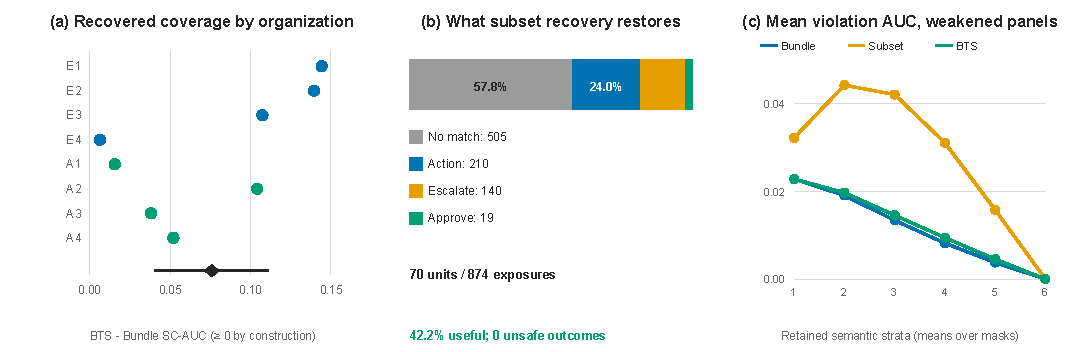
\includegraphics[width=\linewidth]{../figures/robustness_v04.pdf}
  \caption{Post-hoc diagnostics of the frozen v0.3 run. (a) BTS-minus-Bundle organization effects (E: expense; A: access), non-negative by construction, so they measure recovered coverage; the diamond is the cluster mean and bootstrap interval. (b) Aggregate outcomes in \RescueUnits{} subset-recovery units. (c) Mean violation AUC over exhaustive masks at each number of retained semantic verifier strata; per mask, BTS is lower/equal/higher in \CRMaskSemanticViolLower/\CRMaskSemanticViolEqual/\CRMaskSemanticViolHigher{} of these \CRMaskSemanticMasks{} masks (Appendix~\ref{app:masks}).}
  \label{fig:robustness}
\end{figure}

\paragraph{Recovery anatomy.}
Across \RescueUnits{} subset-recovery units (\RescueExposures{} hidden-task exposures), BTS produces \RescueActions{} successful actions, \RescueEscalations{} correct escalations, \RescueApprovals{} correct approvals, and \RescueNoMatches{} no-rule-match outcomes, so \RescueUsefulRate{} regain correct action or human routing, with no incorrect or unsafe outcome. All but two rescues occur at the first nonzero checkpoint: the gain is early acquisition, not terminal capability.

\paragraph{The verifier sets the safety ceiling.}
The full eight-case verifier exactly separates all \VerifierCandidates{} observed nonempty bundles: \VerifierTrueAccepts{} accepts are hidden-deployable and \VerifierTrueRejects{} rejects are not, with no false acceptances or rejections; the Gemini arm's \CRSepGemConfCandidates{} bundles separate just as exactly (\CRSepGemConfTrueAccepts{} and \CRSepGemConfTrueRejects{}). This is a synthetic-benchmark diagnostic, not evidence that eight tests suffice: verifier and hidden scenarios share a typed organization specification, and both labels are coarse binaries. We therefore exhaustively replay all \VerifierMasks{} nonempty verifier subsets, post-hoc, with stored candidates and zero model calls. Per mask, BTS's mean SC-AUC is never below Safe-Subset's (\CRMaskAllScLower/\CRMaskAllScEqual/\CRMaskAllScHigher{} masks lower/equal/higher, although \CRMaskSeriesScLower{} of \CRMaskSeriesTotal{} individual seed series are lower), but its violation exposure is lower in \CRMaskAllViolLower{} masks, equal in \CRMaskAllViolEqual{}, and higher in \CRMaskAllViolHigher{}, nearly even over the \CRMaskSemanticMasks{} semantic-strata masks of Figure~\ref{fig:robustness}(c) (\CRMaskSemanticViolLower/\CRMaskSemanticViolEqual/\CRMaskSemanticViolHigher), and the split turns on whether the panel keeps the escalation case D8 and the special-approval case D3 (Appendix~\ref{app:masks}). The coverage edge comes from the tie-break: Max-Subset (defined below) beats/ties/trails BTS's mean SC-AUC in \CRMaxMaskVsBtsScHigher/\CRMaxMaskVsBtsScEqual/\CRMaxMaskVsBtsScLower{} masks (trailing by at most \CRMaxMaskVsBtsMaxScDeficit{}), with lower/equal/higher violation exposure in \CRMaxMaskVsBtsViolLower/\CRMaxMaskVsBtsViolEqual/\CRMaxMaskVsBtsViolHigher. Omitting D3 alone creates \OmitApprovalFalseAccepts{} Bundle false acceptances (\OmitApprovalFalseAcceptRate{} of hidden-nondeployable bundles); BTS inherits them and reaches \OmitApprovalHybridViolation{} violation AUC, versus Safe-Subset's \OmitApprovalSubsetViolation{}. Omitting the escalation case alone leaves full-bundle separation intact but makes subset recovery unsafe (BTS \OmitEscalationHybridViolation{}; Safe-Subset \OmitEscalationSubsetViolation{}). BTS is not verifier-independent.

\paragraph{A designed blind spot isolates the mechanism.}
Because v0.3's verifier proved representative enough that its \PrunedPassingUnits{} accepted-bundle prunings left hidden coverage unchanged, a prospective stress arm (v0.5) designs the blind spot: six fresh organizations whose eight-case development panel contains no approval-outcome case, while their hidden panels are approval-rich; DSL, prompts, gates, metrics, and the v0.3 model configuration are unchanged ($6$ organizations $\times$ $5$ checkpoints $\times$ $3$ seeds $=90$ units; predictions and protocol frozen before the hidden matrix, after a two-organization development check; Appendix~\ref{app:freeze}). \textbf{P1} and \textbf{P2} are design-validation checks --- given the proposition, they are arithmetic consequences once candidates encode the blind obligation --- and both held: given the premise that every generated candidate encodes the approval obligation ($72/72$), exact subset search pruned the approval rules from every accepted bundle ($66/66$; P1), and Safe-Subset's hidden coverage fell below Bundle's and BTS's (P2). The empirical content lies in the premises holding for generated candidates at all, and in what follows. At the \emph{evidence-complete} checkpoints (16--32, where all $54/54$ accepted bundles pass the full development panel; a post-hoc stratum for v0.5, first named in the v0.5b protocol), the per-unit coverage loss equals the blind approval-task share \emph{exactly} in $54/54$ units, a six-organization mean of $\CRMaxDSApprBlindCompleteLoss$ that is a design constant ($\CRMaxDSApprBlindCompleteLossExpense$ expense, $\CRMaxDSApprBlindCompleteLossAccess$ access), so we report no interval. BTS equalled Bundle in every accepted unit and additionally recovered rejected units (overall SC-AUC $0.65$ versus $0.64$; Safe-Subset $0.36$; Figure~\ref{fig:stress}). \textbf{P3} (the pruning harm is lost coverage, not unsafe action) held too: approval-outcome tasks fall to no-rule-match abstention, and no violation is attributable to pruning.

The thin-evidence checkpoint adds an \emph{observed, unpredicted} boundary. From eight evidence items the blind panel accepted twelve weak bundles, ten of them falsely; those ten commit twenty hidden policy violations that Bundle and BTS inherit while Safe-Subset incidentally avoids them by pruning the offending rules, exactly the asymmetry anticipated in Section~2.

\paragraph{A second blind spot flips the failure shape.}
To test whether the mechanism is specific to the approval stratum, a second frozen arm (v0.5b) blinds the development panel to a different behavior: it contains both approval cases but no ineligible case, so the eligibility/escalation rule is the invisible one, and hidden panels carry every ineligible case (three per organization). Its organizations, evidence, prompts, and model configuration are byte-identical to v0.5, so the response cache gives both arms the \emph{same} candidates in $\CRPairDSCandidates$ of $\CRPairDSCandidatesTotal$ cases (one seed series was regenerated), a paired comparison (Appendix~\ref{app:freeze}). The pruning half repeats exactly: every candidate encoded the eligibility obligation ($72/72$), subset search pruned the escalation rule from every accepted bundle that carried it ($56/56$), and the per-unit coverage loss again equals the blind share exactly ($54/54$; mean $\CRMaxDSEscBlindCompleteLoss$). The exposure shape, however, flips, and our frozen point prediction fails: P3' predicted the benign shape at evidence-complete checkpoints, while committing to report whichever branch occurred. Twenty-six of the 54 evidence-complete accepted units relied on escalate-first rule order rather than an explicit eligibility guard in their tier rules; with the escalation rule pruned, those artifacts auto-execute ineligible requests, and Safe-Subset becomes the violating gate (52 hidden policy violations at the evidence-complete checkpoints) while Bundle and BTS commit none. The same exact coverage loss splits into benign abstention (28 units) and unsafe action (26 units) depending on a rule-order dependence that no coverage metric distinguishes; the safety-constrained metric does. Table~\ref{tab:stress} aligns the two arms.

Both designs were repeated with Gemini 3.7 Flash under jointly frozen successor protocols (Appendix~\ref{app:successors}). The mechanism transfers exactly: every candidate encodes the blind obligation, subset search prunes it from every accepted bundle, and coverage loss equals the blind share in $54/54$ evidence-complete units in both arms (Table~\ref{tab:stress}). The violation channel is candidate-dependent: Gemini relied on rule order in both arms ($16/54$ escalation-blind units, 32 violations; $5/54$ approval-blind units, 30 violations), so the benign-shape point prediction fails in both (for the escalation-blind arm the jointly frozen protocol text states only the disjunctive P3', which held, while the arm's freeze record also lists the benign point prediction; Appendix~\ref{app:successors}). What holds across models is the rule: pruning is benign exactly where the surviving rules guard the blind behavior, at evidence-complete checkpoints violations appear under Safe-Subset only, never under Bundle or BTS, and BTS preserved every accepted bundle in all four arms.

\paragraph{The failure is the tie-break.}
A post-hoc control isolates the damaging ingredient. \emph{Max-Subset} runs the identical exact search---same safety constraints, same pass maximization---except that ties break toward \emph{more} rules. Replaying every stored candidate through the frozen gates (zero model calls; both models, the confirmatory arms, and all four stress arms), Max-Subset retains the complete bundle in $\CRMaxAllKeepsBundle/\CRMaxAllAccepted$ accepted-bundle units and adds no violation of its own (its only violations are the inherited false acceptances below); its SC-AUC equals Safe-Subset's where nothing was ever lost (\CRMaxDSConfMaxSc{} and \CRMaxGemConfMaxSc{} in the two confirmatory arms) and exceeds BTS's on the escalation-blind rejected path, where its maximal rescued subsets carry more coverage than BTS's minimal ones (\CRMaxDSEscBlindMaxSc{} versus \CRMaxDSEscBlindBtsSc{} under DeepSeek; \CRMaxGemEscBlindMaxSc{} versus \CRMaxGemEscBlindBtsSc{} under Gemini); under approval blindness it ties or nearly ties (\CRMaxDSApprBlindMaxSc{} versus \CRMaxDSApprBlindBtsSc{}; \CRMaxGemApprBlindMaxSc{} versus \CRMaxGemApprBlindBtsSc{}). The over-pruning failure is therefore attributable to the parsimony tie-break, not to subset search: deleting verifier-invisible rules only ever ties, so the tie-break direction alone decides their fate. What conservative-first release adds over reversing the tie-break is not accuracy but less verifier work: BTS releases the same artifact on every accepted bundle without searching subsets, with \SubsetSearchReduction{} (DeepSeek) and \CREarlyGemConfSavingVsSubset{} (Gemini) fewer verifier artifact evaluations than plain enumeration, but at most \CREarlyDSConfSavingVsMaxEarly{} and \CREarlyGemConfSavingVsMaxEarly{} fewer than a Max-Subset search that stops once the complete bundle passes every case (Appendix~\ref{app:cost}). Its own recovery path still uses the fewer-rules tie-break; post-hoc variants that recover by descending from the bundle match or beat it under the full verifier with fewer evaluations (Appendix~\ref{app:cost}), so frozen BTS is not the best point in this design space. Like Bundle and BTS, Max-Subset inherits the thin-evidence false acceptances ($\CRMaxDSApprBlindViolations$ and $\CRMaxGemApprBlindViolations$ violations); reversing the tie-break is no protection against a verifier too weak to reject.

\begin{table}[t]
  \caption{\textbf{In all four arms, Safe-Subset prunes the blind rule from every accepted bundle; BTS never prunes any.} Two designed verifier blind spots, each over two models' candidates (six organizations; first two rows over all nonzero checkpoints, the rest evidence-complete unless noted; a model's two arms share \CRPairDSCandidates/\CRPairDSCandidatesTotal{} cached candidates under DeepSeek, \CRPairGemCandidates/\CRPairGemCandidatesTotal{} under Gemini). Coverage cost is the organization mean of per-unit accepted-bundle minus Safe-Subset hidden coverage; it agrees across models because the loss equals the designed blind share in every unit, a design constant reported without an interval, while violations depend on each model's rule order.}
  \label{tab:stress}
  \centering
  \small
  \setlength{\tabcolsep}{3.4pt}
  \begin{tabular}{lcccc}
    \toprule
    & \multicolumn{2}{c}{DeepSeek V4 Pro} & \multicolumn{2}{c}{Gemini 3.7 Flash} \\
    \cmidrule(lr){2-3}\cmidrule(lr){4-5}
    & Approval-blind & Escalation-blind & Approval-blind & Escalation-blind \\
    \midrule
    Candidates encoding blind obligation & $72/72$ & $72/72$ & $72/72$ & $72/72$ \\
    Accepted bundles, blind rule pruned & $66/66$ & $56/56$ & $66/66$ & $57/57$ \\
    Coverage loss $=$ blind share & $54/54$ & $54/54$ & $54/54$ & $54/54$ \\
    Coverage cost (= blind share, mean) & $\CRMaxDSApprBlindCompleteLoss$ & $\CRMaxDSEscBlindCompleteLoss$ & $\CRMaxGemApprBlindCompleteLoss$ & $\CRMaxGemEscBlindCompleteLoss$ \\
    Safe-Subset hidden violations & $0$ & $52$ (26 units) & $30$ (5 units) & $32$ (16 units) \\
    Bundle/BTS hidden violations & $20$ (thin-ev.) & $0$ & $18$ (thin-ev.) & $0$ \\
    BTS equals accepted Bundle & every unit & every unit & every unit & every unit \\
    \bottomrule
  \end{tabular}
\end{table}

\begin{figure}[t]
  \centering
  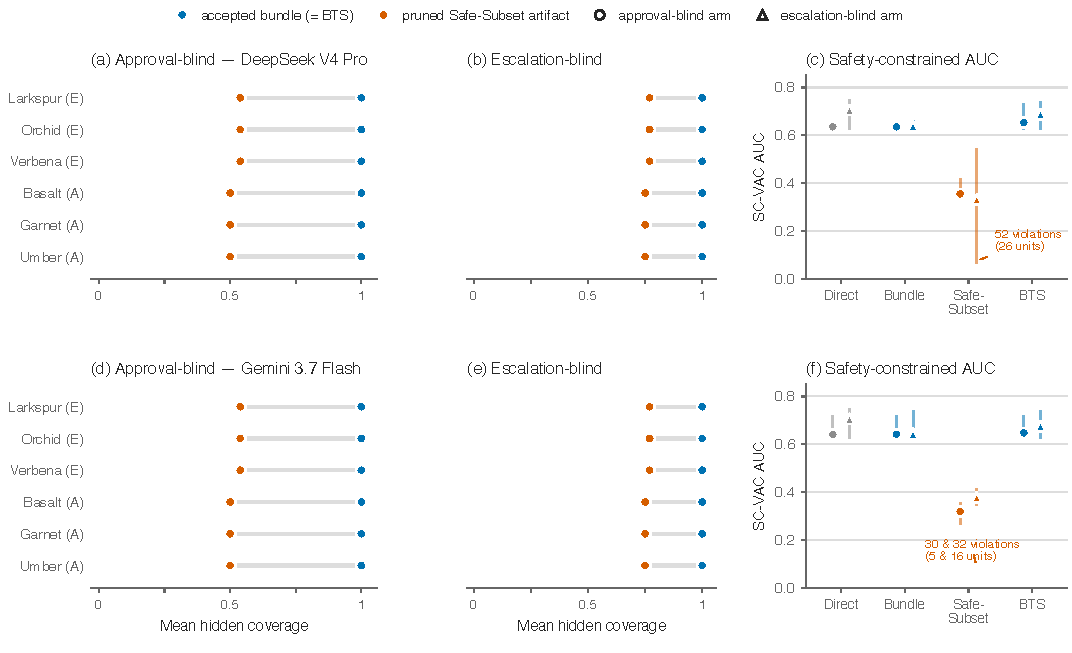
\includegraphics[width=\linewidth]{../figures/robustness_v05.pdf}
  \caption{The two designed-blind-spot stress arms (top: DeepSeek; bottom: Gemini; six shared organizations). (a, b, d, e) Mean hidden VAC per organization over the nine evidence-complete units: the accepted bundle, which BTS retains, versus the pruned Safe-Subset artifact; each gap equals that organization's blind-task share. (c, f) Safety-constrained AUC by gate; markers are cluster means (circles approval-blind, triangles escalation-blind), whiskers span organizations.}
  \label{fig:stress}
\end{figure}

A designed blind spot estimates no prevalence. The pair shows that when release tests cannot see a behavior, a fewer-rules search deletes it from every accepted candidate, and \emph{which} operator then looks safe depends on where the verifier is blind: in one arm conservative-first release inherits false acceptances that pruning would have removed; in the other, pruning manufactures the violations.

\paragraph{Retaining a bundle has a cost.}
On the \CRRetainDSConfAcceptedUnits{} v0.3 accepted units, Bundle and BTS release \CRRetainDSConfRulesBundle{} rules versus Safe-Subset's \CRRetainDSConfRulesSubset{} (\CRRetainDSConfExtraRulesPct{}) and make \CRRetainDSConfCondBundle{} versus \CRRetainDSConfCondSubset{} rule-condition evaluations per hidden task (\CRRetainDSConfCondPct{}). This v0.3 pruning is not verifier overfitting: acceptance needs only one pass and no policy or grounding failure, \CRPrunedDSConfAcceptedFailingCase{} of \CRPrunedDSConfAccepted{} accepted bundles fail some verifier case, and every non-dead pruned rule (\CRPrunedDSConfFireFail{} of \CRPrunedDSConfRules{}; Gemini \CRPrunedGemConfFireFail{} of \CRPrunedGemConfRules{}) fires on a verifier case and fails it. The \CRRetainDSConfExtraRules{} extra rules add no hidden success: \CRRetainDSConfDeadRules{} are dead, matching no verifier or hidden case, and the rest fire on \CRRetainDSConfFirings{} hidden task exposures with \CRRetainDSConfFiringPasses{} automated passes (\CRRetainDSConfOutcomeEscalationIncorrect{} incorrect escalations, \CRRetainDSConfOutcomeApprovalIncorrect{} incorrect approval requests, \CRRetainDSConfOutcomeActionFunctionalFailure{} functional failures, and \CRRetainDSConfOutcomeExplicitAbstention{} abstentions, all policy-safe), which Safe-Subset turns into no-rule-match, so VAC and SC-VAC are unchanged in all \CRRetainDSConfPrunedUnits{} pruned units. These are post-hoc, zero-model-call, DSL-level counts, not production latency; Appendix~\ref{app:cost} prices the stress arms.

\paragraph{Evidence timing does not replicate.}
The preregistered evidence-delay hypothesis (H3), the gap-3 minus gap-0 Direct raw-AUC effect, is \GapThreeDelta{} [\GapThreeCiLow{}, \GapThreeCiHigh{}], failing to replicate v0.2's $-0.090$ penalty; the Gemini arm instead shows $+0.095$ [$0.067$, $0.123$], so the model-stratified pooled $+0.042$ [$0.011$, $0.068$] is driven entirely by Gemini, and the point estimates differ in sign across arms. Post-hoc, the difference is confined to the \CRHThreeAccessOrgs{} access organizations (DeepSeek \CRHThreeAccessDS{}, Gemini \CRHThreeAccessGem{}; expense \CRHThreeExpenseDS{} versus \CRHThreeExpenseGem{}), and model is confounded with thinking level and serving stack, so we make neither a domain nor a model claim. Incomplete authorization did not consistently induce abstention and coincided with unsafe action in some access cases: presumed model conservatism is not a release control.

\section{Implications and related work}

The over-pruning is caused by the fewer-rules tie-break, not by subset search, so an accepted artifact should not be minimized with a size preference. Releasing it unchanged (BTS) or breaking ties toward more rules both avoid the failure, the latter equally well or better under the full verifier (Section~4); BTS's remaining edge is fewer verifier evaluations, and on the rejected path a descending or greedy recovery, tested under the full verifier only, matches or beats its frozen fewer-rules one with fewer evaluations (Appendix~\ref{app:cost}). Where verifier false acceptances are likely---thin evidence, or a panel lacking a decisive approval case---BTS inherits them while pruning may incidentally remove them; there the verifier, not the release operator, is the control to strengthen. The principle needs only a decomposable artifact and a verifier blind to some of its components, so it should transfer to tool-use plans, routing tables, or skill libraries with separable parts; where components interact, so that deleting one changes the verifier-visible behavior of others (as in free-text prompts), Proposition~1 does not apply.

Evidence timing yields no transferable monotonic rule: systems should explicitly detect incomplete threshold--authorization pairs rather than assume that the model will abstain. SC-VAC is deliberately artifact-level---one observed policy or grounding failure makes a checkpoint undeployable---so BTS's SC-AUC advantage over Direct is not raw-capability dominance; Table~\ref{tab:main} reports the raw loss and violation reduction side by side.

Our over-pruning result is candidate-relative regression within one rule-decomposable proposal, not the harness-level forgetting that HCL's finite retention anchors cannot rule out \citep{kang2026hcl}.

Finite-test selection is known to admit solutions that fail independently evaluated behavior in automated program repair \citep{smith2015overfitting}, where most patches reported by early generate-and-validate systems were incorrect and equivalent to deleting functionality \citep{qi2015kali}; our hidden scenarios serve this independent-evaluation role. Test-based debloating shows the same cost: removing never-executed code breaks needed functionality, which RAZOR counters with heuristics that retain related code \citep{qian2019razor} (BTS instead keeps the whole accepted artifact rather than inferring which unexercised parts matter), and dynamic-analysis-based debloaters remove up to 94\% of code that should be retained \citep{bilal2026debloating}. The designed blind spots are test-adequacy probes in the spirit of mutation testing, which seeds deliberate faults to measure what a test suite cannot see \citep{demillo1978mutation}. Safe policy improvement constrains deviation from a deployed baseline \citep{laroche2019spibb}, and Seldonian and high-confidence policy-improvement algorithms select a candidate on one data split, safety-test it on another, and otherwise return No Solution Found \citep{thomas2015hcpi,thomas2019seldonian}; BTS's accept/recover/abstain branches share that shape without a statistical guarantee. Cho and Sun give an always-valid rule for when an iterative generate--verify workflow should release, calibrating evaluator scores against hard-negative failures and accumulating evidence with an e-process \citep{cho2026release}; we instead ask what to release once a finite verifier has accepted a candidate.

Continual Harness edits prompts, sub-agents, skills, and memory online and studies model--harness co-learning \citep{karten2026continualharness}; we freeze the model and compare release operators. ExpeL and Agent Workflow Memory externalize reusable experience \citep{zhao2023expel,wang2025awm}; ADAS and harness-improvement work search agent programs or task harnesses \citep{hu2025adas,huang2026memoharness,zhou2026hsi}. WorkArena, $\tau$-bench, and CRMArena test agents in fixed enterprise environments \citep{drouin2024workarena,yao2024taubench,huang2025crmarena}. Our object is complementary: chronological organization acquisition under an external release controller.

\paragraph{Artifact availability.}
Hidden panels are disposable by design (each benchmark version was frozen with a fresh hidden split), so with all arms run the retired panels are released in full at \ArtifactURL{}: code and hidden-case constructors (Apache-2.0), and frozen specifications, freeze hashes, prompts, stored candidates, run records, and every post-hoc analysis (\mbox{CC-BY-4.0}). Its commands re-execute all 12,480 stored hidden gate evaluations with zero model calls and re-derive the outputs behind every reported number, requiring exact matches (Appendix~\ref{app:repro}). Credentials and raw provider responses are not released.

\section{Limitations and responsible use}

Organizations and tools are synthetic: eight parameterized organizations from two task-family templates in the confirmation and six in the stress arms, generated workflows of \CRRuleCountRangeWords{} rules (at most eight allowed), and verifier and hidden cases drawn from one typed specification per organization. That shared specification, together with coarse binary accept and deploy labels, likely explains why the full verifier separates every bundle in both confirmatory arms. All gates reach final VAC 1.000 under DeepSeek (0.990 under Gemini), and the evidence covers two temperature-zero models. The Gemini arm differs from the DeepSeek arm in thinking level and serving stack as well as in model, so the replication does not isolate the model factor, and two models do not establish generality across providers, scales, or sampling temperatures. The study therefore concerns acquisition trajectories under a small exact-search regime, not terminal capability or production-scale search cost. The cluster sample comprises these eight organizations; provider repetitions and bootstrap draws do not create additional organizations. The evidence intervention moves one policy and excludes noisy, adversarial, private, or continuously changing evidence. The v0.5 and v0.5b blind spots are designed, so they demonstrate a mechanism rather than estimating how often deployed verifiers are blind; undesigned rules that match no verifier case do occur in v0.3 (in \CRRetainDSConfUnmatchedRuleUnits{} of \CRRetainDSConfAcceptedUnits{} accepted DeepSeek bundles, none of Gemini's \CRRetainGemConfAcceptedUnits{}), but all are dead rules that match no hidden case either. The stress-split hidden panels are not comparable to v0.3's, and each model's two stress arms share cached candidates (a disclosed paired design, not independent samples). We leave to future work an adapted $\tau$-bench case (policy clause $\rightarrow$ conditional rule, API $\rightarrow$ declared tool, database-state check $\rightarrow$ verifier or hidden case); composition with a stateful updater that carries released artifacts forward; a release holdout separate from the verifier and hidden panels; coverage-preserving minimizers and recovery search where exhaustive enumeration is infeasible (BTS's accepted path needs none; Appendix~\ref{app:cost}); and non-rule artifacts such as prompts, routing policies, or tool-use plans.

Most importantly, BTS inherits accepted-bundle verifier errors by construction; its conservatism protects hidden-useful rules, not against false acceptance, just as resampling against an imperfect verifier cannot lower its false-positive probability \citep{stroebl2026limits}. v0.3 is the preregistered confirmation, replicated across both models, and the v0.5-family arms are prospective frozen stress tests; v0.2 BTS and every other analysis here, including all verifier-mask, Max-Subset, recovery-variant, cost, rescue, and organization- or domain-split results, are post-hoc diagnostics.

Production additionally requires access control, privacy review, human policy ownership, monitoring, rollback, and adversarial-evidence handling. We keep authorization, deterministic tests, and promotion outside the editable layer and make no production-readiness claim.

\clearpage
\bibliographystyle{plainnat}
\bibliography{references}

\appendix
\section{Freeze and audit}
\label{app:freeze}

Both phases retain immutable run sets and aggregate-only hidden artifacts. The v0.3 freeze pins the benchmark, the implementation and analysis code, and the prompt contract by cryptographic hash; the exact digests, together with every preserved v0.2 record, are part of the released archive rather than reproduced here.

The audit verified \ConfirmatoryUnits{} unique v0.3 units, all manifests/artifacts, all frozen v0.3 hashes, every preserved v0.2 hash, zero infrastructure failures, exhaustive mutually exclusive outcome counts, and no hidden task-level IDs, traces, grades, or failure strings.

The post-hoc v0.4 analysis preserves every frozen hash, makes zero model calls, reproduces all full-verifier gate-unit results, and then enumerates \VerifierMasks{} masks. The v0.5 stress arm carries its own frozen protocol, freeze record, zero-provider oracle validation, and audited 90-unit run set under the same contract. Its three predictions and full protocol were frozen before the hidden matrix ran, after a two-organization development check and after the zero-provider oracle validation had already established the mechanism at the oracle level; its evidence-complete stratum was named only later, in the v0.5b protocol. In v0.5 the evidence-complete coverage cost is $\CRMaxDSApprBlindCompleteLossExpense$ in the expense and $\CRMaxDSApprBlindCompleteLossAccess$ in the access organizations; the three access organizations coincide because their panels share size and approval share. Because v0.5b's organizations, evidence, prompts, and model configuration are byte-identical to v0.5, the deterministic response cache resolves v0.5b generations to the v0.5 responses, pairing $\CRPairDSCandidates$ of the $\CRPairDSCandidatesTotal$ candidates ($\CRPairDSUnits$ of $\CRPairDSUnitsTotal$ units). The exception is one seed series of one expense organization (four units) whose first v0.5 call terminated in each unit and was retried as the second permitted attempt; v0.5b regenerated them fresh in one attempt each, for all of its \$\CRPairDSUnpairedCost{} provider cost, so the frozen protocol's statement that the candidate hashes match holds for $\CRPairDSUnits$ of $\CRPairDSUnitsTotal$ units, and per-arm counts are computed on each arm's own candidates. The pairing is disclosed in the frozen protocol, and the v0.5b predictions were frozen before any v0.5b evaluation was computed. The v0.2 BTS reconstruction and all v0.4 analyses are labeled post-hoc and do not alter preregistered v0.3 H1--H3. Two preregistered mandatory outputs complete the v0.3 record: Direct's gap-1 minus gap-0 raw AUC is \GapOneDelta{} [\GapOneCiLow{}, \GapOneCiHigh{}], so the evidence-delay curve is not monotonic, and the weight $\lambda$ above which BTS's normalized functional AUC minus $\lambda$ times violation-exposure AUC exceeds Direct's lies between \LambdaLow{} and \LambdaHigh{} across the four gaps. Post-hoc, the model-by-gap interaction in H3 is \CRHThreeInteraction{} (t-interval [\CRHThreeInteractionCiLow{}, \CRHThreeInteractionCiHigh{}] over \CRHThreeInteractionOrgs{} organizations instantiating two templates; descriptive, not a test); the gap effect is negative under DeepSeek and positive under Gemini in \CRHThreeAccessSignFlipOrgs{} of \CRHThreeAccessOrgs{} access and \CRHThreeExpenseSignFlipOrgs{} of \CRHThreeExpenseOrgs{} expense organizations.

Relative to the reviewed version, this camera-ready adds post-hoc, zero-model-call analyses of stored candidates: the Max-Subset tie-break control and its per-mask replay, cross-model accept/reject concordance, full-verifier separation in the Gemini arm, per-mask verifier-ablation distributions (Appendix~\ref{app:masks}), verifier-work, early-exit, retained-rule, pruned-rule, and recovery-variant accounting (Appendix~\ref{app:cost}), and the v0.2 domain and H3 organization splits. None alters a preregistered result.

\section{Cross-model successor protocols}
\label{app:successors}

The Gemini arm executed under two successively frozen successor protocols, each recording a forced infrastructure deviation while inheriting every scientific element byte-identically. First, the provider rejects the frozen reasoning-off configuration for this model (an HTTP 400 response stating the minimal thinking level is unsupported for this model), so the arm runs at the lowest supported thinking level; reasoning level is part of the serving configuration, which is why the replication is reported as cross-model \emph{and} cross-configuration. A second configuration difference surfaced only after review: although the frozen model descriptor sets JSON mode for both arms, the Vertex adapter of the pinned client library does not forward that setting, so Gemini's structured output was enforced by the prompt and the schema-validating parser (which strips code fences) rather than by the provider. Second, the consumer Generative Language API stalled on provider-side capacity---sustained HTTP 503 responses degrading to timeout-length hangs, with 48 of 480 hidden units complete at the pre-stated decision point after a day of retries---so execution moved to the same model behind Vertex AI under a decision rule stated in advance; all 480 units then ran fresh on the new route, and the abandoned partial evidence is archived unpooled. Third, development on the new route surfaced candidates that pass schema validation but fail deterministic execution (for example, binding a non-numeric value to a numeric tool argument, which this model occasionally does and DeepSeek never did); a guard adopted before the freeze classifies such candidates as rejected generations; it fired on two of 32 eligible development units and zero of 384 eligible hidden units (the single rejected hidden generation exhausted its attempts without a valid structured output). Provider-capacity errors (HTTP 503/429) were classified as infrastructure failures and absorbed by the frozen retry rules; no scientific outcome was derived from a failed attempt. The arm's audit verified all 480 units, manifests, frozen hashes, and outcome counts with no hidden task-level retention. Billable cost was \$2.10 summed over every archived v0.3c run record, including an aborted first development launch and infrastructure retries. The successor freeze records, the transport-route protocol, and the guard's audit trail are part of the released archive.

The Gemini stress arms (v0.5g, v0.5bg) ran under jointly frozen successor protocols with the same benchmarks, panels, gates, and analysis, the Vertex transport route and execution-validity guard of the cross-model arm, and candidates fully cache-paired within the model ($90/90$ units). Every Gemini candidate encodes the blind obligation ($72/72$ in both arms), subset search prunes the blind rule from every accepted bundle ($66/66$ approval-blind, $57/57$ escalation-blind), and the coverage loss reproduces the DeepSeek cluster means to all reported digits ($\CRMaxGemApprBlindCompleteLoss$ and $\CRMaxGemEscBlindCompleteLoss$). In the escalation-blind arm $16$ of $54$ evidence-complete units relied on escalate-first ordering ($32$ Safe-Subset violations, against DeepSeek's $52$ across $26$ units); the arm's freeze record carries v0.5b's full P3', including the benign-shape point prediction at evidence-complete checkpoints (the jointly frozen successor protocol prose states only the disjunction, benign abstention or rule-order violations); the point prediction failed ($16$ of $54$ units violating), as it failed under DeepSeek in $26$ of $54$ units, and the disjunction held. Unlike DeepSeek, whose approval-blind arm was fully benign, $5$ of $54$ approval-blind units relied on approval-rule ordering ($30$ Safe-Subset violations), so the transferred P3 point prediction of a benign shape fails for Gemini's approval-blind arm, and the observed shape is reported per the frozen commitment. Counting against the freeze records, the benign-shape point prediction failed in three of the four arms, all but DeepSeek's approval-blind arm. The clean arm-determined flip is therefore DeepSeek-specific.

\section{Reproduction, compute, and assets}
\label{app:repro}

The released archive (\ArtifactURL) licenses code---the simulator, workflow DSL, gates, grader, hidden-case constructors, and analysis and audit scripts---under Apache-2.0, and specifications, protocols, freeze records, run records, analyses, and documentation under CC-BY-4.0. The hidden panels are disposable by design: each benchmark version (v0.2, v0.3, v0.5) was frozen on newly authored organizations with a fresh hidden split, and the cross-model (v0.3c, v0.5g, v0.5bg) and escalation-blind (v0.5b) arms reused their parent's organizations by prespecified design. All arms have run, so the retired v0.2--v0.5 panels are released in full: the four distinct benchmark constructors, their full frozen specifications, which re-hash to the frozen benchmark hashes, and all 2,539 archived run units with their stored candidates. Any stored candidate can therefore be re-evaluated on its hidden panel with zero model calls. Because the v0.5 organizations reuse the v0.3 evidence template under new skins, a future confirmation needs a new template, not only new organizations. A dataset card documents construction, schemas, intended research use, and limitations, and a contamination canary string marks the release documentation and the data files written by the release builder; analysis outputs and hash-frozen files stay byte-identical and are covered by the release manifest instead. Seven lines of non-scientific session wording in five hash-frozen protocol and freeze records are replaced in the release copies; an erratum lists each edited line, each edited file's frozen and released SHA-256, and a SHA-256 of each removed line.

Every command below makes zero model calls; none needs the network once the pinned figure environment is installed (a one-time \texttt{pip install}). \texttt{node artifact\_tools/audit-and-reproduce.mjs} re-derives every reported aggregate summary (v0.2, v0.3, v0.3c, and the four stress arms) from the run records with exact equality, recomputes the paper's result macros, and hash-verifies every archived run record. \texttt{node scripts/release-camera-ready.mjs} reruns the six camera-ready analyses that need only stored run records (verifier work, full-verifier separation, cross-model concordance, stress-arm cache pairing, v0.2 pruning by domain, and H3 by organization), regenerates the camera-ready macros and tables and Figures~\ref{fig:robustness} and~\ref{fig:cr-mask-paired}, and checks every camera-ready analysis output against frozen SHA-256 hashes; with \texttt{-{}-with-hidden} it also reruns, on the released hidden panels, the seven camera-ready analyses that re-evaluate hidden cases---the verifier-mask replay, the retained-rule accounting, the Max-Subset control, the recovery variants, the early-exit evaluation counts, the Max-Subset mask replay, and the pruned-rule verifier behavior---before the hash check. \texttt{node artifact\_tools/rerun-hidden.mjs} validates every constructor (oracle workflows on every v0.3--v0.5 development and hidden case; panel and gate checks for v0.2); re-executes all 12,480 stored hidden gate evaluations of the seven hidden runs (v0.2, v0.3, v0.3c, and the four stress arms) on their hidden panels and requires each rebuilt record to equal the stored one; re-aggregates the four stress-arm hidden summaries from those records; and reruns the v0.4 verifier ablation and retention replay with their audits, requiring byte-identical outputs. \texttt{node artifact\_tools/verify-release.mjs} checks every file against the release manifest, recomputes or erratum-attests all 121 hashes pinned by the eight freeze records, and reruns the hidden-run audits, which reproduce the released audit records byte for byte. \texttt{node toy/run-toy.mjs} runs the public toy benchmark.

Not released are credentials and raw provider responses (the provider-response cache; candidates are released as parsed workflows), so the original paid candidate generation cannot be replayed offline; regenerating candidates needs provider keys. Task-level traces were never persisted in any split; replaying stored candidates regenerates them. The v0.2 run-state file was not archived, so the frozen v0.2 audit script cannot rerun; its pinned hashes and run set are checked instead. Exploratory pilots and connectivity probes outside the archived run sets required additional provider calls; they support no reported result and are not part of the release.

The provider does not disclose serving hardware. The 480-unit v0.3 run had an observed asynchronous timestamp span of 23.4 minutes and cost \$\BillableCost{}. The 90-unit v0.5 stress arm used the same DeepSeek configuration and cost \$0.128 including its development stage, with zero infrastructure failures as classified by its frozen audit (the four first calls that terminated and were retried count as generation attempts; Appendix~\ref{app:freeze}); the paired v0.5b arm cost \$0.006, all for regenerating the one seed series that the cache did not pair (Appendix~\ref{app:freeze}). The 480-unit Gemini arm cost \$2.10 summed over every archived v0.3c run record (development, hidden, an aborted first development launch, and infrastructure retries), and the Gemini stress arms cost \$0.48 (approval-blind, including development on both transport routes) and \$0.00 (escalation-blind, fully cache-paired); provider-capacity errors (HTTP 503/429) were classified as infrastructure failures and absorbed by the frozen retry rules, and no scientific outcome was derived from a failed attempt. Deterministic validation and analysis used an 11-core Apple M3 Pro CPU with 18\,GB RAM, no GPU, and under 0.2\,GB local artifact storage; a v0.4 precomputed-output integrity audit completes in well under a second on that machine. The Max-Subset tie-break control is a zero-model-call replay of stored candidates through the frozen gates; its script and output are packaged in the archive. An earlier copy of that output summed the four evidence regimes of the confirmatory arms (a series-key bug); the values reported here were unaffected, and the released output is corrected.

The implementation uses Pi Agent Core and Pi AI v0.84.2 under the MIT License and TypeScript v7.0.2 under Apache-2.0. DeepSeek V4 Pro was accessed under the provider's API terms on August 22 (v0.3) and August 26 (v0.5), 2026; Gemini 3.7 Flash was accessed under Google's API terms via the Generative Language API and Vertex AI on August 26, 2026. The organizations and task instances are synthetic assets authored for this study; the released archive documents their construction, schemas, intended research use, and limitations, with the licenses above and third-party notices.

\section{Per-mask verifier ablation}
\label{app:masks}

This analysis is post-hoc, makes zero model calls, and covers the v0.3 DeepSeek arm only. The replay re-evaluates every stored candidate under each of the \CRMaskTotal{} nonempty subsets of the eight-case verifier (\CRMaskWeakened{} weakened panels plus the full panel) and reproduces the committed aggregate ablation; each mask is scored by its mean AUC over \CRMaskSeriesPerMask{} seed series. Table~\ref{tab:cr-masks} counts masks by the sign of the BTS-minus-Safe-Subset difference, and Figure~\ref{fig:cr-mask-paired} pairs each mask's coverage and violation changes. Averages favor BTS: across the eight leave-one-case-out masks, BTS retains \LeaveOneHybridScAuc{} SC-AUC with \LeaveOneHybridViolationAuc{} violation AUC, versus Safe-Subset's \LeaveOneSubsetScAuc{} and \LeaveOneSubsetViolationAuc{}; as one, two, then three of the six semantic strata are dropped ($\CRMaskDepthOneMasks$, $\CRMaskDepthTwoMasks$, and $\CRMaskDepthThreeMasks$ masks), Safe-Subset's mean SC-AUC falls $\CRMaskDepthOneSubsetSc \rightarrow \CRMaskDepthTwoSubsetSc \rightarrow \CRMaskDepthThreeSubsetSc$ while BTS's declines only $\CRMaskDepthOneBtsSc \rightarrow \CRMaskDepthTwoBtsSc \rightarrow \CRMaskDepthThreeBtsSc$ and Bundle $\CRMaskDepthOneBundleSc \rightarrow \CRMaskDepthTwoBundleSc \rightarrow \CRMaskDepthThreeBundleSc$, and Safe-Subset's mean violation exposure is $\CRMaskDepthOneRatio$, $\CRMaskDepthTwoRatio$, and $\CRMaskDepthThreeRatio$ times BTS's. Four facts qualify these averages. First, BTS's coverage is never below Safe-Subset's per mask or per organization, but can be below it at finer levels: its mean SC-AUC is below Safe-Subset's in no mask and in none of the \CRMaskOrgPairTotal{} organization--mask pairs, but it is lower in \CRMaskSeriesScLower{} of \CRMaskSeriesTotal{} seed series and \CRMaskCellScLower{} of \CRMaskCellTotal{} unit--mask cells. Second, the violation comparison is close to even over the semantic-strata masks of Figure~\ref{fig:robustness}(c) (\CRMaskSemanticViolLower/\CRMaskSemanticViolEqual/\CRMaskSemanticViolHigher{} lower/equal/higher) and depends mainly on the escalation case D8 and, when D8 is present, on the special-approval case D3: BTS is lower/equal/higher in \CRMaskDEightAbsentViolLower/\CRMaskDEightAbsentViolEqual/\CRMaskDEightAbsentViolHigher{} of the \CRMaskDEightAbsentMasks{} masks without D8 and in \CRMaskDEightPresentViolLower/\CRMaskDEightPresentViolEqual/\CRMaskDEightPresentViolHigher{} of the \CRMaskDEightPresentMasks{} with it. Of the \CRMaskHigherTotal{} masks where BTS is higher, \CRMaskHigherDEightNoDThree{} include D8 and omit D3 (all \CRMaskDEightNoDThreeMasks{} such masks), where Bundle falsely accepts and BTS inherits the error; \CRMaskHigherDEightDThree{} include both (of \CRMaskDEightDThreeMasks{} such masks), and \CRMaskHigherNoDEight{} omit D8. Third, against Bundle, BTS's violation exposure is never lower and is higher in \CRMaskBundleViolHigher{} of \CRMaskTotal{} masks (\CRMaskBundleViolLower/\CRMaskBundleViolEqual/\CRMaskBundleViolHigher), the price of recovering subsets with a weakened verifier. Fourth, BTS's coverage edge over Safe-Subset is a tie-break effect. Replayed on the same masks, Max-Subset's mean SC-AUC is higher/equal/lower than BTS's in \CRMaxMaskVsBtsScHigher/\CRMaxMaskVsBtsScEqual/\CRMaxMaskVsBtsScLower{} of \CRMaxMaskTotal{} masks (never lower by more than \CRMaxMaskVsBtsMaxScDeficit{}) and never below Safe-Subset's (\CRMaxMaskVsSubsetScHigher/\CRMaxMaskVsSubsetScEqual/\CRMaxMaskVsSubsetScLower); its violation exposure is lower/equal/higher than BTS's in \CRMaxMaskVsBtsViolLower/\CRMaxMaskVsBtsViolEqual/\CRMaxMaskVsBtsViolHigher{} masks. Over the \CRMaxMaskWeakened{} weakened panels its mean SC-AUC is \CRMaxMaskWeakMaxSc{} (BTS \CRMaxMaskWeakBtsSc{}, Bundle \CRMaxMaskWeakBundleSc{}, Safe-Subset \CRMaxMaskWeakSubsetSc{}) and its mean violation AUC \CRMaxMaskWeakMaxViol{} (BTS \CRMaxMaskWeakBtsViol{}, Bundle \CRMaxMaskWeakBundleViol{}, Safe-Subset \CRMaxMaskWeakSubsetViol{}). BTS with a more-rules recovery releases exactly Max-Subset's artifact in every unit of all \CRMaxMaskMaxrecIdentical{} masks. The masks are exhaustive subsets of one synthetic panel, not a sample of real verifiers.

% Generated by scripts/emit-results-cr.mjs -- do not edit by hand. Requires % Generated by scripts/emit-results-cr.mjs -- do not edit by hand.
% Camera-ready POST-HOC analyses added in response to reviews (CLEA #74);
% every input is a zero-model-call replay or re-aggregation of stored runs.
% Arm codes: DSConf = v0.3 DeepSeek, GemConf = v0.3c Gemini, DSDisc = v0.2 DeepSeek,
% DSApprBlind/DSEscBlind = v0.5/v0.5b, GemApprBlind/GemEscBlind = v0.5g/v0.5bg.
% --- Per-mask verifier replay, v0.3 DeepSeek (research/robustness_v04_mask_distribution.json)
\newcommand{\CRMaskTotal}{255}
\newcommand{\CRMaskWeakened}{254}
\newcommand{\CRMaskSemanticTotal}{63}
\newcommand{\CRMaskSeriesPerMask}{96}
\newcommand{\CRMaskStrataOneMasks}{6}
\newcommand{\CRMaskStrataOneViolLower}{2}
\newcommand{\CRMaskStrataOneViolEqual}{2}
\newcommand{\CRMaskStrataOneViolHigher}{2}
\newcommand{\CRMaskStrataOneScLower}{0}
\newcommand{\CRMaskStrataOneScEqual}{0}
\newcommand{\CRMaskStrataOneScHigher}{6}
\newcommand{\CRMaskStrataOneDeltaViol}{$-$0.0094}
\newcommand{\CRMaskStrataOneDeltaSc}{+0.453}
\newcommand{\CRMaskStrataTwoMasks}{15}
\newcommand{\CRMaskStrataTwoViolLower}{7}
\newcommand{\CRMaskStrataTwoViolEqual}{2}
\newcommand{\CRMaskStrataTwoViolHigher}{6}
\newcommand{\CRMaskStrataTwoScLower}{0}
\newcommand{\CRMaskStrataTwoScEqual}{0}
\newcommand{\CRMaskStrataTwoScHigher}{15}
\newcommand{\CRMaskStrataTwoDeltaViol}{$-$0.0245}
\newcommand{\CRMaskStrataTwoDeltaSc}{+0.417}
\newcommand{\CRMaskStrataThreeMasks}{20}
\newcommand{\CRMaskStrataThreeViolLower}{9}
\newcommand{\CRMaskStrataThreeViolEqual}{3}
\newcommand{\CRMaskStrataThreeViolHigher}{8}
\newcommand{\CRMaskStrataThreeScLower}{0}
\newcommand{\CRMaskStrataThreeScEqual}{0}
\newcommand{\CRMaskStrataThreeScHigher}{20}
\newcommand{\CRMaskStrataThreeDeltaViol}{$-$0.0275}
\newcommand{\CRMaskStrataThreeDeltaSc}{+0.344}
\newcommand{\CRMaskStrataFourMasks}{15}
\newcommand{\CRMaskStrataFourViolLower}{5}
\newcommand{\CRMaskStrataFourViolEqual}{5}
\newcommand{\CRMaskStrataFourViolHigher}{5}
\newcommand{\CRMaskStrataFourScLower}{0}
\newcommand{\CRMaskStrataFourScEqual}{0}
\newcommand{\CRMaskStrataFourScHigher}{15}
\newcommand{\CRMaskStrataFourDeltaViol}{$-$0.0216}
\newcommand{\CRMaskStrataFourDeltaSc}{+0.240}
\newcommand{\CRMaskStrataFiveMasks}{6}
\newcommand{\CRMaskStrataFiveViolLower}{1}
\newcommand{\CRMaskStrataFiveViolEqual}{4}
\newcommand{\CRMaskStrataFiveViolHigher}{1}
\newcommand{\CRMaskStrataFiveScLower}{0}
\newcommand{\CRMaskStrataFiveScEqual}{2}
\newcommand{\CRMaskStrataFiveScHigher}{4}
\newcommand{\CRMaskStrataFiveDeltaViol}{$-$0.0112}
\newcommand{\CRMaskStrataFiveDeltaSc}{+0.118}
\newcommand{\CRMaskStrataSixMasks}{1}
\newcommand{\CRMaskStrataSixViolLower}{0}
\newcommand{\CRMaskStrataSixViolEqual}{1}
\newcommand{\CRMaskStrataSixViolHigher}{0}
\newcommand{\CRMaskStrataSixScLower}{0}
\newcommand{\CRMaskStrataSixScEqual}{1}
\newcommand{\CRMaskStrataSixScHigher}{0}
\newcommand{\CRMaskStrataSixDeltaViol}{0.0000}
\newcommand{\CRMaskStrataSixDeltaSc}{0.000}
\newcommand{\CRMaskSemanticMasks}{63}
\newcommand{\CRMaskSemanticViolLower}{24}
\newcommand{\CRMaskSemanticViolEqual}{17}
\newcommand{\CRMaskSemanticViolHigher}{22}
\newcommand{\CRMaskSemanticScLower}{0}
\newcommand{\CRMaskSemanticScEqual}{3}
\newcommand{\CRMaskSemanticScHigher}{60}
\newcommand{\CRMaskSemanticDeltaViol}{$-$0.0217}
\newcommand{\CRMaskSemanticDeltaSc}{+0.320}
\newcommand{\CRMaskAllMasks}{255}
\newcommand{\CRMaskAllViolLower}{112}
\newcommand{\CRMaskAllViolEqual}{67}
\newcommand{\CRMaskAllViolHigher}{76}
\newcommand{\CRMaskAllScLower}{0}
\newcommand{\CRMaskAllScEqual}{21}
\newcommand{\CRMaskAllScHigher}{234}
\newcommand{\CRMaskAllDeltaViol}{$-$0.0279}
\newcommand{\CRMaskAllDeltaSc}{+0.284}
\newcommand{\CRMaskWeakenedSetMasks}{254}
\newcommand{\CRMaskWeakenedSetViolLower}{112}
\newcommand{\CRMaskWeakenedSetViolEqual}{66}
\newcommand{\CRMaskWeakenedSetViolHigher}{76}
\newcommand{\CRMaskWeakenedSetScLower}{0}
\newcommand{\CRMaskWeakenedSetScEqual}{20}
\newcommand{\CRMaskWeakenedSetScHigher}{234}
\newcommand{\CRMaskWeakenedSetDeltaViol}{$-$0.0280}
\newcommand{\CRMaskWeakenedSetDeltaSc}{+0.285}
\newcommand{\CRMaskDEightAbsentMasks}{127}
\newcommand{\CRMaskDEightAbsentViolLower}{112}
\newcommand{\CRMaskDEightAbsentViolEqual}{11}
\newcommand{\CRMaskDEightAbsentViolHigher}{4}
\newcommand{\CRMaskDEightAbsentScLower}{0}
\newcommand{\CRMaskDEightAbsentScEqual}{0}
\newcommand{\CRMaskDEightAbsentScHigher}{127}
\newcommand{\CRMaskDEightAbsentDeltaViol}{$-$0.0599}
\newcommand{\CRMaskDEightAbsentDeltaSc}{+0.460}
\newcommand{\CRMaskDEightPresentMasks}{128}
\newcommand{\CRMaskDEightPresentViolLower}{0}
\newcommand{\CRMaskDEightPresentViolEqual}{56}
\newcommand{\CRMaskDEightPresentViolHigher}{72}
\newcommand{\CRMaskDEightPresentScLower}{0}
\newcommand{\CRMaskDEightPresentScEqual}{21}
\newcommand{\CRMaskDEightPresentScHigher}{107}
\newcommand{\CRMaskDEightPresentDeltaViol}{+0.0039}
\newcommand{\CRMaskDEightPresentDeltaSc}{+0.108}
\newcommand{\CRMaskDEightNoDThreeMasks}{64}
\newcommand{\CRMaskDEightNoDThreeViolLower}{0}
\newcommand{\CRMaskDEightNoDThreeViolEqual}{0}
\newcommand{\CRMaskDEightNoDThreeViolHigher}{64}
\newcommand{\CRMaskDEightNoDThreeScLower}{0}
\newcommand{\CRMaskDEightNoDThreeScEqual}{0}
\newcommand{\CRMaskDEightNoDThreeScHigher}{64}
\newcommand{\CRMaskDEightNoDThreeDeltaViol}{+0.0064}
\newcommand{\CRMaskDEightNoDThreeDeltaSc}{+0.114}
\newcommand{\CRMaskDEightDThreeMasks}{64}
\newcommand{\CRMaskDEightDThreeViolLower}{0}
\newcommand{\CRMaskDEightDThreeViolEqual}{56}
\newcommand{\CRMaskDEightDThreeViolHigher}{8}
\newcommand{\CRMaskDEightDThreeScLower}{0}
\newcommand{\CRMaskDEightDThreeScEqual}{21}
\newcommand{\CRMaskDEightDThreeScHigher}{43}
\newcommand{\CRMaskDEightDThreeDeltaViol}{+0.0013}
\newcommand{\CRMaskDEightDThreeDeltaSc}{+0.102}
\newcommand{\CRMaskSizeOneMasks}{8}
\newcommand{\CRMaskSizeOneViolLower}{3}
\newcommand{\CRMaskSizeOneViolEqual}{3}
\newcommand{\CRMaskSizeOneViolHigher}{2}
\newcommand{\CRMaskSizeOneDeltaSc}{+0.451}
\newcommand{\CRMaskSizeTwoMasks}{28}
\newcommand{\CRMaskSizeTwoViolLower}{15}
\newcommand{\CRMaskSizeTwoViolEqual}{4}
\newcommand{\CRMaskSizeTwoViolHigher}{9}
\newcommand{\CRMaskSizeTwoDeltaSc}{+0.421}
\newcommand{\CRMaskSizeThreeMasks}{56}
\newcommand{\CRMaskSizeThreeViolLower}{31}
\newcommand{\CRMaskSizeThreeViolEqual}{6}
\newcommand{\CRMaskSizeThreeViolHigher}{19}
\newcommand{\CRMaskSizeThreeDeltaSc}{+0.365}
\newcommand{\CRMaskSizeFourMasks}{70}
\newcommand{\CRMaskSizeFourViolLower}{34}
\newcommand{\CRMaskSizeFourViolEqual}{13}
\newcommand{\CRMaskSizeFourViolHigher}{23}
\newcommand{\CRMaskSizeFourDeltaSc}{+0.291}
\newcommand{\CRMaskSizeFiveMasks}{56}
\newcommand{\CRMaskSizeFiveViolLower}{21}
\newcommand{\CRMaskSizeFiveViolEqual}{19}
\newcommand{\CRMaskSizeFiveViolHigher}{16}
\newcommand{\CRMaskSizeFiveDeltaSc}{+0.211}
\newcommand{\CRMaskSizeSixMasks}{28}
\newcommand{\CRMaskSizeSixViolLower}{7}
\newcommand{\CRMaskSizeSixViolEqual}{15}
\newcommand{\CRMaskSizeSixViolHigher}{6}
\newcommand{\CRMaskSizeSixDeltaSc}{+0.134}
\newcommand{\CRMaskSizeSevenMasks}{8}
\newcommand{\CRMaskSizeSevenViolLower}{1}
\newcommand{\CRMaskSizeSevenViolEqual}{6}
\newcommand{\CRMaskSizeSevenViolHigher}{1}
\newcommand{\CRMaskSizeSevenDeltaSc}{+0.064}
\newcommand{\CRMaskSizeEightMasks}{1}
\newcommand{\CRMaskSizeEightViolLower}{0}
\newcommand{\CRMaskSizeEightViolEqual}{1}
\newcommand{\CRMaskSizeEightViolHigher}{0}
\newcommand{\CRMaskSizeEightDeltaSc}{0.000}
\newcommand{\CRMaskSeriesTotal}{24,480}
\newcommand{\CRMaskSeriesScLower}{140}
\newcommand{\CRMaskSeriesScEqual}{3,129}
\newcommand{\CRMaskSeriesScHigher}{21,211}
\newcommand{\CRMaskCellTotal}{122,400}
\newcommand{\CRMaskCellScLower}{1,366}
\newcommand{\CRMaskOrgPairTotal}{2,040}
\newcommand{\CRMaskOrgPairScLower}{0}
\newcommand{\CRMaskOrgPairScEqual}{252}
\newcommand{\CRMaskOrgPairScHigher}{1,788}
\newcommand{\CRMaskHigherTotal}{76}
\newcommand{\CRMaskHigherDEightNoDThree}{64}
\newcommand{\CRMaskHigherDEightDThree}{8}
\newcommand{\CRMaskHigherNoDEight}{4}
\newcommand{\CRMaskDepthOneMasks}{6}
\newcommand{\CRMaskDepthOneSubsetSc}{0.566}
\newcommand{\CRMaskDepthOneBtsSc}{0.685}
\newcommand{\CRMaskDepthOneBundleSc}{0.628}
\newcommand{\CRMaskDepthOneRatio}{3.46}
\newcommand{\CRMaskDepthTwoMasks}{15}
\newcommand{\CRMaskDepthTwoSubsetSc}{0.425}
\newcommand{\CRMaskDepthTwoBtsSc}{0.665}
\newcommand{\CRMaskDepthTwoBundleSc}{0.627}
\newcommand{\CRMaskDepthTwoRatio}{3.29}
\newcommand{\CRMaskDepthThreeMasks}{20}
\newcommand{\CRMaskDepthThreeSubsetSc}{0.301}
\newcommand{\CRMaskDepthThreeBtsSc}{0.646}
\newcommand{\CRMaskDepthThreeBundleSc}{0.625}
\newcommand{\CRMaskDepthThreeRatio}{2.89}
\newcommand{\CRMaskBundleViolLower}{0}
\newcommand{\CRMaskBundleViolEqual}{157}
\newcommand{\CRMaskBundleViolHigher}{98}
\newcommand{\CRMaskBundleScLower}{0}
\newcommand{\CRMaskBundleScEqual}{31}
\newcommand{\CRMaskBundleScHigher}{224}

% --- Verifier work by rule count (research/verifier_work_by_rulecount.json)
\newcommand{\CRRuleCountMin}{2}
\newcommand{\CRRuleCountMax}{6}
\newcommand{\CRRuleCountRangeWords}{two to six}
\newcommand{\CRWorkDSDiscCandidates}{382}
\newcommand{\CRWorkDSDiscAccepted}{336}
\newcommand{\CRWorkDSDiscAcceptedAllPass}{228}
\newcommand{\CRWorkDSDiscAcceptRate}{88.0\%}
\newcommand{\CRWorkDSDiscSubsetEvals}{7,386}
\newcommand{\CRWorkDSDiscBtsEvals}{680}
\newcommand{\CRWorkDSDiscReduction}{90.8\%}
\newcommand{\CRWorkDSDiscBtsNoRetest}{634}
\newcommand{\CRWorkDSDiscReductionNoRetest}{91.4\%}
\newcommand{\CRWorkDSDiscRuleMin}{2}
\newcommand{\CRWorkDSDiscRuleMax}{6}
\newcommand{\CRWorkDSDiscAcceptedRulesBundle}{1,448}
\newcommand{\CRWorkDSDiscAcceptedRulesSubset}{1,151}
\newcommand{\CRWorkDSConfCandidates}{381}
\newcommand{\CRWorkDSConfAccepted}{311}
\newcommand{\CRWorkDSConfAcceptedAllPass}{226}
\newcommand{\CRWorkDSConfAcceptRate}{81.6\%}
\newcommand{\CRWorkDSConfSubsetEvals}{9,315}
\newcommand{\CRWorkDSConfBtsEvals}{1,063}
\newcommand{\CRWorkDSConfReduction}{88.6\%}
\newcommand{\CRWorkDSConfBtsNoRetest}{993}
\newcommand{\CRWorkDSConfReductionNoRetest}{89.3\%}
\newcommand{\CRWorkDSConfRuleMin}{3}
\newcommand{\CRWorkDSConfRuleMax}{6}
\newcommand{\CRWorkDSConfNThreeCandidates}{68}
\newcommand{\CRWorkDSConfNThreeAcceptRate}{29.4\%}
\newcommand{\CRWorkDSConfNThreeSubsetEvals}{476}
\newcommand{\CRWorkDSConfNThreeBtsEvals}{404}
\newcommand{\CRWorkDSConfNThreeReduction}{15.1\%}
\newcommand{\CRWorkDSConfNFourCandidates}{112}
\newcommand{\CRWorkDSConfNFourAcceptRate}{81.3\%}
\newcommand{\CRWorkDSConfNFourSubsetEvals}{1,680}
\newcommand{\CRWorkDSConfNFourBtsEvals}{427}
\newcommand{\CRWorkDSConfNFourReduction}{74.6\%}
\newcommand{\CRWorkDSConfNFiveCandidates}{172}
\newcommand{\CRWorkDSConfNFiveAcceptRate}{99.4\%}
\newcommand{\CRWorkDSConfNFiveSubsetEvals}{5,332}
\newcommand{\CRWorkDSConfNFiveBtsEvals}{203}
\newcommand{\CRWorkDSConfNFiveReduction}{96.2\%}
\newcommand{\CRWorkDSConfNSixCandidates}{29}
\newcommand{\CRWorkDSConfNSixAcceptRate}{100.0\%}
\newcommand{\CRWorkDSConfNSixSubsetEvals}{1,827}
\newcommand{\CRWorkDSConfNSixBtsEvals}{29}
\newcommand{\CRWorkDSConfNSixReduction}{98.4\%}
\newcommand{\CRWorkDSConfCpEightSubsetEvals}{905}
\newcommand{\CRWorkDSConfCpEightBtsEvals}{747}
\newcommand{\CRWorkDSConfCpSixteenSubsetEvals}{2,386}
\newcommand{\CRWorkDSConfCpSixteenBtsEvals}{124}
\newcommand{\CRWorkDSConfCpTwentyFourSubsetEvals}{2,824}
\newcommand{\CRWorkDSConfCpTwentyFourBtsEvals}{96}
\newcommand{\CRWorkDSConfCpThirtyTwoSubsetEvals}{3,200}
\newcommand{\CRWorkDSConfCpThirtyTwoBtsEvals}{96}
\newcommand{\CRWorkDSConfAcceptedRulesBundle}{1,453}
\newcommand{\CRWorkDSConfAcceptedRulesSubset}{1,326}
\newcommand{\CRUnitDSConfUnits}{480}
\newcommand{\CRUnitDSConfAcceptedEqual}{311}
\newcommand{\CRUnitDSConfAcceptedNotEqual}{0}
\newcommand{\CRUnitDSConfRecoveryUnits}{70}
\newcommand{\CRUnitDSConfRecoveryHigher}{70}
\newcommand{\CRUnitDSConfNoReleaseUnits}{99}
\newcommand{\CRUnitDSConfBundleLower}{0}
\newcommand{\CRUnitDSConfSubsetEqual}{480}
\newcommand{\CRUnitDSConfSubsetLower}{0}
\newcommand{\CRWorkGemConfCandidates}{383}
\newcommand{\CRWorkGemConfAccepted}{300}
\newcommand{\CRWorkGemConfAcceptedAllPass}{251}
\newcommand{\CRWorkGemConfAcceptRate}{78.3\%}
\newcommand{\CRWorkGemConfSubsetEvals}{5,133}
\newcommand{\CRWorkGemConfBtsEvals}{952}
\newcommand{\CRWorkGemConfReduction}{81.5\%}
\newcommand{\CRWorkGemConfBtsNoRetest}{869}
\newcommand{\CRWorkGemConfReductionNoRetest}{83.1\%}
\newcommand{\CRWorkGemConfRuleMin}{2}
\newcommand{\CRWorkGemConfRuleMax}{5}
\newcommand{\CRWorkGemConfNTwoCandidates}{3}
\newcommand{\CRWorkGemConfNTwoAcceptRate}{0.0\%}
\newcommand{\CRWorkGemConfNTwoSubsetEvals}{9}
\newcommand{\CRWorkGemConfNTwoBtsEvals}{12}
\newcommand{\CRWorkGemConfNTwoReduction}{$-$33.3\%}
\newcommand{\CRWorkGemConfNThreeCandidates}{128}
\newcommand{\CRWorkGemConfNThreeAcceptRate}{37.5\%}
\newcommand{\CRWorkGemConfNThreeSubsetEvals}{896}
\newcommand{\CRWorkGemConfNThreeBtsEvals}{688}
\newcommand{\CRWorkGemConfNThreeReduction}{23.2\%}
\newcommand{\CRWorkGemConfNFourCandidates}{224}
\newcommand{\CRWorkGemConfNFourAcceptRate}{100.0\%}
\newcommand{\CRWorkGemConfNFourSubsetEvals}{3,360}
\newcommand{\CRWorkGemConfNFourBtsEvals}{224}
\newcommand{\CRWorkGemConfNFourReduction}{93.3\%}
\newcommand{\CRWorkGemConfNFiveCandidates}{28}
\newcommand{\CRWorkGemConfNFiveAcceptRate}{100.0\%}
\newcommand{\CRWorkGemConfNFiveSubsetEvals}{868}
\newcommand{\CRWorkGemConfNFiveBtsEvals}{28}
\newcommand{\CRWorkGemConfNFiveReduction}{96.8\%}
\newcommand{\CRWorkGemConfCpEightSubsetEvals}{660}
\newcommand{\CRWorkGemConfCpEightBtsEvals}{665}
\newcommand{\CRWorkGemConfCpSixteenSubsetEvals}{1,264}
\newcommand{\CRWorkGemConfCpSixteenBtsEvals}{96}
\newcommand{\CRWorkGemConfCpTwentyFourSubsetEvals}{1,592}
\newcommand{\CRWorkGemConfCpTwentyFourBtsEvals}{96}
\newcommand{\CRWorkGemConfCpThirtyTwoSubsetEvals}{1,617}
\newcommand{\CRWorkGemConfCpThirtyTwoBtsEvals}{95}
\newcommand{\CRWorkGemConfAcceptedRulesBundle}{1,180}
\newcommand{\CRWorkGemConfAcceptedRulesSubset}{1,167}
\newcommand{\CRUnitGemConfUnits}{480}
\newcommand{\CRUnitGemConfAcceptedEqual}{300}
\newcommand{\CRUnitGemConfAcceptedNotEqual}{0}
\newcommand{\CRUnitGemConfRecoveryUnits}{83}
\newcommand{\CRUnitGemConfRecoveryHigher}{83}
\newcommand{\CRUnitGemConfNoReleaseUnits}{97}
\newcommand{\CRUnitGemConfBundleLower}{0}
\newcommand{\CRUnitGemConfSubsetEqual}{480}
\newcommand{\CRUnitGemConfSubsetLower}{0}
\newcommand{\CRWorkDSApprBlindCandidates}{72}
\newcommand{\CRWorkDSApprBlindAccepted}{66}
\newcommand{\CRWorkDSApprBlindAcceptedAllPass}{54}
\newcommand{\CRWorkDSApprBlindAcceptRate}{91.7\%}
\newcommand{\CRWorkDSApprBlindSubsetEvals}{2,520}
\newcommand{\CRWorkDSApprBlindBtsEvals}{122}
\newcommand{\CRWorkDSApprBlindReduction}{95.2\%}
\newcommand{\CRWorkDSApprBlindBtsNoRetest}{116}
\newcommand{\CRWorkDSApprBlindReductionNoRetest}{95.4\%}
\newcommand{\CRWorkDSApprBlindRuleMin}{3}
\newcommand{\CRWorkDSApprBlindRuleMax}{6}
\newcommand{\CRWorkDSApprBlindAcceptedRulesBundle}{327}
\newcommand{\CRWorkDSApprBlindAcceptedRulesSubset}{174}
\newcommand{\CRUnitDSApprBlindUnits}{90}
\newcommand{\CRUnitDSApprBlindAcceptedEqual}{66}
\newcommand{\CRUnitDSApprBlindAcceptedNotEqual}{0}
\newcommand{\CRUnitDSApprBlindRecoveryUnits}{6}
\newcommand{\CRUnitDSApprBlindRecoveryHigher}{6}
\newcommand{\CRUnitDSApprBlindNoReleaseUnits}{18}
\newcommand{\CRUnitDSApprBlindBundleLower}{0}
\newcommand{\CRUnitDSApprBlindSubsetEqual}{24}
\newcommand{\CRUnitDSApprBlindSubsetLower}{10}
\newcommand{\CRWorkDSEscBlindCandidates}{72}
\newcommand{\CRWorkDSEscBlindAccepted}{56}
\newcommand{\CRWorkDSEscBlindAcceptedAllPass}{54}
\newcommand{\CRWorkDSEscBlindAcceptRate}{77.8\%}
\newcommand{\CRWorkDSEscBlindSubsetEvals}{2,552}
\newcommand{\CRWorkDSEscBlindBtsEvals}{200}
\newcommand{\CRWorkDSEscBlindReduction}{92.2\%}
\newcommand{\CRWorkDSEscBlindBtsNoRetest}{184}
\newcommand{\CRWorkDSEscBlindReductionNoRetest}{92.8\%}
\newcommand{\CRWorkDSEscBlindRuleMin}{3}
\newcommand{\CRWorkDSEscBlindRuleMax}{6}
\newcommand{\CRWorkDSEscBlindAcceptedRulesBundle}{297}
\newcommand{\CRWorkDSEscBlindAcceptedRulesSubset}{212}
\newcommand{\CRUnitDSEscBlindUnits}{90}
\newcommand{\CRUnitDSEscBlindAcceptedEqual}{56}
\newcommand{\CRUnitDSEscBlindAcceptedNotEqual}{0}
\newcommand{\CRUnitDSEscBlindRecoveryUnits}{13}
\newcommand{\CRUnitDSEscBlindRecoveryHigher}{13}
\newcommand{\CRUnitDSEscBlindNoReleaseUnits}{21}
\newcommand{\CRUnitDSEscBlindBundleLower}{0}
\newcommand{\CRUnitDSEscBlindSubsetEqual}{34}
\newcommand{\CRUnitDSEscBlindSubsetLower}{0}
\newcommand{\CRWorkGemApprBlindCandidates}{72}
\newcommand{\CRWorkGemApprBlindAccepted}{66}
\newcommand{\CRWorkGemApprBlindAcceptedAllPass}{54}
\newcommand{\CRWorkGemApprBlindAcceptRate}{91.7\%}
\newcommand{\CRWorkGemApprBlindSubsetEvals}{1,048}
\newcommand{\CRWorkGemApprBlindBtsEvals}{114}
\newcommand{\CRWorkGemApprBlindReduction}{89.1\%}
\newcommand{\CRWorkGemApprBlindBtsNoRetest}{108}
\newcommand{\CRWorkGemApprBlindReductionNoRetest}{89.7\%}
\newcommand{\CRWorkGemApprBlindRuleMin}{3}
\newcommand{\CRWorkGemApprBlindRuleMax}{5}
\newcommand{\CRWorkGemApprBlindAcceptedRulesBundle}{258}
\newcommand{\CRWorkGemApprBlindAcceptedRulesSubset}{147}
\newcommand{\CRUnitGemApprBlindUnits}{90}
\newcommand{\CRUnitGemApprBlindAcceptedEqual}{66}
\newcommand{\CRUnitGemApprBlindAcceptedNotEqual}{0}
\newcommand{\CRUnitGemApprBlindRecoveryUnits}{6}
\newcommand{\CRUnitGemApprBlindRecoveryHigher}{6}
\newcommand{\CRUnitGemApprBlindNoReleaseUnits}{18}
\newcommand{\CRUnitGemApprBlindBundleLower}{0}
\newcommand{\CRUnitGemApprBlindSubsetEqual}{24}
\newcommand{\CRUnitGemApprBlindSubsetLower}{9}
\newcommand{\CRWorkGemEscBlindCandidates}{72}
\newcommand{\CRWorkGemEscBlindAccepted}{57}
\newcommand{\CRWorkGemEscBlindAcceptedAllPass}{54}
\newcommand{\CRWorkGemEscBlindAcceptRate}{79.2\%}
\newcommand{\CRWorkGemEscBlindSubsetEvals}{1,048}
\newcommand{\CRWorkGemEscBlindBtsEvals}{177}
\newcommand{\CRWorkGemEscBlindReduction}{83.1\%}
\newcommand{\CRWorkGemEscBlindBtsNoRetest}{162}
\newcommand{\CRWorkGemEscBlindReductionNoRetest}{84.5\%}
\newcommand{\CRWorkGemEscBlindRuleMin}{3}
\newcommand{\CRWorkGemEscBlindRuleMax}{5}
\newcommand{\CRWorkGemEscBlindAcceptedRulesBundle}{231}
\newcommand{\CRWorkGemEscBlindAcceptedRulesSubset}{171}
\newcommand{\CRUnitGemEscBlindUnits}{90}
\newcommand{\CRUnitGemEscBlindAcceptedEqual}{57}
\newcommand{\CRUnitGemEscBlindAcceptedNotEqual}{0}
\newcommand{\CRUnitGemEscBlindRecoveryUnits}{9}
\newcommand{\CRUnitGemEscBlindRecoveryHigher}{9}
\newcommand{\CRUnitGemEscBlindNoReleaseUnits}{24}
\newcommand{\CRUnitGemEscBlindBundleLower}{0}
\newcommand{\CRUnitGemEscBlindSubsetEqual}{33}
\newcommand{\CRUnitGemEscBlindSubsetLower}{0}

% --- Retained-rule cost accounting (research/retention_cost_accounting.json)
\newcommand{\CRRetainDSConfAcceptedUnits}{311}
\newcommand{\CRRetainDSConfRulesBundle}{1,453}
\newcommand{\CRRetainDSConfRulesSubset}{1,326}
\newcommand{\CRRetainDSConfExtraRules}{127}
\newcommand{\CRRetainDSConfExtraRulesPct}{+9.6\%}
\newcommand{\CRRetainDSConfPrunedUnits}{112}
\newcommand{\CRRetainDSConfHiddenTasks}{3,889}
\newcommand{\CRRetainDSConfCondBundle}{2.612}
\newcommand{\CRRetainDSConfCondSubset}{2.536}
\newcommand{\CRRetainDSConfCondPct}{+3.0\%}
\newcommand{\CRRetainDSConfCondBundleTaskW}{2.608}
\newcommand{\CRRetainDSConfCondSubsetTaskW}{2.533}
\newcommand{\CRRetainDSConfCondPctTaskW}{+3.0\%}
\newcommand{\CRRetainDSConfToolsBundle}{1.312}
\newcommand{\CRRetainDSConfToolsSubset}{1.299}
\newcommand{\CRRetainDSConfMultiBundle}{12.0\%}
\newcommand{\CRRetainDSConfMultiSubset}{10.4\%}
\newcommand{\CRRetainDSConfPreempt}{0}
\newcommand{\CRRetainDSConfFirings}{242}
\newcommand{\CRRetainDSConfFiringPasses}{0}
\newcommand{\CRRetainDSConfFiringPolicyFail}{0}
\newcommand{\CRRetainDSConfFiringPolicySafeNonPass}{242}
\newcommand{\CRRetainDSConfPrunedVerifierMatching}{96}
\newcommand{\CRRetainDSConfPrunedVerifierUnmatched}{31}
\newcommand{\CRRetainDSConfScChangedUnits}{0}
\newcommand{\CRRetainDSConfVacChangedUnits}{0}
\newcommand{\CRRetainDSConfUnmatchedRules}{31}
\newcommand{\CRRetainDSConfUnmatchedRuleUnits}{31}
\newcommand{\CRRetainDSConfDeadRules}{31}
\newcommand{\CRRetainDSConfOutcomeNoRuleMatch}{$-$242}
\newcommand{\CRRetainDSConfOutcomeExplicitAbstention}{10}
\newcommand{\CRRetainDSConfOutcomeEscalationIncorrect}{114}
\newcommand{\CRRetainDSConfOutcomeApprovalIncorrect}{92}
\newcommand{\CRRetainDSConfOutcomeActionFunctionalFailure}{26}
\newcommand{\CRRetainGemConfAcceptedUnits}{300}
\newcommand{\CRRetainGemConfRulesBundle}{1,180}
\newcommand{\CRRetainGemConfRulesSubset}{1,167}
\newcommand{\CRRetainGemConfExtraRules}{13}
\newcommand{\CRRetainGemConfExtraRulesPct}{+1.1\%}
\newcommand{\CRRetainGemConfPrunedUnits}{13}
\newcommand{\CRRetainGemConfHiddenTasks}{3,757}
\newcommand{\CRRetainGemConfCondBundle}{2.627}
\newcommand{\CRRetainGemConfCondSubset}{2.607}
\newcommand{\CRRetainGemConfCondPct}{+0.8\%}
\newcommand{\CRRetainGemConfCondBundleTaskW}{2.626}
\newcommand{\CRRetainGemConfCondSubsetTaskW}{2.605}
\newcommand{\CRRetainGemConfCondPctTaskW}{+0.8\%}
\newcommand{\CRRetainGemConfToolsBundle}{1.333}
\newcommand{\CRRetainGemConfToolsSubset}{1.329}
\newcommand{\CRRetainGemConfMultiBundle}{9.6\%}
\newcommand{\CRRetainGemConfMultiSubset}{9.3\%}
\newcommand{\CRRetainGemConfPreempt}{0}
\newcommand{\CRRetainGemConfFirings}{59}
\newcommand{\CRRetainGemConfFiringPasses}{0}
\newcommand{\CRRetainGemConfFiringPolicyFail}{0}
\newcommand{\CRRetainGemConfFiringPolicySafeNonPass}{59}
\newcommand{\CRRetainGemConfPrunedVerifierMatching}{13}
\newcommand{\CRRetainGemConfPrunedVerifierUnmatched}{0}
\newcommand{\CRRetainGemConfScChangedUnits}{0}
\newcommand{\CRRetainGemConfVacChangedUnits}{0}
\newcommand{\CRRetainGemConfUnmatchedRules}{0}
\newcommand{\CRRetainGemConfUnmatchedRuleUnits}{0}
\newcommand{\CRRetainGemConfDeadRules}{0}
\newcommand{\CRRetainGemConfOutcomeNoRuleMatch}{$-$59}
\newcommand{\CRRetainGemConfOutcomeExplicitAbstention}{18}
\newcommand{\CRRetainGemConfOutcomeApprovalIncorrect}{26}
\newcommand{\CRRetainGemConfOutcomeActionFunctionalFailure}{15}
\newcommand{\CRRetainDSApprBlindAcceptedUnits}{66}
\newcommand{\CRRetainDSApprBlindRulesBundle}{327}
\newcommand{\CRRetainDSApprBlindRulesSubset}{174}
\newcommand{\CRRetainDSApprBlindExtraRules}{153}
\newcommand{\CRRetainDSApprBlindExtraRulesPct}{+87.9\%}
\newcommand{\CRRetainDSApprBlindPrunedUnits}{66}
\newcommand{\CRRetainDSApprBlindHiddenTasks}{822}
\newcommand{\CRRetainDSApprBlindCondBundle}{2.994}
\newcommand{\CRRetainDSApprBlindCondSubset}{2.308}
\newcommand{\CRRetainDSApprBlindCondPct}{+29.7\%}
\newcommand{\CRRetainDSApprBlindCondBundleTaskW}{2.996}
\newcommand{\CRRetainDSApprBlindCondSubsetTaskW}{2.313}
\newcommand{\CRRetainDSApprBlindCondPctTaskW}{+29.6\%}
\newcommand{\CRRetainDSApprBlindToolsBundle}{0.910}
\newcommand{\CRRetainDSApprBlindToolsSubset}{0.719}
\newcommand{\CRRetainDSApprBlindMultiBundle}{3.8\%}
\newcommand{\CRRetainDSApprBlindMultiSubset}{3.0\%}
\newcommand{\CRRetainDSApprBlindPreempt}{0}
\newcommand{\CRRetainDSApprBlindFirings}{451}
\newcommand{\CRRetainDSApprBlindFiringPasses}{372}
\newcommand{\CRRetainDSApprBlindFiringPolicyFail}{20}
\newcommand{\CRRetainDSApprBlindFiringPolicySafeNonPass}{59}
\newcommand{\CRRetainDSApprBlindPrunedVerifierMatching}{13}
\newcommand{\CRRetainDSApprBlindPrunedVerifierUnmatched}{140}
\newcommand{\CRRetainDSApprBlindScChangedUnits}{66}
\newcommand{\CRRetainDSApprBlindVacChangedUnits}{66}
\newcommand{\CRRetainDSApprBlindUnmatchedRules}{140}
\newcommand{\CRRetainDSApprBlindUnmatchedRuleUnits}{66}
\newcommand{\CRRetainDSApprBlindDeadRules}{26}
\newcommand{\CRRetainDSApprBlindOutcomeNoRuleMatch}{$-$451}
\newcommand{\CRRetainDSApprBlindOutcomeApprovalCorrect}{372}
\newcommand{\CRRetainDSApprBlindOutcomeActionPolicyFailure}{20}
\newcommand{\CRRetainDSApprBlindOutcomeActionFunctionalFailure}{59}
\newcommand{\CRRetainDSEscBlindAcceptedUnits}{56}
\newcommand{\CRRetainDSEscBlindRulesBundle}{297}
\newcommand{\CRRetainDSEscBlindRulesSubset}{212}
\newcommand{\CRRetainDSEscBlindExtraRules}{85}
\newcommand{\CRRetainDSEscBlindExtraRulesPct}{+40.1\%}
\newcommand{\CRRetainDSEscBlindPrunedUnits}{56}
\newcommand{\CRRetainDSEscBlindHiddenTasks}{701}
\newcommand{\CRRetainDSEscBlindCondBundle}{2.458}
\newcommand{\CRRetainDSEscBlindCondSubset}{2.143}
\newcommand{\CRRetainDSEscBlindCondPct}{+14.7\%}
\newcommand{\CRRetainDSEscBlindCondBundleTaskW}{2.459}
\newcommand{\CRRetainDSEscBlindCondSubsetTaskW}{2.146}
\newcommand{\CRRetainDSEscBlindCondPctTaskW}{+14.6\%}
\newcommand{\CRRetainDSEscBlindToolsBundle}{1.018}
\newcommand{\CRRetainDSEscBlindToolsSubset}{1.152}
\newcommand{\CRRetainDSEscBlindMultiBundle}{11.3\%}
\newcommand{\CRRetainDSEscBlindMultiSubset}{0.0\%}
\newcommand{\CRRetainDSEscBlindPreempt}{79}
\newcommand{\CRRetainDSEscBlindFirings}{176}
\newcommand{\CRRetainDSEscBlindFiringPasses}{168}
\newcommand{\CRRetainDSEscBlindFiringPolicyFail}{0}
\newcommand{\CRRetainDSEscBlindFiringPolicySafeNonPass}{8}
\newcommand{\CRRetainDSEscBlindPrunedVerifierMatching}{2}
\newcommand{\CRRetainDSEscBlindPrunedVerifierUnmatched}{83}
\newcommand{\CRRetainDSEscBlindScChangedUnits}{56}
\newcommand{\CRRetainDSEscBlindVacChangedUnits}{56}
\newcommand{\CRRetainDSEscBlindUnmatchedRules}{83}
\newcommand{\CRRetainDSEscBlindUnmatchedRuleUnits}{56}
\newcommand{\CRRetainDSEscBlindDeadRules}{27}
\newcommand{\CRRetainDSEscBlindOutcomeNoRuleMatch}{$-$97}
\newcommand{\CRRetainDSEscBlindOutcomeEscalationCorrect}{168}
\newcommand{\CRRetainDSEscBlindOutcomeApprovalIncorrect}{$-$27}
\newcommand{\CRRetainDSEscBlindOutcomeActionPolicyFailure}{$-$52}
\newcommand{\CRRetainDSEscBlindOutcomeActionFunctionalFailure}{8}
\newcommand{\CRRetainGemApprBlindAcceptedUnits}{66}
\newcommand{\CRRetainGemApprBlindRulesBundle}{258}
\newcommand{\CRRetainGemApprBlindRulesSubset}{147}
\newcommand{\CRRetainGemApprBlindExtraRules}{111}
\newcommand{\CRRetainGemApprBlindExtraRulesPct}{+75.5\%}
\newcommand{\CRRetainGemApprBlindPrunedUnits}{66}
\newcommand{\CRRetainGemApprBlindHiddenTasks}{822}
\newcommand{\CRRetainGemApprBlindCondBundle}{2.944}
\newcommand{\CRRetainGemApprBlindCondSubset}{2.031}
\newcommand{\CRRetainGemApprBlindCondPct}{+44.9\%}
\newcommand{\CRRetainGemApprBlindCondBundleTaskW}{2.946}
\newcommand{\CRRetainGemApprBlindCondSubsetTaskW}{2.035}
\newcommand{\CRRetainGemApprBlindCondPctTaskW}{+44.8\%}
\newcommand{\CRRetainGemApprBlindToolsBundle}{0.879}
\newcommand{\CRRetainGemApprBlindToolsSubset}{0.790}
\newcommand{\CRRetainGemApprBlindMultiBundle}{9.2\%}
\newcommand{\CRRetainGemApprBlindMultiSubset}{1.9\%}
\newcommand{\CRRetainGemApprBlindPreempt}{30}
\newcommand{\CRRetainGemApprBlindFirings}{447}
\newcommand{\CRRetainGemApprBlindFiringPasses}{372}
\newcommand{\CRRetainGemApprBlindFiringPolicyFail}{18}
\newcommand{\CRRetainGemApprBlindFiringPolicySafeNonPass}{57}
\newcommand{\CRRetainGemApprBlindPrunedVerifierMatching}{17}
\newcommand{\CRRetainGemApprBlindPrunedVerifierUnmatched}{94}
\newcommand{\CRRetainGemApprBlindScChangedUnits}{66}
\newcommand{\CRRetainGemApprBlindVacChangedUnits}{66}
\newcommand{\CRRetainGemApprBlindUnmatchedRules}{94}
\newcommand{\CRRetainGemApprBlindUnmatchedRuleUnits}{61}
\newcommand{\CRRetainGemApprBlindDeadRules}{0}
\newcommand{\CRRetainGemApprBlindOutcomeNoRuleMatch}{$-$417}
\newcommand{\CRRetainGemApprBlindOutcomeApprovalCorrect}{372}
\newcommand{\CRRetainGemApprBlindOutcomeActionPolicyFailure}{$-$12}
\newcommand{\CRRetainGemApprBlindOutcomeActionFunctionalFailure}{57}
\newcommand{\CRRetainGemEscBlindAcceptedUnits}{57}
\newcommand{\CRRetainGemEscBlindRulesBundle}{231}
\newcommand{\CRRetainGemEscBlindRulesSubset}{171}
\newcommand{\CRRetainGemEscBlindExtraRules}{60}
\newcommand{\CRRetainGemEscBlindExtraRulesPct}{+35.1\%}
\newcommand{\CRRetainGemEscBlindPrunedUnits}{57}
\newcommand{\CRRetainGemEscBlindHiddenTasks}{714}
\newcommand{\CRRetainGemEscBlindCondBundle}{2.693}
\newcommand{\CRRetainGemEscBlindCondSubset}{2.309}
\newcommand{\CRRetainGemEscBlindCondPct}{+16.6\%}
\newcommand{\CRRetainGemEscBlindCondBundleTaskW}{2.693}
\newcommand{\CRRetainGemEscBlindCondSubsetTaskW}{2.307}
\newcommand{\CRRetainGemEscBlindCondPctTaskW}{+16.8\%}
\newcommand{\CRRetainGemEscBlindToolsBundle}{1.016}
\newcommand{\CRRetainGemEscBlindToolsSubset}{1.074}
\newcommand{\CRRetainGemEscBlindMultiBundle}{15.3\%}
\newcommand{\CRRetainGemEscBlindMultiSubset}{6.6\%}
\newcommand{\CRRetainGemEscBlindPreempt}{62}
\newcommand{\CRRetainGemEscBlindFirings}{183}
\newcommand{\CRRetainGemEscBlindFiringPasses}{171}
\newcommand{\CRRetainGemEscBlindFiringPolicyFail}{0}
\newcommand{\CRRetainGemEscBlindFiringPolicySafeNonPass}{12}
\newcommand{\CRRetainGemEscBlindPrunedVerifierMatching}{3}
\newcommand{\CRRetainGemEscBlindPrunedVerifierUnmatched}{57}
\newcommand{\CRRetainGemEscBlindScChangedUnits}{57}
\newcommand{\CRRetainGemEscBlindVacChangedUnits}{57}
\newcommand{\CRRetainGemEscBlindUnmatchedRules}{57}
\newcommand{\CRRetainGemEscBlindUnmatchedRuleUnits}{57}
\newcommand{\CRRetainGemEscBlindDeadRules}{0}
\newcommand{\CRRetainGemEscBlindOutcomeNoRuleMatch}{$-$121}
\newcommand{\CRRetainGemEscBlindOutcomeEscalationCorrect}{171}
\newcommand{\CRRetainGemEscBlindOutcomeApprovalIncorrect}{$-$30}
\newcommand{\CRRetainGemEscBlindOutcomeActionPolicyFailure}{$-$32}
\newcommand{\CRRetainGemEscBlindOutcomeActionFunctionalFailure}{12}

% --- Full-verifier separation (research/full_verifier_separation.json)
\newcommand{\CRSepDSConfCandidates}{381}
\newcommand{\CRSepDSConfTrueAccepts}{311}
\newcommand{\CRSepDSConfTrueRejects}{70}
\newcommand{\CRSepDSConfFalseAccepts}{0}
\newcommand{\CRSepDSConfFalseRejects}{0}
\newcommand{\CRSepGemConfCandidates}{383}
\newcommand{\CRSepGemConfTrueAccepts}{300}
\newcommand{\CRSepGemConfTrueRejects}{83}
\newcommand{\CRSepGemConfFalseAccepts}{0}
\newcommand{\CRSepGemConfFalseRejects}{0}
\newcommand{\CRSepDSApprBlindCandidates}{72}
\newcommand{\CRSepDSApprBlindTrueAccepts}{56}
\newcommand{\CRSepDSApprBlindTrueRejects}{6}
\newcommand{\CRSepDSApprBlindFalseAccepts}{10}
\newcommand{\CRSepDSApprBlindFalseRejects}{0}
\newcommand{\CRSepDSEscBlindCandidates}{72}
\newcommand{\CRSepDSEscBlindTrueAccepts}{56}
\newcommand{\CRSepDSEscBlindTrueRejects}{6}
\newcommand{\CRSepDSEscBlindFalseAccepts}{0}
\newcommand{\CRSepDSEscBlindFalseRejects}{10}
\newcommand{\CRSepGemApprBlindCandidates}{72}
\newcommand{\CRSepGemApprBlindTrueAccepts}{57}
\newcommand{\CRSepGemApprBlindTrueRejects}{6}
\newcommand{\CRSepGemApprBlindFalseAccepts}{9}
\newcommand{\CRSepGemApprBlindFalseRejects}{0}
\newcommand{\CRSepGemEscBlindCandidates}{72}
\newcommand{\CRSepGemEscBlindTrueAccepts}{57}
\newcommand{\CRSepGemEscBlindTrueRejects}{6}
\newcommand{\CRSepGemEscBlindFalseAccepts}{0}
\newcommand{\CRSepGemEscBlindFalseRejects}{9}

% --- Exploratory recovery variants, full verifier only (research/recovery_variants_posthoc.json)
\newcommand{\CRRecovDSConfExhaustiveEvals}{1,063}
\newcommand{\CRRecovDSConfExhaustiveSc}{0.704}
\newcommand{\CRRecovDSConfExhaustiveRecovered}{70}
\newcommand{\CRRecovDSConfExhaustiveMeanRules}{1.74}
\newcommand{\CRRecovDSConfExhaustivePolicyFailures}{0}
\newcommand{\CRRecovDSConfDescendEvals}{626}
\newcommand{\CRRecovDSConfDescendSc}{0.704}
\newcommand{\CRRecovDSConfDescendRecovered}{70}
\newcommand{\CRRecovDSConfDescendMeanRules}{2.30}
\newcommand{\CRRecovDSConfDescendPolicyFailures}{0}
\newcommand{\CRRecovDSConfGreedyEvals}{620}
\newcommand{\CRRecovDSConfGreedySc}{0.704}
\newcommand{\CRRecovDSConfGreedyRecovered}{70}
\newcommand{\CRRecovDSConfGreedyMeanRules}{2.30}
\newcommand{\CRRecovDSConfGreedyPolicyFailures}{0}
\newcommand{\CRRecovDSConfGreedyEvalShare}{58\%}
\newcommand{\CRRecovDSConfDescendEvalShare}{59\%}
\newcommand{\CRRecovGemConfExhaustiveEvals}{952}
\newcommand{\CRRecovGemConfExhaustiveSc}{0.705}
\newcommand{\CRRecovGemConfExhaustiveRecovered}{83}
\newcommand{\CRRecovGemConfExhaustiveMeanRules}{1.87}
\newcommand{\CRRecovGemConfExhaustivePolicyFailures}{0}
\newcommand{\CRRecovGemConfDescendEvals}{629}
\newcommand{\CRRecovGemConfDescendSc}{0.705}
\newcommand{\CRRecovGemConfDescendRecovered}{83}
\newcommand{\CRRecovGemConfDescendMeanRules}{1.96}
\newcommand{\CRRecovGemConfDescendPolicyFailures}{0}
\newcommand{\CRRecovGemConfGreedyEvals}{629}
\newcommand{\CRRecovGemConfGreedySc}{0.705}
\newcommand{\CRRecovGemConfGreedyRecovered}{83}
\newcommand{\CRRecovGemConfGreedyMeanRules}{1.96}
\newcommand{\CRRecovGemConfGreedyPolicyFailures}{0}
\newcommand{\CRRecovGemConfGreedyEvalShare}{66\%}
\newcommand{\CRRecovGemConfDescendEvalShare}{66\%}
\newcommand{\CRRecovDSApprBlindExhaustiveEvals}{122}
\newcommand{\CRRecovDSApprBlindExhaustiveSc}{0.653}
\newcommand{\CRRecovDSApprBlindExhaustiveRecovered}{6}
\newcommand{\CRRecovDSApprBlindExhaustiveMeanRules}{1.33}
\newcommand{\CRRecovDSApprBlindExhaustivePolicyFailures}{20}
\newcommand{\CRRecovDSApprBlindDescendEvals}{91}
\newcommand{\CRRecovDSApprBlindDescendSc}{0.657}
\newcommand{\CRRecovDSApprBlindDescendRecovered}{6}
\newcommand{\CRRecovDSApprBlindDescendMeanRules}{2.17}
\newcommand{\CRRecovDSApprBlindDescendPolicyFailures}{20}
\newcommand{\CRRecovDSApprBlindGreedyEvals}{91}
\newcommand{\CRRecovDSApprBlindGreedySc}{0.657}
\newcommand{\CRRecovDSApprBlindGreedyRecovered}{6}
\newcommand{\CRRecovDSApprBlindGreedyMeanRules}{2.17}
\newcommand{\CRRecovDSApprBlindGreedyPolicyFailures}{20}
\newcommand{\CRRecovDSApprBlindGreedyEvalShare}{75\%}
\newcommand{\CRRecovDSApprBlindDescendEvalShare}{75\%}
\newcommand{\CRRecovDSEscBlindExhaustiveEvals}{200}
\newcommand{\CRRecovDSEscBlindExhaustiveSc}{0.688}
\newcommand{\CRRecovDSEscBlindExhaustiveRecovered}{13}
\newcommand{\CRRecovDSEscBlindExhaustiveMeanRules}{1.00}
\newcommand{\CRRecovDSEscBlindExhaustivePolicyFailures}{0}
\newcommand{\CRRecovDSEscBlindDescendEvals}{131}
\newcommand{\CRRecovDSEscBlindDescendSc}{0.732}
\newcommand{\CRRecovDSEscBlindDescendRecovered}{13}
\newcommand{\CRRecovDSEscBlindDescendMeanRules}{2.15}
\newcommand{\CRRecovDSEscBlindDescendPolicyFailures}{0}
\newcommand{\CRRecovDSEscBlindGreedyEvals}{128}
\newcommand{\CRRecovDSEscBlindGreedySc}{0.732}
\newcommand{\CRRecovDSEscBlindGreedyRecovered}{13}
\newcommand{\CRRecovDSEscBlindGreedyMeanRules}{2.15}
\newcommand{\CRRecovDSEscBlindGreedyPolicyFailures}{0}
\newcommand{\CRRecovDSEscBlindGreedyEvalShare}{64\%}
\newcommand{\CRRecovDSEscBlindDescendEvalShare}{66\%}
\newcommand{\CRRecovGemApprBlindExhaustiveEvals}{114}
\newcommand{\CRRecovGemApprBlindExhaustiveSc}{0.647}
\newcommand{\CRRecovGemApprBlindExhaustiveRecovered}{6}
\newcommand{\CRRecovGemApprBlindExhaustiveMeanRules}{1.00}
\newcommand{\CRRecovGemApprBlindExhaustivePolicyFailures}{18}
\newcommand{\CRRecovGemApprBlindDescendEvals}{90}
\newcommand{\CRRecovGemApprBlindDescendSc}{0.647}
\newcommand{\CRRecovGemApprBlindDescendRecovered}{6}
\newcommand{\CRRecovGemApprBlindDescendMeanRules}{2.00}
\newcommand{\CRRecovGemApprBlindDescendPolicyFailures}{18}
\newcommand{\CRRecovGemApprBlindGreedyEvals}{90}
\newcommand{\CRRecovGemApprBlindGreedySc}{0.647}
\newcommand{\CRRecovGemApprBlindGreedyRecovered}{6}
\newcommand{\CRRecovGemApprBlindGreedyMeanRules}{2.00}
\newcommand{\CRRecovGemApprBlindGreedyPolicyFailures}{18}
\newcommand{\CRRecovGemApprBlindGreedyEvalShare}{79\%}
\newcommand{\CRRecovGemApprBlindDescendEvalShare}{79\%}
\newcommand{\CRRecovGemEscBlindExhaustiveEvals}{177}
\newcommand{\CRRecovGemEscBlindExhaustiveSc}{0.675}
\newcommand{\CRRecovGemEscBlindExhaustiveRecovered}{9}
\newcommand{\CRRecovGemEscBlindExhaustiveMeanRules}{1.00}
\newcommand{\CRRecovGemEscBlindExhaustivePolicyFailures}{0}
\newcommand{\CRRecovGemEscBlindDescendEvals}{135}
\newcommand{\CRRecovGemEscBlindDescendSc}{0.707}
\newcommand{\CRRecovGemEscBlindDescendRecovered}{9}
\newcommand{\CRRecovGemEscBlindDescendMeanRules}{2.00}
\newcommand{\CRRecovGemEscBlindDescendPolicyFailures}{0}
\newcommand{\CRRecovGemEscBlindGreedyEvals}{129}
\newcommand{\CRRecovGemEscBlindGreedySc}{0.707}
\newcommand{\CRRecovGemEscBlindGreedyRecovered}{9}
\newcommand{\CRRecovGemEscBlindGreedyMeanRules}{2.00}
\newcommand{\CRRecovGemEscBlindGreedyPolicyFailures}{0}
\newcommand{\CRRecovGemEscBlindGreedyEvalShare}{73\%}
\newcommand{\CRRecovGemEscBlindDescendEvalShare}{76\%}

% --- Max-Subset tie-break control (research/robustness_max_subset_baseline.json)
\newcommand{\CRMaxDSConfBundleSc}{0.628}
\newcommand{\CRMaxDSConfSubsetSc}{0.704}
\newcommand{\CRMaxDSConfBtsSc}{0.704}
\newcommand{\CRMaxDSConfMaxSc}{0.704}
\newcommand{\CRMaxDSConfEvals}{9,315}
\newcommand{\CRMaxDSConfViolations}{0}
\newcommand{\CRMaxGemConfBundleSc}{0.627}
\newcommand{\CRMaxGemConfSubsetSc}{0.705}
\newcommand{\CRMaxGemConfBtsSc}{0.705}
\newcommand{\CRMaxGemConfMaxSc}{0.705}
\newcommand{\CRMaxGemConfEvals}{5,133}
\newcommand{\CRMaxGemConfViolations}{0}
\newcommand{\CRMaxDSApprBlindBundleSc}{0.636}
\newcommand{\CRMaxDSApprBlindSubsetSc}{0.355}
\newcommand{\CRMaxDSApprBlindBtsSc}{0.653}
\newcommand{\CRMaxDSApprBlindMaxSc}{0.657}
\newcommand{\CRMaxDSApprBlindEvals}{2,520}
\newcommand{\CRMaxDSApprBlindViolations}{20}
\newcommand{\CRMaxDSApprBlindCompleteUnits}{54}
\newcommand{\CRMaxDSApprBlindCompleteLoss}{0.48}
\newcommand{\CRMaxDSApprBlindCompleteLossExpense}{0.46}
\newcommand{\CRMaxDSApprBlindCompleteLossAccess}{0.50}
\newcommand{\CRMaxDSEscBlindBundleSc}{0.638}
\newcommand{\CRMaxDSEscBlindSubsetSc}{0.332}
\newcommand{\CRMaxDSEscBlindBtsSc}{0.688}
\newcommand{\CRMaxDSEscBlindMaxSc}{0.732}
\newcommand{\CRMaxDSEscBlindEvals}{2,552}
\newcommand{\CRMaxDSEscBlindViolations}{0}
\newcommand{\CRMaxDSEscBlindCompleteUnits}{54}
\newcommand{\CRMaxDSEscBlindCompleteLoss}{0.24}
\newcommand{\CRMaxDSEscBlindCompleteLossExpense}{0.23}
\newcommand{\CRMaxDSEscBlindCompleteLossAccess}{0.25}
\newcommand{\CRMaxGemApprBlindBundleSc}{0.641}
\newcommand{\CRMaxGemApprBlindSubsetSc}{0.319}
\newcommand{\CRMaxGemApprBlindBtsSc}{0.647}
\newcommand{\CRMaxGemApprBlindMaxSc}{0.647}
\newcommand{\CRMaxGemApprBlindEvals}{1,048}
\newcommand{\CRMaxGemApprBlindViolations}{18}
\newcommand{\CRMaxGemApprBlindCompleteUnits}{54}
\newcommand{\CRMaxGemApprBlindCompleteLoss}{0.48}
\newcommand{\CRMaxGemApprBlindCompleteLossExpense}{0.46}
\newcommand{\CRMaxGemApprBlindCompleteLossAccess}{0.50}
\newcommand{\CRMaxGemEscBlindBundleSc}{0.644}
\newcommand{\CRMaxGemEscBlindSubsetSc}{0.379}
\newcommand{\CRMaxGemEscBlindBtsSc}{0.675}
\newcommand{\CRMaxGemEscBlindMaxSc}{0.707}
\newcommand{\CRMaxGemEscBlindEvals}{1,048}
\newcommand{\CRMaxGemEscBlindViolations}{0}
\newcommand{\CRMaxGemEscBlindCompleteUnits}{54}
\newcommand{\CRMaxGemEscBlindCompleteLoss}{0.24}
\newcommand{\CRMaxGemEscBlindCompleteLossExpense}{0.23}
\newcommand{\CRMaxGemEscBlindCompleteLossAccess}{0.25}
\newcommand{\CRMaxAllAccepted}{856}
\newcommand{\CRMaxAllKeepsBundle}{856}

% --- Cross-model accept/reject concordance, v0.3 vs v0.3c (research/robustness_cross_model_concordance.json)
\newcommand{\CRConcordUnits}{480}
\newcommand{\CRConcordMatched}{380}
\newcommand{\CRConcordMatchedAgree}{348}
\newcommand{\CRConcordThreeWay}{444}
\newcommand{\CRConcordCheckpointZero}{96}

% --- Stress-arm cache pairing (research/stress_arm_cache_pairing.json)
\newcommand{\CRPairDSCandidates}{68}
\newcommand{\CRPairDSCandidatesTotal}{72}
\newcommand{\CRPairDSUnits}{86}
\newcommand{\CRPairDSUnitsTotal}{90}
\newcommand{\CRPairDSUnpairedUnits}{4}
\newcommand{\CRPairDSUnpairedCost}{0.006}
\newcommand{\CRPairDSEscBlindCost}{0.006}
\newcommand{\CRPairGemCandidates}{72}
\newcommand{\CRPairGemCandidatesTotal}{72}
\newcommand{\CRPairGemUnits}{90}
\newcommand{\CRPairGemUnitsTotal}{90}
\newcommand{\CRPairGemUnpairedUnits}{0}
\newcommand{\CRPairGemUnpairedCost}{0.000}
\newcommand{\CRPairGemEscBlindCost}{0.000}

% --- Post-critique: verifier evaluations vs early-exit Max-Subset and recovery variants (research/early_exit_eval_counts.json)
\newcommand{\CREarlyDSConfCandidates}{381}
\newcommand{\CREarlyDSConfBundleAllPass}{226}
\newcommand{\CREarlyDSConfSubsetEvals}{9,315}
\newcommand{\CREarlyDSConfBtsEvals}{1,063}
\newcommand{\CREarlyDSConfMaxPlainEvals}{9,315}
\newcommand{\CREarlyDSConfMaxEarlyEvals}{2,159}
\newcommand{\CREarlyDSConfDescendEvals}{626}
\newcommand{\CREarlyDSConfGreedyEvals}{620}
\newcommand{\CREarlyDSConfSavingVsSubset}{88.6\%}
\newcommand{\CREarlyDSConfSavingVsMaxEarly}{50.8\%}
\newcommand{\CREarlyDSConfExtraVsDescend}{69.8\%}
\newcommand{\CREarlyDSConfExtraVsGreedy}{71.5\%}
\newcommand{\CREarlyGemConfCandidates}{383}
\newcommand{\CREarlyGemConfBundleAllPass}{251}
\newcommand{\CREarlyGemConfSubsetEvals}{5,133}
\newcommand{\CREarlyGemConfBtsEvals}{952}
\newcommand{\CREarlyGemConfMaxPlainEvals}{5,133}
\newcommand{\CREarlyGemConfMaxEarlyEvals}{1,171}
\newcommand{\CREarlyGemConfDescendEvals}{629}
\newcommand{\CREarlyGemConfGreedyEvals}{629}
\newcommand{\CREarlyGemConfSavingVsSubset}{81.5\%}
\newcommand{\CREarlyGemConfSavingVsMaxEarly}{18.7\%}
\newcommand{\CREarlyGemConfExtraVsDescend}{51.4\%}
\newcommand{\CREarlyGemConfExtraVsGreedy}{51.4\%}

% --- Post-critique: Max-Subset and BTS with Max-Subset recovery under the 255 verifier masks, v0.3 DeepSeek (research/max_subset_masks_posthoc.json)
\newcommand{\CRMaxMaskTotal}{255}
\newcommand{\CRMaxMaskWeakened}{254}
\newcommand{\CRMaxMaskVsBtsScHigher}{168}
\newcommand{\CRMaxMaskVsBtsScEqual}{66}
\newcommand{\CRMaxMaskVsBtsScLower}{21}
\newcommand{\CRMaxMaskVsBtsViolLower}{98}
\newcommand{\CRMaxMaskVsBtsViolEqual}{117}
\newcommand{\CRMaxMaskVsBtsViolHigher}{40}
\newcommand{\CRMaxMaskVsSubsetScHigher}{234}
\newcommand{\CRMaxMaskVsSubsetScEqual}{21}
\newcommand{\CRMaxMaskVsSubsetScLower}{0}
\newcommand{\CRMaxMaskVsSubsetViolLower}{112}
\newcommand{\CRMaxMaskVsSubsetViolEqual}{53}
\newcommand{\CRMaxMaskVsSubsetViolHigher}{90}
\newcommand{\CRMaxMaskVsBtsMaxScDeficit}{0.0009}
\newcommand{\CRMaxMaskWeakBundleSc}{0.623}
\newcommand{\CRMaxMaskWeakBundleViol}{0.0068}
\newcommand{\CRMaxMaskWeakSubsetSc}{0.375}
\newcommand{\CRMaxMaskWeakSubsetViol}{0.0363}
\newcommand{\CRMaxMaskWeakBtsSc}{0.660}
\newcommand{\CRMaxMaskWeakBtsViol}{0.0083}
\newcommand{\CRMaxMaskWeakMaxSc}{0.672}
\newcommand{\CRMaxMaskWeakMaxViol}{0.0071}
\newcommand{\CRMaxMaskMaxrecIdentical}{255}

% --- Post-critique: what Safe-Subset's pruned rules do on the verifier cases (research/pruned_rules_verifier_posthoc.json)
\newcommand{\CRPrunedDSConfAccepted}{311}
\newcommand{\CRPrunedDSConfAcceptedFailingCase}{85}
\newcommand{\CRPrunedDSConfUnits}{112}
\newcommand{\CRPrunedDSConfRules}{127}
\newcommand{\CRPrunedDSConfFireFail}{96}
\newcommand{\CRPrunedDSConfFireAllPass}{0}
\newcommand{\CRPrunedDSConfShadowed}{0}
\newcommand{\CRPrunedDSConfVerifierUnmatched}{31}
\newcommand{\CRPrunedDSConfDead}{31}
\newcommand{\CRPrunedDSConfFirings}{212}
\newcommand{\CRPrunedDSConfFiringsPassing}{0}
\newcommand{\CRPrunedGemConfAccepted}{300}
\newcommand{\CRPrunedGemConfAcceptedFailingCase}{49}
\newcommand{\CRPrunedGemConfUnits}{13}
\newcommand{\CRPrunedGemConfRules}{13}
\newcommand{\CRPrunedGemConfFireFail}{13}
\newcommand{\CRPrunedGemConfFireAllPass}{0}
\newcommand{\CRPrunedGemConfShadowed}{0}
\newcommand{\CRPrunedGemConfVerifierUnmatched}{0}
\newcommand{\CRPrunedGemConfDead}{0}
\newcommand{\CRPrunedGemConfFirings}{47}
\newcommand{\CRPrunedGemConfFiringsPassing}{0}

% --- Post-critique: v0.2 DeepSeek pruning events and harm by domain (research/v02_pruning_by_domain.json)
\newcommand{\CRVtwoPruneEvents}{219}
\newcommand{\CRVtwoPruneHarmful}{94}
\newcommand{\CRVtwoPruneHelpful}{0}
\newcommand{\CRVtwoPruneProcurementOrgs}{4}
\newcommand{\CRVtwoPruneProcurementEvents}{148}
\newcommand{\CRVtwoPruneProcurementHarmful}{94}
\newcommand{\CRVtwoPruneProcurementOrgsWithHarm}{4}
\newcommand{\CRVtwoPruneProcurementPerSeriesMin}{$-$0.073}
\newcommand{\CRVtwoPruneProcurementPerSeriesMax}{$-$0.056}
\newcommand{\CRVtwoPruneSupportOrgs}{4}
\newcommand{\CRVtwoPruneSupportEvents}{71}
\newcommand{\CRVtwoPruneSupportHarmful}{0}
\newcommand{\CRVtwoPruneSupportOrgsWithHarm}{0}
\newcommand{\CRVtwoPruneSupportPerSeriesMin}{0.000}
\newcommand{\CRVtwoPruneSupportPerSeriesMax}{0.000}

% --- Post-critique: per-organization H3 and model x evidence-gap interaction, not preregistered (research/h3_by_organization_posthoc.json)
\newcommand{\CRHThreeDSMean}{$-$0.011}
\newcommand{\CRHThreeGemMean}{+0.095}
\newcommand{\CRHThreeInteraction}{+0.107}
\newcommand{\CRHThreeInteractionCiLow}{+0.010}
\newcommand{\CRHThreeInteractionCiHigh}{+0.203}
\newcommand{\CRHThreeInteractionOrgsPositive}{5}
\newcommand{\CRHThreeInteractionOrgs}{8}
\newcommand{\CRHThreeAccessDS}{$-$0.085}
\newcommand{\CRHThreeAccessGem}{+0.122}
\newcommand{\CRHThreeAccessDiff}{+0.207}
\newcommand{\CRHThreeAccessSignFlipOrgs}{4}
\newcommand{\CRHThreeAccessOrgs}{4}
\newcommand{\CRHThreeExpenseDS}{+0.063}
\newcommand{\CRHThreeExpenseGem}{+0.069}
\newcommand{\CRHThreeExpenseDiff}{+0.006}
\newcommand{\CRHThreeExpenseSignFlipOrgs}{0}
\newcommand{\CRHThreeExpenseOrgs}{4}
.
\begin{table}[t]
  \caption{\textbf{Post-hoc, zero model calls; v0.3 DeepSeek only.} Per-mask comparison of BTS with Safe-Subset over the replayed verifier subsets. Each mask's metric is the mean AUC over its \CRMaskSeriesPerMask{} seed series; ``lower/equal/higher'' counts masks by the sign of BTS minus Safe-Subset violation-exposure AUC (ties within $10^{-12}$). The first block keeps whole semantic strata (Fig.~1(c) grouping); the full panel is the single six-strata mask and is included in both ``all'' rows. D3 is the special-approval case. Mean $\Delta$SC-AUC is never negative for any mask, but BTS has lower SC-AUC than Safe-Subset in \CRMaskSeriesScLower{} of \CRMaskSeriesTotal{} individual seed series. The violation sign depends mainly on the escalation case D8 and, when D8 is present, on D3: BTS is never lower with D8 and is higher in every D8 mask that omits D3; of the \CRMaskHigherTotal{} masks where BTS is higher, \CRMaskHigherDEightNoDThree{} include D8 and omit D3.}
  \label{tab:cr-masks}
  \centering
  \small
  \setlength{\tabcolsep}{3.6pt}
  \begin{tabular}{lrrrrrr}
    \toprule
    & & \multicolumn{3}{c}{BTS violation AUC} & & \\
    & & \multicolumn{3}{c}{vs.\ Safe-Subset} & & \\
    \cmidrule(lr){3-5}
    Mask group & Masks & Lower & Equal & Higher & Mean $\Delta$Viol. & Mean $\Delta$SC \\
    \midrule
    1 of 6 semantic strata & \CRMaskStrataOneMasks & \CRMaskStrataOneViolLower & \CRMaskStrataOneViolEqual & \CRMaskStrataOneViolHigher & \CRMaskStrataOneDeltaViol & \CRMaskStrataOneDeltaSc \\
    2 of 6 semantic strata & \CRMaskStrataTwoMasks & \CRMaskStrataTwoViolLower & \CRMaskStrataTwoViolEqual & \CRMaskStrataTwoViolHigher & \CRMaskStrataTwoDeltaViol & \CRMaskStrataTwoDeltaSc \\
    3 of 6 semantic strata & \CRMaskStrataThreeMasks & \CRMaskStrataThreeViolLower & \CRMaskStrataThreeViolEqual & \CRMaskStrataThreeViolHigher & \CRMaskStrataThreeDeltaViol & \CRMaskStrataThreeDeltaSc \\
    4 of 6 semantic strata & \CRMaskStrataFourMasks & \CRMaskStrataFourViolLower & \CRMaskStrataFourViolEqual & \CRMaskStrataFourViolHigher & \CRMaskStrataFourDeltaViol & \CRMaskStrataFourDeltaSc \\
    5 of 6 semantic strata & \CRMaskStrataFiveMasks & \CRMaskStrataFiveViolLower & \CRMaskStrataFiveViolEqual & \CRMaskStrataFiveViolHigher & \CRMaskStrataFiveDeltaViol & \CRMaskStrataFiveDeltaSc \\
    6 of 6 semantic strata & \CRMaskStrataSixMasks & \CRMaskStrataSixViolLower & \CRMaskStrataSixViolEqual & \CRMaskStrataSixViolHigher & \CRMaskStrataSixDeltaViol & \CRMaskStrataSixDeltaSc \\
    \midrule
    All semantic-strata masks & \CRMaskSemanticMasks & \CRMaskSemanticViolLower & \CRMaskSemanticViolEqual & \CRMaskSemanticViolHigher & \CRMaskSemanticDeltaViol & \CRMaskSemanticDeltaSc \\
    All case subsets & \CRMaskAllMasks & \CRMaskAllViolLower & \CRMaskAllViolEqual & \CRMaskAllViolHigher & \CRMaskAllDeltaViol & \CRMaskAllDeltaSc \\
    \midrule
    D8 (escalation) absent & \CRMaskDEightAbsentMasks & \CRMaskDEightAbsentViolLower & \CRMaskDEightAbsentViolEqual & \CRMaskDEightAbsentViolHigher & \CRMaskDEightAbsentDeltaViol & \CRMaskDEightAbsentDeltaSc \\
    D8 (escalation) present & \CRMaskDEightPresentMasks & \CRMaskDEightPresentViolLower & \CRMaskDEightPresentViolEqual & \CRMaskDEightPresentViolHigher & \CRMaskDEightPresentDeltaViol & \CRMaskDEightPresentDeltaSc \\
    \quad D8 present, D3 absent & \CRMaskDEightNoDThreeMasks & \CRMaskDEightNoDThreeViolLower & \CRMaskDEightNoDThreeViolEqual & \CRMaskDEightNoDThreeViolHigher & \CRMaskDEightNoDThreeDeltaViol & \CRMaskDEightNoDThreeDeltaSc \\
    \quad D8 present, D3 present & \CRMaskDEightDThreeMasks & \CRMaskDEightDThreeViolLower & \CRMaskDEightDThreeViolEqual & \CRMaskDEightDThreeViolHigher & \CRMaskDEightDThreeDeltaViol & \CRMaskDEightDThreeDeltaSc \\
    \bottomrule
  \end{tabular}
\end{table}


\begin{figure}[ht]
  \centering
  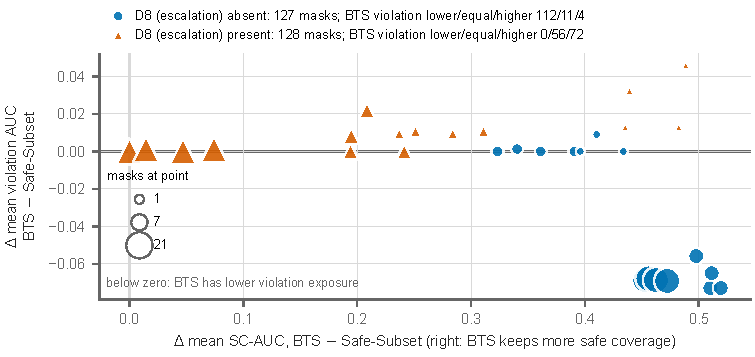
\includegraphics[width=0.92\linewidth]{../figures/mask_paired.pdf}
  \caption{\textbf{Post-hoc, zero model calls; v0.3 DeepSeek only.} Each point is a verifier mask: BTS minus Safe-Subset mean SC-AUC (horizontal) against mean violation AUC (vertical); marker area counts masks sharing a point. Color and shape mark whether the escalation case D8 is in the panel; without it BTS has lower violation exposure in most masks, with it never.}
  \label{fig:cr-mask-paired}
\end{figure}

\section{Verifier work, recovery variants, and the cost of retained rules}
\label{app:cost}

All analyses here are post-hoc and make zero model calls: verifier work is counted from stored run records, and retained-rule behavior from a replay of stored candidates through the frozen simulator and grader. Safe-Subset evaluates $2^n-1$ artifacts per $n$-rule candidate; BTS evaluates one if the bundle is accepted and $1+(2^n-1)$ otherwise. With full-bundle acceptance rate $a$ among $n$-rule candidates the reduction is therefore $a-1/(2^n-1)$, so it concentrates where acceptance is high (Table~\ref{tab:cr-verifier-work}): \CRWorkDSConfNThreeReduction{} for three-rule v0.3 candidates but \CRWorkDSConfNSixReduction{} for six-rule ones, \CRWorkDSConfReduction{} overall, and \CRWorkGemConfReduction{} in the Gemini arm (\CRWorkGemConfBtsEvals{} versus \CRWorkGemConfSubsetEvals{}). These savings assume that Safe-Subset is implemented, as here, by plain enumeration of all $2^n-1$ subsets. A pass-maximizing search that ties toward more rules could stop after testing the complete bundle whenever it passes every verifier case, as \CRWorkDSConfAcceptedAllPass{} of \CRWorkDSConfAccepted{} accepted DeepSeek and \CRWorkGemConfAcceptedAllPass{} of \CRWorkGemConfAccepted{} accepted Gemini bundles do; for the other accepted bundles the simple variant counted here enumerates every subset, whereas BTS stops at acceptance. Counted on the stored records, this early-exit Max-Subset needs \CREarlyDSConfMaxEarlyEvals{} (DeepSeek) and \CREarlyGemConfMaxEarlyEvals{} (Gemini) evaluations, so BTS's saving over it is \CREarlyDSConfSavingVsMaxEarly{} and \CREarlyGemConfSavingVsMaxEarly{} rather than \CREarlyDSConfSavingVsSubset{} and \CREarlyGemConfSavingVsSubset{}; a search that descends by subset size and stops at the first subset passing every case could need fewer, so these are upper bounds on BTS's saving over early-exit search. On the rejected path BTS pays whatever its recovery search costs, so for a rule-count group that is always rejected it pays more than Safe-Subset (Gemini's two-rule candidates: \CRWorkGemConfNTwoBtsEvals{} versus \CRWorkGemConfNTwoSubsetEvals{}).

Table~\ref{tab:cr-retention} prices retention in every arm. In the confirmatory arms the rules that Bundle and BTS keep but Safe-Subset prunes never produce an automated hidden pass, and none of them fires before a rule Safe-Subset kept on any of the \CRRetainDSConfHiddenTasks{} (DeepSeek) and \CRRetainGemConfHiddenTasks{} (Gemini) hidden tasks of accepted units; Gemini keeps only \CRRetainGemConfExtraRules{} extra rules and has no dead rules. In the stress arms the retained rules carry the blind behavior; they also fire before a rule Safe-Subset kept on \CRRetainDSEscBlindPreempt{} of \CRRetainDSEscBlindHiddenTasks{} (DeepSeek) and \CRRetainGemEscBlindPreempt{} of \CRRetainGemEscBlindHiddenTasks{} (Gemini) escalation-blind hidden tasks and on \CRRetainGemApprBlindPreempt{} of \CRRetainGemApprBlindHiddenTasks{} in Gemini's approval-blind arm. Whether a misrouted escalation costs more than an abstention is a deployment judgment. Latency, memory, and interference beyond first-match overlap are not measured.

Table~\ref{tab:cr-recovery} reports two cheaper recovery searches, designed post-hoc after the Max-Subset control and evaluated only with the full eight-case verifier, never under weakened masks; they are exploratory. Descent tries subsets from the largest size down and keeps the most-passing safe subset of the first size that has one (remaining ties go to the first in enumeration order); greedy drops one rule at a time. Both need fewer verifier evaluations than frozen BTS because they do not enumerate every subset (\CRRecovDSConfDescendEvalShare{} and \CRRecovGemConfDescendEvalShare{} of BTS's under descent in the confirmatory arms), and both match or exceed its SC-AUC in every arm because they rescue larger subsets (mean \CRRecovDSConfDescendMeanRules{} versus \CRRecovDSConfExhaustiveMeanRules{} rules in DeepSeek v0.3) and so avoid the fewer-rules tie-break on the rejected path. Frozen BTS is therefore not the best point in this design space, and the \CRWorkDSConfReduction{} saving over plain enumeration is not the best attainable figure either.

\paragraph{Larger search spaces.} Exhaustive enumeration grows as $2^n$, but BTS searches only on its rejected path: an accepted bundle costs one verifier evaluation whatever $n$ is, so with full-bundle acceptance rate $a$ the expected work per $n$-rule candidate is $1+(1-a)\,R(n)$, where $R(n)$ is the mean number of evaluations the recovery search spends on a rejected candidate ($2^n-1$ for exhaustive search, which re-tests the bundle). Where enumeration is infeasible, a cheaper search can fill that role: greedy deletion needs $O(n^2)$ evaluations, descending subset sizes $O(n^d)$ when $d$ rules must be dropped (exponential in the worst case), and delta debugging is another option. By the argument of Proposition~1, which does not use acceptance, any search run to 1-minimality (as delta debugging is) removes every rule that no verifier case matches, because deleting such a rule never changes a verifier outcome. Descend avoids this by construction, since it returns a largest passing subset; greedy stops at the first passing subset on its deletion path, which keeps such rules unless a tied deletion earlier on the path removed one. In v0.3 they matched exhaustive SC-AUC with \CRRecovDSConfDescendEvalShare{} (descend) and \CRRecovDSConfGreedyEvalShare{} (greedy) of its evaluations under DeepSeek and \CRRecovGemConfDescendEvalShare{} under Gemini (Table~\ref{tab:cr-recovery}). These variants are post-hoc and were evaluated only under the full verifier, and their searches ran only on rejected candidates of at most five rules, most of them three; behavior with larger artifacts, weakened verifier masks, or stochastic and expensive verifiers is untested.

\begin{table}[ht]
  \caption{\textbf{Post-hoc, zero model calls; designed after the Max-Subset control.} Recovery variants of BTS: each releases an accepted bundle unchanged and differs only in its search after rejection. Exhaustive (frozen BTS) enumerates all subsets with ties toward fewer rules; \emph{descend} tries subset sizes from $n-1$ downward and stops at the first size with a safe subset that passes a case; \emph{greedy} deletes one rule at a time. Cells give SC-AUC / total verifier artifact evaluations under the full verifier.}
  \label{tab:cr-recovery}
  \centering
  \footnotesize
  \setlength{\tabcolsep}{3pt}
  \begin{tabular}{lcccccc}
    \toprule
    & \multicolumn{2}{c}{v0.3 confirmation} & \multicolumn{2}{c}{Approval-blind} & \multicolumn{2}{c}{Escalation-blind} \\
    \cmidrule(lr){2-3}\cmidrule(lr){4-5}\cmidrule(lr){6-7}
    Recovery & DeepSeek & Gemini & DeepSeek & Gemini & DeepSeek & Gemini \\
    \midrule
    Exhaustive (BTS) & \CRRecovDSConfExhaustiveSc{} / \CRRecovDSConfExhaustiveEvals & \CRRecovGemConfExhaustiveSc{} / \CRRecovGemConfExhaustiveEvals & \CRRecovDSApprBlindExhaustiveSc{} / \CRRecovDSApprBlindExhaustiveEvals & \CRRecovGemApprBlindExhaustiveSc{} / \CRRecovGemApprBlindExhaustiveEvals & \CRRecovDSEscBlindExhaustiveSc{} / \CRRecovDSEscBlindExhaustiveEvals & \CRRecovGemEscBlindExhaustiveSc{} / \CRRecovGemEscBlindExhaustiveEvals \\
    Descend & \CRRecovDSConfDescendSc{} / \CRRecovDSConfDescendEvals & \CRRecovGemConfDescendSc{} / \CRRecovGemConfDescendEvals & \CRRecovDSApprBlindDescendSc{} / \CRRecovDSApprBlindDescendEvals & \CRRecovGemApprBlindDescendSc{} / \CRRecovGemApprBlindDescendEvals & \CRRecovDSEscBlindDescendSc{} / \CRRecovDSEscBlindDescendEvals & \CRRecovGemEscBlindDescendSc{} / \CRRecovGemEscBlindDescendEvals \\
    Greedy & \CRRecovDSConfGreedySc{} / \CRRecovDSConfGreedyEvals & \CRRecovGemConfGreedySc{} / \CRRecovGemConfGreedyEvals & \CRRecovDSApprBlindGreedySc{} / \CRRecovDSApprBlindGreedyEvals & \CRRecovGemApprBlindGreedySc{} / \CRRecovGemApprBlindGreedyEvals & \CRRecovDSEscBlindGreedySc{} / \CRRecovDSEscBlindGreedyEvals & \CRRecovGemEscBlindGreedySc{} / \CRRecovGemEscBlindGreedyEvals \\
    \bottomrule
  \end{tabular}
\end{table}

% Generated by scripts/emit-results-cr.mjs -- do not edit by hand. Requires % Generated by scripts/emit-results-cr.mjs -- do not edit by hand.
% Camera-ready POST-HOC analyses added in response to reviews (CLEA #74);
% every input is a zero-model-call replay or re-aggregation of stored runs.
% Arm codes: DSConf = v0.3 DeepSeek, GemConf = v0.3c Gemini, DSDisc = v0.2 DeepSeek,
% DSApprBlind/DSEscBlind = v0.5/v0.5b, GemApprBlind/GemEscBlind = v0.5g/v0.5bg.
% --- Per-mask verifier replay, v0.3 DeepSeek (research/robustness_v04_mask_distribution.json)
\newcommand{\CRMaskTotal}{255}
\newcommand{\CRMaskWeakened}{254}
\newcommand{\CRMaskSemanticTotal}{63}
\newcommand{\CRMaskSeriesPerMask}{96}
\newcommand{\CRMaskStrataOneMasks}{6}
\newcommand{\CRMaskStrataOneViolLower}{2}
\newcommand{\CRMaskStrataOneViolEqual}{2}
\newcommand{\CRMaskStrataOneViolHigher}{2}
\newcommand{\CRMaskStrataOneScLower}{0}
\newcommand{\CRMaskStrataOneScEqual}{0}
\newcommand{\CRMaskStrataOneScHigher}{6}
\newcommand{\CRMaskStrataOneDeltaViol}{$-$0.0094}
\newcommand{\CRMaskStrataOneDeltaSc}{+0.453}
\newcommand{\CRMaskStrataTwoMasks}{15}
\newcommand{\CRMaskStrataTwoViolLower}{7}
\newcommand{\CRMaskStrataTwoViolEqual}{2}
\newcommand{\CRMaskStrataTwoViolHigher}{6}
\newcommand{\CRMaskStrataTwoScLower}{0}
\newcommand{\CRMaskStrataTwoScEqual}{0}
\newcommand{\CRMaskStrataTwoScHigher}{15}
\newcommand{\CRMaskStrataTwoDeltaViol}{$-$0.0245}
\newcommand{\CRMaskStrataTwoDeltaSc}{+0.417}
\newcommand{\CRMaskStrataThreeMasks}{20}
\newcommand{\CRMaskStrataThreeViolLower}{9}
\newcommand{\CRMaskStrataThreeViolEqual}{3}
\newcommand{\CRMaskStrataThreeViolHigher}{8}
\newcommand{\CRMaskStrataThreeScLower}{0}
\newcommand{\CRMaskStrataThreeScEqual}{0}
\newcommand{\CRMaskStrataThreeScHigher}{20}
\newcommand{\CRMaskStrataThreeDeltaViol}{$-$0.0275}
\newcommand{\CRMaskStrataThreeDeltaSc}{+0.344}
\newcommand{\CRMaskStrataFourMasks}{15}
\newcommand{\CRMaskStrataFourViolLower}{5}
\newcommand{\CRMaskStrataFourViolEqual}{5}
\newcommand{\CRMaskStrataFourViolHigher}{5}
\newcommand{\CRMaskStrataFourScLower}{0}
\newcommand{\CRMaskStrataFourScEqual}{0}
\newcommand{\CRMaskStrataFourScHigher}{15}
\newcommand{\CRMaskStrataFourDeltaViol}{$-$0.0216}
\newcommand{\CRMaskStrataFourDeltaSc}{+0.240}
\newcommand{\CRMaskStrataFiveMasks}{6}
\newcommand{\CRMaskStrataFiveViolLower}{1}
\newcommand{\CRMaskStrataFiveViolEqual}{4}
\newcommand{\CRMaskStrataFiveViolHigher}{1}
\newcommand{\CRMaskStrataFiveScLower}{0}
\newcommand{\CRMaskStrataFiveScEqual}{2}
\newcommand{\CRMaskStrataFiveScHigher}{4}
\newcommand{\CRMaskStrataFiveDeltaViol}{$-$0.0112}
\newcommand{\CRMaskStrataFiveDeltaSc}{+0.118}
\newcommand{\CRMaskStrataSixMasks}{1}
\newcommand{\CRMaskStrataSixViolLower}{0}
\newcommand{\CRMaskStrataSixViolEqual}{1}
\newcommand{\CRMaskStrataSixViolHigher}{0}
\newcommand{\CRMaskStrataSixScLower}{0}
\newcommand{\CRMaskStrataSixScEqual}{1}
\newcommand{\CRMaskStrataSixScHigher}{0}
\newcommand{\CRMaskStrataSixDeltaViol}{0.0000}
\newcommand{\CRMaskStrataSixDeltaSc}{0.000}
\newcommand{\CRMaskSemanticMasks}{63}
\newcommand{\CRMaskSemanticViolLower}{24}
\newcommand{\CRMaskSemanticViolEqual}{17}
\newcommand{\CRMaskSemanticViolHigher}{22}
\newcommand{\CRMaskSemanticScLower}{0}
\newcommand{\CRMaskSemanticScEqual}{3}
\newcommand{\CRMaskSemanticScHigher}{60}
\newcommand{\CRMaskSemanticDeltaViol}{$-$0.0217}
\newcommand{\CRMaskSemanticDeltaSc}{+0.320}
\newcommand{\CRMaskAllMasks}{255}
\newcommand{\CRMaskAllViolLower}{112}
\newcommand{\CRMaskAllViolEqual}{67}
\newcommand{\CRMaskAllViolHigher}{76}
\newcommand{\CRMaskAllScLower}{0}
\newcommand{\CRMaskAllScEqual}{21}
\newcommand{\CRMaskAllScHigher}{234}
\newcommand{\CRMaskAllDeltaViol}{$-$0.0279}
\newcommand{\CRMaskAllDeltaSc}{+0.284}
\newcommand{\CRMaskWeakenedSetMasks}{254}
\newcommand{\CRMaskWeakenedSetViolLower}{112}
\newcommand{\CRMaskWeakenedSetViolEqual}{66}
\newcommand{\CRMaskWeakenedSetViolHigher}{76}
\newcommand{\CRMaskWeakenedSetScLower}{0}
\newcommand{\CRMaskWeakenedSetScEqual}{20}
\newcommand{\CRMaskWeakenedSetScHigher}{234}
\newcommand{\CRMaskWeakenedSetDeltaViol}{$-$0.0280}
\newcommand{\CRMaskWeakenedSetDeltaSc}{+0.285}
\newcommand{\CRMaskDEightAbsentMasks}{127}
\newcommand{\CRMaskDEightAbsentViolLower}{112}
\newcommand{\CRMaskDEightAbsentViolEqual}{11}
\newcommand{\CRMaskDEightAbsentViolHigher}{4}
\newcommand{\CRMaskDEightAbsentScLower}{0}
\newcommand{\CRMaskDEightAbsentScEqual}{0}
\newcommand{\CRMaskDEightAbsentScHigher}{127}
\newcommand{\CRMaskDEightAbsentDeltaViol}{$-$0.0599}
\newcommand{\CRMaskDEightAbsentDeltaSc}{+0.460}
\newcommand{\CRMaskDEightPresentMasks}{128}
\newcommand{\CRMaskDEightPresentViolLower}{0}
\newcommand{\CRMaskDEightPresentViolEqual}{56}
\newcommand{\CRMaskDEightPresentViolHigher}{72}
\newcommand{\CRMaskDEightPresentScLower}{0}
\newcommand{\CRMaskDEightPresentScEqual}{21}
\newcommand{\CRMaskDEightPresentScHigher}{107}
\newcommand{\CRMaskDEightPresentDeltaViol}{+0.0039}
\newcommand{\CRMaskDEightPresentDeltaSc}{+0.108}
\newcommand{\CRMaskDEightNoDThreeMasks}{64}
\newcommand{\CRMaskDEightNoDThreeViolLower}{0}
\newcommand{\CRMaskDEightNoDThreeViolEqual}{0}
\newcommand{\CRMaskDEightNoDThreeViolHigher}{64}
\newcommand{\CRMaskDEightNoDThreeScLower}{0}
\newcommand{\CRMaskDEightNoDThreeScEqual}{0}
\newcommand{\CRMaskDEightNoDThreeScHigher}{64}
\newcommand{\CRMaskDEightNoDThreeDeltaViol}{+0.0064}
\newcommand{\CRMaskDEightNoDThreeDeltaSc}{+0.114}
\newcommand{\CRMaskDEightDThreeMasks}{64}
\newcommand{\CRMaskDEightDThreeViolLower}{0}
\newcommand{\CRMaskDEightDThreeViolEqual}{56}
\newcommand{\CRMaskDEightDThreeViolHigher}{8}
\newcommand{\CRMaskDEightDThreeScLower}{0}
\newcommand{\CRMaskDEightDThreeScEqual}{21}
\newcommand{\CRMaskDEightDThreeScHigher}{43}
\newcommand{\CRMaskDEightDThreeDeltaViol}{+0.0013}
\newcommand{\CRMaskDEightDThreeDeltaSc}{+0.102}
\newcommand{\CRMaskSizeOneMasks}{8}
\newcommand{\CRMaskSizeOneViolLower}{3}
\newcommand{\CRMaskSizeOneViolEqual}{3}
\newcommand{\CRMaskSizeOneViolHigher}{2}
\newcommand{\CRMaskSizeOneDeltaSc}{+0.451}
\newcommand{\CRMaskSizeTwoMasks}{28}
\newcommand{\CRMaskSizeTwoViolLower}{15}
\newcommand{\CRMaskSizeTwoViolEqual}{4}
\newcommand{\CRMaskSizeTwoViolHigher}{9}
\newcommand{\CRMaskSizeTwoDeltaSc}{+0.421}
\newcommand{\CRMaskSizeThreeMasks}{56}
\newcommand{\CRMaskSizeThreeViolLower}{31}
\newcommand{\CRMaskSizeThreeViolEqual}{6}
\newcommand{\CRMaskSizeThreeViolHigher}{19}
\newcommand{\CRMaskSizeThreeDeltaSc}{+0.365}
\newcommand{\CRMaskSizeFourMasks}{70}
\newcommand{\CRMaskSizeFourViolLower}{34}
\newcommand{\CRMaskSizeFourViolEqual}{13}
\newcommand{\CRMaskSizeFourViolHigher}{23}
\newcommand{\CRMaskSizeFourDeltaSc}{+0.291}
\newcommand{\CRMaskSizeFiveMasks}{56}
\newcommand{\CRMaskSizeFiveViolLower}{21}
\newcommand{\CRMaskSizeFiveViolEqual}{19}
\newcommand{\CRMaskSizeFiveViolHigher}{16}
\newcommand{\CRMaskSizeFiveDeltaSc}{+0.211}
\newcommand{\CRMaskSizeSixMasks}{28}
\newcommand{\CRMaskSizeSixViolLower}{7}
\newcommand{\CRMaskSizeSixViolEqual}{15}
\newcommand{\CRMaskSizeSixViolHigher}{6}
\newcommand{\CRMaskSizeSixDeltaSc}{+0.134}
\newcommand{\CRMaskSizeSevenMasks}{8}
\newcommand{\CRMaskSizeSevenViolLower}{1}
\newcommand{\CRMaskSizeSevenViolEqual}{6}
\newcommand{\CRMaskSizeSevenViolHigher}{1}
\newcommand{\CRMaskSizeSevenDeltaSc}{+0.064}
\newcommand{\CRMaskSizeEightMasks}{1}
\newcommand{\CRMaskSizeEightViolLower}{0}
\newcommand{\CRMaskSizeEightViolEqual}{1}
\newcommand{\CRMaskSizeEightViolHigher}{0}
\newcommand{\CRMaskSizeEightDeltaSc}{0.000}
\newcommand{\CRMaskSeriesTotal}{24,480}
\newcommand{\CRMaskSeriesScLower}{140}
\newcommand{\CRMaskSeriesScEqual}{3,129}
\newcommand{\CRMaskSeriesScHigher}{21,211}
\newcommand{\CRMaskCellTotal}{122,400}
\newcommand{\CRMaskCellScLower}{1,366}
\newcommand{\CRMaskOrgPairTotal}{2,040}
\newcommand{\CRMaskOrgPairScLower}{0}
\newcommand{\CRMaskOrgPairScEqual}{252}
\newcommand{\CRMaskOrgPairScHigher}{1,788}
\newcommand{\CRMaskHigherTotal}{76}
\newcommand{\CRMaskHigherDEightNoDThree}{64}
\newcommand{\CRMaskHigherDEightDThree}{8}
\newcommand{\CRMaskHigherNoDEight}{4}
\newcommand{\CRMaskDepthOneMasks}{6}
\newcommand{\CRMaskDepthOneSubsetSc}{0.566}
\newcommand{\CRMaskDepthOneBtsSc}{0.685}
\newcommand{\CRMaskDepthOneBundleSc}{0.628}
\newcommand{\CRMaskDepthOneRatio}{3.46}
\newcommand{\CRMaskDepthTwoMasks}{15}
\newcommand{\CRMaskDepthTwoSubsetSc}{0.425}
\newcommand{\CRMaskDepthTwoBtsSc}{0.665}
\newcommand{\CRMaskDepthTwoBundleSc}{0.627}
\newcommand{\CRMaskDepthTwoRatio}{3.29}
\newcommand{\CRMaskDepthThreeMasks}{20}
\newcommand{\CRMaskDepthThreeSubsetSc}{0.301}
\newcommand{\CRMaskDepthThreeBtsSc}{0.646}
\newcommand{\CRMaskDepthThreeBundleSc}{0.625}
\newcommand{\CRMaskDepthThreeRatio}{2.89}
\newcommand{\CRMaskBundleViolLower}{0}
\newcommand{\CRMaskBundleViolEqual}{157}
\newcommand{\CRMaskBundleViolHigher}{98}
\newcommand{\CRMaskBundleScLower}{0}
\newcommand{\CRMaskBundleScEqual}{31}
\newcommand{\CRMaskBundleScHigher}{224}

% --- Verifier work by rule count (research/verifier_work_by_rulecount.json)
\newcommand{\CRRuleCountMin}{2}
\newcommand{\CRRuleCountMax}{6}
\newcommand{\CRRuleCountRangeWords}{two to six}
\newcommand{\CRWorkDSDiscCandidates}{382}
\newcommand{\CRWorkDSDiscAccepted}{336}
\newcommand{\CRWorkDSDiscAcceptedAllPass}{228}
\newcommand{\CRWorkDSDiscAcceptRate}{88.0\%}
\newcommand{\CRWorkDSDiscSubsetEvals}{7,386}
\newcommand{\CRWorkDSDiscBtsEvals}{680}
\newcommand{\CRWorkDSDiscReduction}{90.8\%}
\newcommand{\CRWorkDSDiscBtsNoRetest}{634}
\newcommand{\CRWorkDSDiscReductionNoRetest}{91.4\%}
\newcommand{\CRWorkDSDiscRuleMin}{2}
\newcommand{\CRWorkDSDiscRuleMax}{6}
\newcommand{\CRWorkDSDiscAcceptedRulesBundle}{1,448}
\newcommand{\CRWorkDSDiscAcceptedRulesSubset}{1,151}
\newcommand{\CRWorkDSConfCandidates}{381}
\newcommand{\CRWorkDSConfAccepted}{311}
\newcommand{\CRWorkDSConfAcceptedAllPass}{226}
\newcommand{\CRWorkDSConfAcceptRate}{81.6\%}
\newcommand{\CRWorkDSConfSubsetEvals}{9,315}
\newcommand{\CRWorkDSConfBtsEvals}{1,063}
\newcommand{\CRWorkDSConfReduction}{88.6\%}
\newcommand{\CRWorkDSConfBtsNoRetest}{993}
\newcommand{\CRWorkDSConfReductionNoRetest}{89.3\%}
\newcommand{\CRWorkDSConfRuleMin}{3}
\newcommand{\CRWorkDSConfRuleMax}{6}
\newcommand{\CRWorkDSConfNThreeCandidates}{68}
\newcommand{\CRWorkDSConfNThreeAcceptRate}{29.4\%}
\newcommand{\CRWorkDSConfNThreeSubsetEvals}{476}
\newcommand{\CRWorkDSConfNThreeBtsEvals}{404}
\newcommand{\CRWorkDSConfNThreeReduction}{15.1\%}
\newcommand{\CRWorkDSConfNFourCandidates}{112}
\newcommand{\CRWorkDSConfNFourAcceptRate}{81.3\%}
\newcommand{\CRWorkDSConfNFourSubsetEvals}{1,680}
\newcommand{\CRWorkDSConfNFourBtsEvals}{427}
\newcommand{\CRWorkDSConfNFourReduction}{74.6\%}
\newcommand{\CRWorkDSConfNFiveCandidates}{172}
\newcommand{\CRWorkDSConfNFiveAcceptRate}{99.4\%}
\newcommand{\CRWorkDSConfNFiveSubsetEvals}{5,332}
\newcommand{\CRWorkDSConfNFiveBtsEvals}{203}
\newcommand{\CRWorkDSConfNFiveReduction}{96.2\%}
\newcommand{\CRWorkDSConfNSixCandidates}{29}
\newcommand{\CRWorkDSConfNSixAcceptRate}{100.0\%}
\newcommand{\CRWorkDSConfNSixSubsetEvals}{1,827}
\newcommand{\CRWorkDSConfNSixBtsEvals}{29}
\newcommand{\CRWorkDSConfNSixReduction}{98.4\%}
\newcommand{\CRWorkDSConfCpEightSubsetEvals}{905}
\newcommand{\CRWorkDSConfCpEightBtsEvals}{747}
\newcommand{\CRWorkDSConfCpSixteenSubsetEvals}{2,386}
\newcommand{\CRWorkDSConfCpSixteenBtsEvals}{124}
\newcommand{\CRWorkDSConfCpTwentyFourSubsetEvals}{2,824}
\newcommand{\CRWorkDSConfCpTwentyFourBtsEvals}{96}
\newcommand{\CRWorkDSConfCpThirtyTwoSubsetEvals}{3,200}
\newcommand{\CRWorkDSConfCpThirtyTwoBtsEvals}{96}
\newcommand{\CRWorkDSConfAcceptedRulesBundle}{1,453}
\newcommand{\CRWorkDSConfAcceptedRulesSubset}{1,326}
\newcommand{\CRUnitDSConfUnits}{480}
\newcommand{\CRUnitDSConfAcceptedEqual}{311}
\newcommand{\CRUnitDSConfAcceptedNotEqual}{0}
\newcommand{\CRUnitDSConfRecoveryUnits}{70}
\newcommand{\CRUnitDSConfRecoveryHigher}{70}
\newcommand{\CRUnitDSConfNoReleaseUnits}{99}
\newcommand{\CRUnitDSConfBundleLower}{0}
\newcommand{\CRUnitDSConfSubsetEqual}{480}
\newcommand{\CRUnitDSConfSubsetLower}{0}
\newcommand{\CRWorkGemConfCandidates}{383}
\newcommand{\CRWorkGemConfAccepted}{300}
\newcommand{\CRWorkGemConfAcceptedAllPass}{251}
\newcommand{\CRWorkGemConfAcceptRate}{78.3\%}
\newcommand{\CRWorkGemConfSubsetEvals}{5,133}
\newcommand{\CRWorkGemConfBtsEvals}{952}
\newcommand{\CRWorkGemConfReduction}{81.5\%}
\newcommand{\CRWorkGemConfBtsNoRetest}{869}
\newcommand{\CRWorkGemConfReductionNoRetest}{83.1\%}
\newcommand{\CRWorkGemConfRuleMin}{2}
\newcommand{\CRWorkGemConfRuleMax}{5}
\newcommand{\CRWorkGemConfNTwoCandidates}{3}
\newcommand{\CRWorkGemConfNTwoAcceptRate}{0.0\%}
\newcommand{\CRWorkGemConfNTwoSubsetEvals}{9}
\newcommand{\CRWorkGemConfNTwoBtsEvals}{12}
\newcommand{\CRWorkGemConfNTwoReduction}{$-$33.3\%}
\newcommand{\CRWorkGemConfNThreeCandidates}{128}
\newcommand{\CRWorkGemConfNThreeAcceptRate}{37.5\%}
\newcommand{\CRWorkGemConfNThreeSubsetEvals}{896}
\newcommand{\CRWorkGemConfNThreeBtsEvals}{688}
\newcommand{\CRWorkGemConfNThreeReduction}{23.2\%}
\newcommand{\CRWorkGemConfNFourCandidates}{224}
\newcommand{\CRWorkGemConfNFourAcceptRate}{100.0\%}
\newcommand{\CRWorkGemConfNFourSubsetEvals}{3,360}
\newcommand{\CRWorkGemConfNFourBtsEvals}{224}
\newcommand{\CRWorkGemConfNFourReduction}{93.3\%}
\newcommand{\CRWorkGemConfNFiveCandidates}{28}
\newcommand{\CRWorkGemConfNFiveAcceptRate}{100.0\%}
\newcommand{\CRWorkGemConfNFiveSubsetEvals}{868}
\newcommand{\CRWorkGemConfNFiveBtsEvals}{28}
\newcommand{\CRWorkGemConfNFiveReduction}{96.8\%}
\newcommand{\CRWorkGemConfCpEightSubsetEvals}{660}
\newcommand{\CRWorkGemConfCpEightBtsEvals}{665}
\newcommand{\CRWorkGemConfCpSixteenSubsetEvals}{1,264}
\newcommand{\CRWorkGemConfCpSixteenBtsEvals}{96}
\newcommand{\CRWorkGemConfCpTwentyFourSubsetEvals}{1,592}
\newcommand{\CRWorkGemConfCpTwentyFourBtsEvals}{96}
\newcommand{\CRWorkGemConfCpThirtyTwoSubsetEvals}{1,617}
\newcommand{\CRWorkGemConfCpThirtyTwoBtsEvals}{95}
\newcommand{\CRWorkGemConfAcceptedRulesBundle}{1,180}
\newcommand{\CRWorkGemConfAcceptedRulesSubset}{1,167}
\newcommand{\CRUnitGemConfUnits}{480}
\newcommand{\CRUnitGemConfAcceptedEqual}{300}
\newcommand{\CRUnitGemConfAcceptedNotEqual}{0}
\newcommand{\CRUnitGemConfRecoveryUnits}{83}
\newcommand{\CRUnitGemConfRecoveryHigher}{83}
\newcommand{\CRUnitGemConfNoReleaseUnits}{97}
\newcommand{\CRUnitGemConfBundleLower}{0}
\newcommand{\CRUnitGemConfSubsetEqual}{480}
\newcommand{\CRUnitGemConfSubsetLower}{0}
\newcommand{\CRWorkDSApprBlindCandidates}{72}
\newcommand{\CRWorkDSApprBlindAccepted}{66}
\newcommand{\CRWorkDSApprBlindAcceptedAllPass}{54}
\newcommand{\CRWorkDSApprBlindAcceptRate}{91.7\%}
\newcommand{\CRWorkDSApprBlindSubsetEvals}{2,520}
\newcommand{\CRWorkDSApprBlindBtsEvals}{122}
\newcommand{\CRWorkDSApprBlindReduction}{95.2\%}
\newcommand{\CRWorkDSApprBlindBtsNoRetest}{116}
\newcommand{\CRWorkDSApprBlindReductionNoRetest}{95.4\%}
\newcommand{\CRWorkDSApprBlindRuleMin}{3}
\newcommand{\CRWorkDSApprBlindRuleMax}{6}
\newcommand{\CRWorkDSApprBlindAcceptedRulesBundle}{327}
\newcommand{\CRWorkDSApprBlindAcceptedRulesSubset}{174}
\newcommand{\CRUnitDSApprBlindUnits}{90}
\newcommand{\CRUnitDSApprBlindAcceptedEqual}{66}
\newcommand{\CRUnitDSApprBlindAcceptedNotEqual}{0}
\newcommand{\CRUnitDSApprBlindRecoveryUnits}{6}
\newcommand{\CRUnitDSApprBlindRecoveryHigher}{6}
\newcommand{\CRUnitDSApprBlindNoReleaseUnits}{18}
\newcommand{\CRUnitDSApprBlindBundleLower}{0}
\newcommand{\CRUnitDSApprBlindSubsetEqual}{24}
\newcommand{\CRUnitDSApprBlindSubsetLower}{10}
\newcommand{\CRWorkDSEscBlindCandidates}{72}
\newcommand{\CRWorkDSEscBlindAccepted}{56}
\newcommand{\CRWorkDSEscBlindAcceptedAllPass}{54}
\newcommand{\CRWorkDSEscBlindAcceptRate}{77.8\%}
\newcommand{\CRWorkDSEscBlindSubsetEvals}{2,552}
\newcommand{\CRWorkDSEscBlindBtsEvals}{200}
\newcommand{\CRWorkDSEscBlindReduction}{92.2\%}
\newcommand{\CRWorkDSEscBlindBtsNoRetest}{184}
\newcommand{\CRWorkDSEscBlindReductionNoRetest}{92.8\%}
\newcommand{\CRWorkDSEscBlindRuleMin}{3}
\newcommand{\CRWorkDSEscBlindRuleMax}{6}
\newcommand{\CRWorkDSEscBlindAcceptedRulesBundle}{297}
\newcommand{\CRWorkDSEscBlindAcceptedRulesSubset}{212}
\newcommand{\CRUnitDSEscBlindUnits}{90}
\newcommand{\CRUnitDSEscBlindAcceptedEqual}{56}
\newcommand{\CRUnitDSEscBlindAcceptedNotEqual}{0}
\newcommand{\CRUnitDSEscBlindRecoveryUnits}{13}
\newcommand{\CRUnitDSEscBlindRecoveryHigher}{13}
\newcommand{\CRUnitDSEscBlindNoReleaseUnits}{21}
\newcommand{\CRUnitDSEscBlindBundleLower}{0}
\newcommand{\CRUnitDSEscBlindSubsetEqual}{34}
\newcommand{\CRUnitDSEscBlindSubsetLower}{0}
\newcommand{\CRWorkGemApprBlindCandidates}{72}
\newcommand{\CRWorkGemApprBlindAccepted}{66}
\newcommand{\CRWorkGemApprBlindAcceptedAllPass}{54}
\newcommand{\CRWorkGemApprBlindAcceptRate}{91.7\%}
\newcommand{\CRWorkGemApprBlindSubsetEvals}{1,048}
\newcommand{\CRWorkGemApprBlindBtsEvals}{114}
\newcommand{\CRWorkGemApprBlindReduction}{89.1\%}
\newcommand{\CRWorkGemApprBlindBtsNoRetest}{108}
\newcommand{\CRWorkGemApprBlindReductionNoRetest}{89.7\%}
\newcommand{\CRWorkGemApprBlindRuleMin}{3}
\newcommand{\CRWorkGemApprBlindRuleMax}{5}
\newcommand{\CRWorkGemApprBlindAcceptedRulesBundle}{258}
\newcommand{\CRWorkGemApprBlindAcceptedRulesSubset}{147}
\newcommand{\CRUnitGemApprBlindUnits}{90}
\newcommand{\CRUnitGemApprBlindAcceptedEqual}{66}
\newcommand{\CRUnitGemApprBlindAcceptedNotEqual}{0}
\newcommand{\CRUnitGemApprBlindRecoveryUnits}{6}
\newcommand{\CRUnitGemApprBlindRecoveryHigher}{6}
\newcommand{\CRUnitGemApprBlindNoReleaseUnits}{18}
\newcommand{\CRUnitGemApprBlindBundleLower}{0}
\newcommand{\CRUnitGemApprBlindSubsetEqual}{24}
\newcommand{\CRUnitGemApprBlindSubsetLower}{9}
\newcommand{\CRWorkGemEscBlindCandidates}{72}
\newcommand{\CRWorkGemEscBlindAccepted}{57}
\newcommand{\CRWorkGemEscBlindAcceptedAllPass}{54}
\newcommand{\CRWorkGemEscBlindAcceptRate}{79.2\%}
\newcommand{\CRWorkGemEscBlindSubsetEvals}{1,048}
\newcommand{\CRWorkGemEscBlindBtsEvals}{177}
\newcommand{\CRWorkGemEscBlindReduction}{83.1\%}
\newcommand{\CRWorkGemEscBlindBtsNoRetest}{162}
\newcommand{\CRWorkGemEscBlindReductionNoRetest}{84.5\%}
\newcommand{\CRWorkGemEscBlindRuleMin}{3}
\newcommand{\CRWorkGemEscBlindRuleMax}{5}
\newcommand{\CRWorkGemEscBlindAcceptedRulesBundle}{231}
\newcommand{\CRWorkGemEscBlindAcceptedRulesSubset}{171}
\newcommand{\CRUnitGemEscBlindUnits}{90}
\newcommand{\CRUnitGemEscBlindAcceptedEqual}{57}
\newcommand{\CRUnitGemEscBlindAcceptedNotEqual}{0}
\newcommand{\CRUnitGemEscBlindRecoveryUnits}{9}
\newcommand{\CRUnitGemEscBlindRecoveryHigher}{9}
\newcommand{\CRUnitGemEscBlindNoReleaseUnits}{24}
\newcommand{\CRUnitGemEscBlindBundleLower}{0}
\newcommand{\CRUnitGemEscBlindSubsetEqual}{33}
\newcommand{\CRUnitGemEscBlindSubsetLower}{0}

% --- Retained-rule cost accounting (research/retention_cost_accounting.json)
\newcommand{\CRRetainDSConfAcceptedUnits}{311}
\newcommand{\CRRetainDSConfRulesBundle}{1,453}
\newcommand{\CRRetainDSConfRulesSubset}{1,326}
\newcommand{\CRRetainDSConfExtraRules}{127}
\newcommand{\CRRetainDSConfExtraRulesPct}{+9.6\%}
\newcommand{\CRRetainDSConfPrunedUnits}{112}
\newcommand{\CRRetainDSConfHiddenTasks}{3,889}
\newcommand{\CRRetainDSConfCondBundle}{2.612}
\newcommand{\CRRetainDSConfCondSubset}{2.536}
\newcommand{\CRRetainDSConfCondPct}{+3.0\%}
\newcommand{\CRRetainDSConfCondBundleTaskW}{2.608}
\newcommand{\CRRetainDSConfCondSubsetTaskW}{2.533}
\newcommand{\CRRetainDSConfCondPctTaskW}{+3.0\%}
\newcommand{\CRRetainDSConfToolsBundle}{1.312}
\newcommand{\CRRetainDSConfToolsSubset}{1.299}
\newcommand{\CRRetainDSConfMultiBundle}{12.0\%}
\newcommand{\CRRetainDSConfMultiSubset}{10.4\%}
\newcommand{\CRRetainDSConfPreempt}{0}
\newcommand{\CRRetainDSConfFirings}{242}
\newcommand{\CRRetainDSConfFiringPasses}{0}
\newcommand{\CRRetainDSConfFiringPolicyFail}{0}
\newcommand{\CRRetainDSConfFiringPolicySafeNonPass}{242}
\newcommand{\CRRetainDSConfPrunedVerifierMatching}{96}
\newcommand{\CRRetainDSConfPrunedVerifierUnmatched}{31}
\newcommand{\CRRetainDSConfScChangedUnits}{0}
\newcommand{\CRRetainDSConfVacChangedUnits}{0}
\newcommand{\CRRetainDSConfUnmatchedRules}{31}
\newcommand{\CRRetainDSConfUnmatchedRuleUnits}{31}
\newcommand{\CRRetainDSConfDeadRules}{31}
\newcommand{\CRRetainDSConfOutcomeNoRuleMatch}{$-$242}
\newcommand{\CRRetainDSConfOutcomeExplicitAbstention}{10}
\newcommand{\CRRetainDSConfOutcomeEscalationIncorrect}{114}
\newcommand{\CRRetainDSConfOutcomeApprovalIncorrect}{92}
\newcommand{\CRRetainDSConfOutcomeActionFunctionalFailure}{26}
\newcommand{\CRRetainGemConfAcceptedUnits}{300}
\newcommand{\CRRetainGemConfRulesBundle}{1,180}
\newcommand{\CRRetainGemConfRulesSubset}{1,167}
\newcommand{\CRRetainGemConfExtraRules}{13}
\newcommand{\CRRetainGemConfExtraRulesPct}{+1.1\%}
\newcommand{\CRRetainGemConfPrunedUnits}{13}
\newcommand{\CRRetainGemConfHiddenTasks}{3,757}
\newcommand{\CRRetainGemConfCondBundle}{2.627}
\newcommand{\CRRetainGemConfCondSubset}{2.607}
\newcommand{\CRRetainGemConfCondPct}{+0.8\%}
\newcommand{\CRRetainGemConfCondBundleTaskW}{2.626}
\newcommand{\CRRetainGemConfCondSubsetTaskW}{2.605}
\newcommand{\CRRetainGemConfCondPctTaskW}{+0.8\%}
\newcommand{\CRRetainGemConfToolsBundle}{1.333}
\newcommand{\CRRetainGemConfToolsSubset}{1.329}
\newcommand{\CRRetainGemConfMultiBundle}{9.6\%}
\newcommand{\CRRetainGemConfMultiSubset}{9.3\%}
\newcommand{\CRRetainGemConfPreempt}{0}
\newcommand{\CRRetainGemConfFirings}{59}
\newcommand{\CRRetainGemConfFiringPasses}{0}
\newcommand{\CRRetainGemConfFiringPolicyFail}{0}
\newcommand{\CRRetainGemConfFiringPolicySafeNonPass}{59}
\newcommand{\CRRetainGemConfPrunedVerifierMatching}{13}
\newcommand{\CRRetainGemConfPrunedVerifierUnmatched}{0}
\newcommand{\CRRetainGemConfScChangedUnits}{0}
\newcommand{\CRRetainGemConfVacChangedUnits}{0}
\newcommand{\CRRetainGemConfUnmatchedRules}{0}
\newcommand{\CRRetainGemConfUnmatchedRuleUnits}{0}
\newcommand{\CRRetainGemConfDeadRules}{0}
\newcommand{\CRRetainGemConfOutcomeNoRuleMatch}{$-$59}
\newcommand{\CRRetainGemConfOutcomeExplicitAbstention}{18}
\newcommand{\CRRetainGemConfOutcomeApprovalIncorrect}{26}
\newcommand{\CRRetainGemConfOutcomeActionFunctionalFailure}{15}
\newcommand{\CRRetainDSApprBlindAcceptedUnits}{66}
\newcommand{\CRRetainDSApprBlindRulesBundle}{327}
\newcommand{\CRRetainDSApprBlindRulesSubset}{174}
\newcommand{\CRRetainDSApprBlindExtraRules}{153}
\newcommand{\CRRetainDSApprBlindExtraRulesPct}{+87.9\%}
\newcommand{\CRRetainDSApprBlindPrunedUnits}{66}
\newcommand{\CRRetainDSApprBlindHiddenTasks}{822}
\newcommand{\CRRetainDSApprBlindCondBundle}{2.994}
\newcommand{\CRRetainDSApprBlindCondSubset}{2.308}
\newcommand{\CRRetainDSApprBlindCondPct}{+29.7\%}
\newcommand{\CRRetainDSApprBlindCondBundleTaskW}{2.996}
\newcommand{\CRRetainDSApprBlindCondSubsetTaskW}{2.313}
\newcommand{\CRRetainDSApprBlindCondPctTaskW}{+29.6\%}
\newcommand{\CRRetainDSApprBlindToolsBundle}{0.910}
\newcommand{\CRRetainDSApprBlindToolsSubset}{0.719}
\newcommand{\CRRetainDSApprBlindMultiBundle}{3.8\%}
\newcommand{\CRRetainDSApprBlindMultiSubset}{3.0\%}
\newcommand{\CRRetainDSApprBlindPreempt}{0}
\newcommand{\CRRetainDSApprBlindFirings}{451}
\newcommand{\CRRetainDSApprBlindFiringPasses}{372}
\newcommand{\CRRetainDSApprBlindFiringPolicyFail}{20}
\newcommand{\CRRetainDSApprBlindFiringPolicySafeNonPass}{59}
\newcommand{\CRRetainDSApprBlindPrunedVerifierMatching}{13}
\newcommand{\CRRetainDSApprBlindPrunedVerifierUnmatched}{140}
\newcommand{\CRRetainDSApprBlindScChangedUnits}{66}
\newcommand{\CRRetainDSApprBlindVacChangedUnits}{66}
\newcommand{\CRRetainDSApprBlindUnmatchedRules}{140}
\newcommand{\CRRetainDSApprBlindUnmatchedRuleUnits}{66}
\newcommand{\CRRetainDSApprBlindDeadRules}{26}
\newcommand{\CRRetainDSApprBlindOutcomeNoRuleMatch}{$-$451}
\newcommand{\CRRetainDSApprBlindOutcomeApprovalCorrect}{372}
\newcommand{\CRRetainDSApprBlindOutcomeActionPolicyFailure}{20}
\newcommand{\CRRetainDSApprBlindOutcomeActionFunctionalFailure}{59}
\newcommand{\CRRetainDSEscBlindAcceptedUnits}{56}
\newcommand{\CRRetainDSEscBlindRulesBundle}{297}
\newcommand{\CRRetainDSEscBlindRulesSubset}{212}
\newcommand{\CRRetainDSEscBlindExtraRules}{85}
\newcommand{\CRRetainDSEscBlindExtraRulesPct}{+40.1\%}
\newcommand{\CRRetainDSEscBlindPrunedUnits}{56}
\newcommand{\CRRetainDSEscBlindHiddenTasks}{701}
\newcommand{\CRRetainDSEscBlindCondBundle}{2.458}
\newcommand{\CRRetainDSEscBlindCondSubset}{2.143}
\newcommand{\CRRetainDSEscBlindCondPct}{+14.7\%}
\newcommand{\CRRetainDSEscBlindCondBundleTaskW}{2.459}
\newcommand{\CRRetainDSEscBlindCondSubsetTaskW}{2.146}
\newcommand{\CRRetainDSEscBlindCondPctTaskW}{+14.6\%}
\newcommand{\CRRetainDSEscBlindToolsBundle}{1.018}
\newcommand{\CRRetainDSEscBlindToolsSubset}{1.152}
\newcommand{\CRRetainDSEscBlindMultiBundle}{11.3\%}
\newcommand{\CRRetainDSEscBlindMultiSubset}{0.0\%}
\newcommand{\CRRetainDSEscBlindPreempt}{79}
\newcommand{\CRRetainDSEscBlindFirings}{176}
\newcommand{\CRRetainDSEscBlindFiringPasses}{168}
\newcommand{\CRRetainDSEscBlindFiringPolicyFail}{0}
\newcommand{\CRRetainDSEscBlindFiringPolicySafeNonPass}{8}
\newcommand{\CRRetainDSEscBlindPrunedVerifierMatching}{2}
\newcommand{\CRRetainDSEscBlindPrunedVerifierUnmatched}{83}
\newcommand{\CRRetainDSEscBlindScChangedUnits}{56}
\newcommand{\CRRetainDSEscBlindVacChangedUnits}{56}
\newcommand{\CRRetainDSEscBlindUnmatchedRules}{83}
\newcommand{\CRRetainDSEscBlindUnmatchedRuleUnits}{56}
\newcommand{\CRRetainDSEscBlindDeadRules}{27}
\newcommand{\CRRetainDSEscBlindOutcomeNoRuleMatch}{$-$97}
\newcommand{\CRRetainDSEscBlindOutcomeEscalationCorrect}{168}
\newcommand{\CRRetainDSEscBlindOutcomeApprovalIncorrect}{$-$27}
\newcommand{\CRRetainDSEscBlindOutcomeActionPolicyFailure}{$-$52}
\newcommand{\CRRetainDSEscBlindOutcomeActionFunctionalFailure}{8}
\newcommand{\CRRetainGemApprBlindAcceptedUnits}{66}
\newcommand{\CRRetainGemApprBlindRulesBundle}{258}
\newcommand{\CRRetainGemApprBlindRulesSubset}{147}
\newcommand{\CRRetainGemApprBlindExtraRules}{111}
\newcommand{\CRRetainGemApprBlindExtraRulesPct}{+75.5\%}
\newcommand{\CRRetainGemApprBlindPrunedUnits}{66}
\newcommand{\CRRetainGemApprBlindHiddenTasks}{822}
\newcommand{\CRRetainGemApprBlindCondBundle}{2.944}
\newcommand{\CRRetainGemApprBlindCondSubset}{2.031}
\newcommand{\CRRetainGemApprBlindCondPct}{+44.9\%}
\newcommand{\CRRetainGemApprBlindCondBundleTaskW}{2.946}
\newcommand{\CRRetainGemApprBlindCondSubsetTaskW}{2.035}
\newcommand{\CRRetainGemApprBlindCondPctTaskW}{+44.8\%}
\newcommand{\CRRetainGemApprBlindToolsBundle}{0.879}
\newcommand{\CRRetainGemApprBlindToolsSubset}{0.790}
\newcommand{\CRRetainGemApprBlindMultiBundle}{9.2\%}
\newcommand{\CRRetainGemApprBlindMultiSubset}{1.9\%}
\newcommand{\CRRetainGemApprBlindPreempt}{30}
\newcommand{\CRRetainGemApprBlindFirings}{447}
\newcommand{\CRRetainGemApprBlindFiringPasses}{372}
\newcommand{\CRRetainGemApprBlindFiringPolicyFail}{18}
\newcommand{\CRRetainGemApprBlindFiringPolicySafeNonPass}{57}
\newcommand{\CRRetainGemApprBlindPrunedVerifierMatching}{17}
\newcommand{\CRRetainGemApprBlindPrunedVerifierUnmatched}{94}
\newcommand{\CRRetainGemApprBlindScChangedUnits}{66}
\newcommand{\CRRetainGemApprBlindVacChangedUnits}{66}
\newcommand{\CRRetainGemApprBlindUnmatchedRules}{94}
\newcommand{\CRRetainGemApprBlindUnmatchedRuleUnits}{61}
\newcommand{\CRRetainGemApprBlindDeadRules}{0}
\newcommand{\CRRetainGemApprBlindOutcomeNoRuleMatch}{$-$417}
\newcommand{\CRRetainGemApprBlindOutcomeApprovalCorrect}{372}
\newcommand{\CRRetainGemApprBlindOutcomeActionPolicyFailure}{$-$12}
\newcommand{\CRRetainGemApprBlindOutcomeActionFunctionalFailure}{57}
\newcommand{\CRRetainGemEscBlindAcceptedUnits}{57}
\newcommand{\CRRetainGemEscBlindRulesBundle}{231}
\newcommand{\CRRetainGemEscBlindRulesSubset}{171}
\newcommand{\CRRetainGemEscBlindExtraRules}{60}
\newcommand{\CRRetainGemEscBlindExtraRulesPct}{+35.1\%}
\newcommand{\CRRetainGemEscBlindPrunedUnits}{57}
\newcommand{\CRRetainGemEscBlindHiddenTasks}{714}
\newcommand{\CRRetainGemEscBlindCondBundle}{2.693}
\newcommand{\CRRetainGemEscBlindCondSubset}{2.309}
\newcommand{\CRRetainGemEscBlindCondPct}{+16.6\%}
\newcommand{\CRRetainGemEscBlindCondBundleTaskW}{2.693}
\newcommand{\CRRetainGemEscBlindCondSubsetTaskW}{2.307}
\newcommand{\CRRetainGemEscBlindCondPctTaskW}{+16.8\%}
\newcommand{\CRRetainGemEscBlindToolsBundle}{1.016}
\newcommand{\CRRetainGemEscBlindToolsSubset}{1.074}
\newcommand{\CRRetainGemEscBlindMultiBundle}{15.3\%}
\newcommand{\CRRetainGemEscBlindMultiSubset}{6.6\%}
\newcommand{\CRRetainGemEscBlindPreempt}{62}
\newcommand{\CRRetainGemEscBlindFirings}{183}
\newcommand{\CRRetainGemEscBlindFiringPasses}{171}
\newcommand{\CRRetainGemEscBlindFiringPolicyFail}{0}
\newcommand{\CRRetainGemEscBlindFiringPolicySafeNonPass}{12}
\newcommand{\CRRetainGemEscBlindPrunedVerifierMatching}{3}
\newcommand{\CRRetainGemEscBlindPrunedVerifierUnmatched}{57}
\newcommand{\CRRetainGemEscBlindScChangedUnits}{57}
\newcommand{\CRRetainGemEscBlindVacChangedUnits}{57}
\newcommand{\CRRetainGemEscBlindUnmatchedRules}{57}
\newcommand{\CRRetainGemEscBlindUnmatchedRuleUnits}{57}
\newcommand{\CRRetainGemEscBlindDeadRules}{0}
\newcommand{\CRRetainGemEscBlindOutcomeNoRuleMatch}{$-$121}
\newcommand{\CRRetainGemEscBlindOutcomeEscalationCorrect}{171}
\newcommand{\CRRetainGemEscBlindOutcomeApprovalIncorrect}{$-$30}
\newcommand{\CRRetainGemEscBlindOutcomeActionPolicyFailure}{$-$32}
\newcommand{\CRRetainGemEscBlindOutcomeActionFunctionalFailure}{12}

% --- Full-verifier separation (research/full_verifier_separation.json)
\newcommand{\CRSepDSConfCandidates}{381}
\newcommand{\CRSepDSConfTrueAccepts}{311}
\newcommand{\CRSepDSConfTrueRejects}{70}
\newcommand{\CRSepDSConfFalseAccepts}{0}
\newcommand{\CRSepDSConfFalseRejects}{0}
\newcommand{\CRSepGemConfCandidates}{383}
\newcommand{\CRSepGemConfTrueAccepts}{300}
\newcommand{\CRSepGemConfTrueRejects}{83}
\newcommand{\CRSepGemConfFalseAccepts}{0}
\newcommand{\CRSepGemConfFalseRejects}{0}
\newcommand{\CRSepDSApprBlindCandidates}{72}
\newcommand{\CRSepDSApprBlindTrueAccepts}{56}
\newcommand{\CRSepDSApprBlindTrueRejects}{6}
\newcommand{\CRSepDSApprBlindFalseAccepts}{10}
\newcommand{\CRSepDSApprBlindFalseRejects}{0}
\newcommand{\CRSepDSEscBlindCandidates}{72}
\newcommand{\CRSepDSEscBlindTrueAccepts}{56}
\newcommand{\CRSepDSEscBlindTrueRejects}{6}
\newcommand{\CRSepDSEscBlindFalseAccepts}{0}
\newcommand{\CRSepDSEscBlindFalseRejects}{10}
\newcommand{\CRSepGemApprBlindCandidates}{72}
\newcommand{\CRSepGemApprBlindTrueAccepts}{57}
\newcommand{\CRSepGemApprBlindTrueRejects}{6}
\newcommand{\CRSepGemApprBlindFalseAccepts}{9}
\newcommand{\CRSepGemApprBlindFalseRejects}{0}
\newcommand{\CRSepGemEscBlindCandidates}{72}
\newcommand{\CRSepGemEscBlindTrueAccepts}{57}
\newcommand{\CRSepGemEscBlindTrueRejects}{6}
\newcommand{\CRSepGemEscBlindFalseAccepts}{0}
\newcommand{\CRSepGemEscBlindFalseRejects}{9}

% --- Exploratory recovery variants, full verifier only (research/recovery_variants_posthoc.json)
\newcommand{\CRRecovDSConfExhaustiveEvals}{1,063}
\newcommand{\CRRecovDSConfExhaustiveSc}{0.704}
\newcommand{\CRRecovDSConfExhaustiveRecovered}{70}
\newcommand{\CRRecovDSConfExhaustiveMeanRules}{1.74}
\newcommand{\CRRecovDSConfExhaustivePolicyFailures}{0}
\newcommand{\CRRecovDSConfDescendEvals}{626}
\newcommand{\CRRecovDSConfDescendSc}{0.704}
\newcommand{\CRRecovDSConfDescendRecovered}{70}
\newcommand{\CRRecovDSConfDescendMeanRules}{2.30}
\newcommand{\CRRecovDSConfDescendPolicyFailures}{0}
\newcommand{\CRRecovDSConfGreedyEvals}{620}
\newcommand{\CRRecovDSConfGreedySc}{0.704}
\newcommand{\CRRecovDSConfGreedyRecovered}{70}
\newcommand{\CRRecovDSConfGreedyMeanRules}{2.30}
\newcommand{\CRRecovDSConfGreedyPolicyFailures}{0}
\newcommand{\CRRecovDSConfGreedyEvalShare}{58\%}
\newcommand{\CRRecovDSConfDescendEvalShare}{59\%}
\newcommand{\CRRecovGemConfExhaustiveEvals}{952}
\newcommand{\CRRecovGemConfExhaustiveSc}{0.705}
\newcommand{\CRRecovGemConfExhaustiveRecovered}{83}
\newcommand{\CRRecovGemConfExhaustiveMeanRules}{1.87}
\newcommand{\CRRecovGemConfExhaustivePolicyFailures}{0}
\newcommand{\CRRecovGemConfDescendEvals}{629}
\newcommand{\CRRecovGemConfDescendSc}{0.705}
\newcommand{\CRRecovGemConfDescendRecovered}{83}
\newcommand{\CRRecovGemConfDescendMeanRules}{1.96}
\newcommand{\CRRecovGemConfDescendPolicyFailures}{0}
\newcommand{\CRRecovGemConfGreedyEvals}{629}
\newcommand{\CRRecovGemConfGreedySc}{0.705}
\newcommand{\CRRecovGemConfGreedyRecovered}{83}
\newcommand{\CRRecovGemConfGreedyMeanRules}{1.96}
\newcommand{\CRRecovGemConfGreedyPolicyFailures}{0}
\newcommand{\CRRecovGemConfGreedyEvalShare}{66\%}
\newcommand{\CRRecovGemConfDescendEvalShare}{66\%}
\newcommand{\CRRecovDSApprBlindExhaustiveEvals}{122}
\newcommand{\CRRecovDSApprBlindExhaustiveSc}{0.653}
\newcommand{\CRRecovDSApprBlindExhaustiveRecovered}{6}
\newcommand{\CRRecovDSApprBlindExhaustiveMeanRules}{1.33}
\newcommand{\CRRecovDSApprBlindExhaustivePolicyFailures}{20}
\newcommand{\CRRecovDSApprBlindDescendEvals}{91}
\newcommand{\CRRecovDSApprBlindDescendSc}{0.657}
\newcommand{\CRRecovDSApprBlindDescendRecovered}{6}
\newcommand{\CRRecovDSApprBlindDescendMeanRules}{2.17}
\newcommand{\CRRecovDSApprBlindDescendPolicyFailures}{20}
\newcommand{\CRRecovDSApprBlindGreedyEvals}{91}
\newcommand{\CRRecovDSApprBlindGreedySc}{0.657}
\newcommand{\CRRecovDSApprBlindGreedyRecovered}{6}
\newcommand{\CRRecovDSApprBlindGreedyMeanRules}{2.17}
\newcommand{\CRRecovDSApprBlindGreedyPolicyFailures}{20}
\newcommand{\CRRecovDSApprBlindGreedyEvalShare}{75\%}
\newcommand{\CRRecovDSApprBlindDescendEvalShare}{75\%}
\newcommand{\CRRecovDSEscBlindExhaustiveEvals}{200}
\newcommand{\CRRecovDSEscBlindExhaustiveSc}{0.688}
\newcommand{\CRRecovDSEscBlindExhaustiveRecovered}{13}
\newcommand{\CRRecovDSEscBlindExhaustiveMeanRules}{1.00}
\newcommand{\CRRecovDSEscBlindExhaustivePolicyFailures}{0}
\newcommand{\CRRecovDSEscBlindDescendEvals}{131}
\newcommand{\CRRecovDSEscBlindDescendSc}{0.732}
\newcommand{\CRRecovDSEscBlindDescendRecovered}{13}
\newcommand{\CRRecovDSEscBlindDescendMeanRules}{2.15}
\newcommand{\CRRecovDSEscBlindDescendPolicyFailures}{0}
\newcommand{\CRRecovDSEscBlindGreedyEvals}{128}
\newcommand{\CRRecovDSEscBlindGreedySc}{0.732}
\newcommand{\CRRecovDSEscBlindGreedyRecovered}{13}
\newcommand{\CRRecovDSEscBlindGreedyMeanRules}{2.15}
\newcommand{\CRRecovDSEscBlindGreedyPolicyFailures}{0}
\newcommand{\CRRecovDSEscBlindGreedyEvalShare}{64\%}
\newcommand{\CRRecovDSEscBlindDescendEvalShare}{66\%}
\newcommand{\CRRecovGemApprBlindExhaustiveEvals}{114}
\newcommand{\CRRecovGemApprBlindExhaustiveSc}{0.647}
\newcommand{\CRRecovGemApprBlindExhaustiveRecovered}{6}
\newcommand{\CRRecovGemApprBlindExhaustiveMeanRules}{1.00}
\newcommand{\CRRecovGemApprBlindExhaustivePolicyFailures}{18}
\newcommand{\CRRecovGemApprBlindDescendEvals}{90}
\newcommand{\CRRecovGemApprBlindDescendSc}{0.647}
\newcommand{\CRRecovGemApprBlindDescendRecovered}{6}
\newcommand{\CRRecovGemApprBlindDescendMeanRules}{2.00}
\newcommand{\CRRecovGemApprBlindDescendPolicyFailures}{18}
\newcommand{\CRRecovGemApprBlindGreedyEvals}{90}
\newcommand{\CRRecovGemApprBlindGreedySc}{0.647}
\newcommand{\CRRecovGemApprBlindGreedyRecovered}{6}
\newcommand{\CRRecovGemApprBlindGreedyMeanRules}{2.00}
\newcommand{\CRRecovGemApprBlindGreedyPolicyFailures}{18}
\newcommand{\CRRecovGemApprBlindGreedyEvalShare}{79\%}
\newcommand{\CRRecovGemApprBlindDescendEvalShare}{79\%}
\newcommand{\CRRecovGemEscBlindExhaustiveEvals}{177}
\newcommand{\CRRecovGemEscBlindExhaustiveSc}{0.675}
\newcommand{\CRRecovGemEscBlindExhaustiveRecovered}{9}
\newcommand{\CRRecovGemEscBlindExhaustiveMeanRules}{1.00}
\newcommand{\CRRecovGemEscBlindExhaustivePolicyFailures}{0}
\newcommand{\CRRecovGemEscBlindDescendEvals}{135}
\newcommand{\CRRecovGemEscBlindDescendSc}{0.707}
\newcommand{\CRRecovGemEscBlindDescendRecovered}{9}
\newcommand{\CRRecovGemEscBlindDescendMeanRules}{2.00}
\newcommand{\CRRecovGemEscBlindDescendPolicyFailures}{0}
\newcommand{\CRRecovGemEscBlindGreedyEvals}{129}
\newcommand{\CRRecovGemEscBlindGreedySc}{0.707}
\newcommand{\CRRecovGemEscBlindGreedyRecovered}{9}
\newcommand{\CRRecovGemEscBlindGreedyMeanRules}{2.00}
\newcommand{\CRRecovGemEscBlindGreedyPolicyFailures}{0}
\newcommand{\CRRecovGemEscBlindGreedyEvalShare}{73\%}
\newcommand{\CRRecovGemEscBlindDescendEvalShare}{76\%}

% --- Max-Subset tie-break control (research/robustness_max_subset_baseline.json)
\newcommand{\CRMaxDSConfBundleSc}{0.628}
\newcommand{\CRMaxDSConfSubsetSc}{0.704}
\newcommand{\CRMaxDSConfBtsSc}{0.704}
\newcommand{\CRMaxDSConfMaxSc}{0.704}
\newcommand{\CRMaxDSConfEvals}{9,315}
\newcommand{\CRMaxDSConfViolations}{0}
\newcommand{\CRMaxGemConfBundleSc}{0.627}
\newcommand{\CRMaxGemConfSubsetSc}{0.705}
\newcommand{\CRMaxGemConfBtsSc}{0.705}
\newcommand{\CRMaxGemConfMaxSc}{0.705}
\newcommand{\CRMaxGemConfEvals}{5,133}
\newcommand{\CRMaxGemConfViolations}{0}
\newcommand{\CRMaxDSApprBlindBundleSc}{0.636}
\newcommand{\CRMaxDSApprBlindSubsetSc}{0.355}
\newcommand{\CRMaxDSApprBlindBtsSc}{0.653}
\newcommand{\CRMaxDSApprBlindMaxSc}{0.657}
\newcommand{\CRMaxDSApprBlindEvals}{2,520}
\newcommand{\CRMaxDSApprBlindViolations}{20}
\newcommand{\CRMaxDSApprBlindCompleteUnits}{54}
\newcommand{\CRMaxDSApprBlindCompleteLoss}{0.48}
\newcommand{\CRMaxDSApprBlindCompleteLossExpense}{0.46}
\newcommand{\CRMaxDSApprBlindCompleteLossAccess}{0.50}
\newcommand{\CRMaxDSEscBlindBundleSc}{0.638}
\newcommand{\CRMaxDSEscBlindSubsetSc}{0.332}
\newcommand{\CRMaxDSEscBlindBtsSc}{0.688}
\newcommand{\CRMaxDSEscBlindMaxSc}{0.732}
\newcommand{\CRMaxDSEscBlindEvals}{2,552}
\newcommand{\CRMaxDSEscBlindViolations}{0}
\newcommand{\CRMaxDSEscBlindCompleteUnits}{54}
\newcommand{\CRMaxDSEscBlindCompleteLoss}{0.24}
\newcommand{\CRMaxDSEscBlindCompleteLossExpense}{0.23}
\newcommand{\CRMaxDSEscBlindCompleteLossAccess}{0.25}
\newcommand{\CRMaxGemApprBlindBundleSc}{0.641}
\newcommand{\CRMaxGemApprBlindSubsetSc}{0.319}
\newcommand{\CRMaxGemApprBlindBtsSc}{0.647}
\newcommand{\CRMaxGemApprBlindMaxSc}{0.647}
\newcommand{\CRMaxGemApprBlindEvals}{1,048}
\newcommand{\CRMaxGemApprBlindViolations}{18}
\newcommand{\CRMaxGemApprBlindCompleteUnits}{54}
\newcommand{\CRMaxGemApprBlindCompleteLoss}{0.48}
\newcommand{\CRMaxGemApprBlindCompleteLossExpense}{0.46}
\newcommand{\CRMaxGemApprBlindCompleteLossAccess}{0.50}
\newcommand{\CRMaxGemEscBlindBundleSc}{0.644}
\newcommand{\CRMaxGemEscBlindSubsetSc}{0.379}
\newcommand{\CRMaxGemEscBlindBtsSc}{0.675}
\newcommand{\CRMaxGemEscBlindMaxSc}{0.707}
\newcommand{\CRMaxGemEscBlindEvals}{1,048}
\newcommand{\CRMaxGemEscBlindViolations}{0}
\newcommand{\CRMaxGemEscBlindCompleteUnits}{54}
\newcommand{\CRMaxGemEscBlindCompleteLoss}{0.24}
\newcommand{\CRMaxGemEscBlindCompleteLossExpense}{0.23}
\newcommand{\CRMaxGemEscBlindCompleteLossAccess}{0.25}
\newcommand{\CRMaxAllAccepted}{856}
\newcommand{\CRMaxAllKeepsBundle}{856}

% --- Cross-model accept/reject concordance, v0.3 vs v0.3c (research/robustness_cross_model_concordance.json)
\newcommand{\CRConcordUnits}{480}
\newcommand{\CRConcordMatched}{380}
\newcommand{\CRConcordMatchedAgree}{348}
\newcommand{\CRConcordThreeWay}{444}
\newcommand{\CRConcordCheckpointZero}{96}

% --- Stress-arm cache pairing (research/stress_arm_cache_pairing.json)
\newcommand{\CRPairDSCandidates}{68}
\newcommand{\CRPairDSCandidatesTotal}{72}
\newcommand{\CRPairDSUnits}{86}
\newcommand{\CRPairDSUnitsTotal}{90}
\newcommand{\CRPairDSUnpairedUnits}{4}
\newcommand{\CRPairDSUnpairedCost}{0.006}
\newcommand{\CRPairDSEscBlindCost}{0.006}
\newcommand{\CRPairGemCandidates}{72}
\newcommand{\CRPairGemCandidatesTotal}{72}
\newcommand{\CRPairGemUnits}{90}
\newcommand{\CRPairGemUnitsTotal}{90}
\newcommand{\CRPairGemUnpairedUnits}{0}
\newcommand{\CRPairGemUnpairedCost}{0.000}
\newcommand{\CRPairGemEscBlindCost}{0.000}

% --- Post-critique: verifier evaluations vs early-exit Max-Subset and recovery variants (research/early_exit_eval_counts.json)
\newcommand{\CREarlyDSConfCandidates}{381}
\newcommand{\CREarlyDSConfBundleAllPass}{226}
\newcommand{\CREarlyDSConfSubsetEvals}{9,315}
\newcommand{\CREarlyDSConfBtsEvals}{1,063}
\newcommand{\CREarlyDSConfMaxPlainEvals}{9,315}
\newcommand{\CREarlyDSConfMaxEarlyEvals}{2,159}
\newcommand{\CREarlyDSConfDescendEvals}{626}
\newcommand{\CREarlyDSConfGreedyEvals}{620}
\newcommand{\CREarlyDSConfSavingVsSubset}{88.6\%}
\newcommand{\CREarlyDSConfSavingVsMaxEarly}{50.8\%}
\newcommand{\CREarlyDSConfExtraVsDescend}{69.8\%}
\newcommand{\CREarlyDSConfExtraVsGreedy}{71.5\%}
\newcommand{\CREarlyGemConfCandidates}{383}
\newcommand{\CREarlyGemConfBundleAllPass}{251}
\newcommand{\CREarlyGemConfSubsetEvals}{5,133}
\newcommand{\CREarlyGemConfBtsEvals}{952}
\newcommand{\CREarlyGemConfMaxPlainEvals}{5,133}
\newcommand{\CREarlyGemConfMaxEarlyEvals}{1,171}
\newcommand{\CREarlyGemConfDescendEvals}{629}
\newcommand{\CREarlyGemConfGreedyEvals}{629}
\newcommand{\CREarlyGemConfSavingVsSubset}{81.5\%}
\newcommand{\CREarlyGemConfSavingVsMaxEarly}{18.7\%}
\newcommand{\CREarlyGemConfExtraVsDescend}{51.4\%}
\newcommand{\CREarlyGemConfExtraVsGreedy}{51.4\%}

% --- Post-critique: Max-Subset and BTS with Max-Subset recovery under the 255 verifier masks, v0.3 DeepSeek (research/max_subset_masks_posthoc.json)
\newcommand{\CRMaxMaskTotal}{255}
\newcommand{\CRMaxMaskWeakened}{254}
\newcommand{\CRMaxMaskVsBtsScHigher}{168}
\newcommand{\CRMaxMaskVsBtsScEqual}{66}
\newcommand{\CRMaxMaskVsBtsScLower}{21}
\newcommand{\CRMaxMaskVsBtsViolLower}{98}
\newcommand{\CRMaxMaskVsBtsViolEqual}{117}
\newcommand{\CRMaxMaskVsBtsViolHigher}{40}
\newcommand{\CRMaxMaskVsSubsetScHigher}{234}
\newcommand{\CRMaxMaskVsSubsetScEqual}{21}
\newcommand{\CRMaxMaskVsSubsetScLower}{0}
\newcommand{\CRMaxMaskVsSubsetViolLower}{112}
\newcommand{\CRMaxMaskVsSubsetViolEqual}{53}
\newcommand{\CRMaxMaskVsSubsetViolHigher}{90}
\newcommand{\CRMaxMaskVsBtsMaxScDeficit}{0.0009}
\newcommand{\CRMaxMaskWeakBundleSc}{0.623}
\newcommand{\CRMaxMaskWeakBundleViol}{0.0068}
\newcommand{\CRMaxMaskWeakSubsetSc}{0.375}
\newcommand{\CRMaxMaskWeakSubsetViol}{0.0363}
\newcommand{\CRMaxMaskWeakBtsSc}{0.660}
\newcommand{\CRMaxMaskWeakBtsViol}{0.0083}
\newcommand{\CRMaxMaskWeakMaxSc}{0.672}
\newcommand{\CRMaxMaskWeakMaxViol}{0.0071}
\newcommand{\CRMaxMaskMaxrecIdentical}{255}

% --- Post-critique: what Safe-Subset's pruned rules do on the verifier cases (research/pruned_rules_verifier_posthoc.json)
\newcommand{\CRPrunedDSConfAccepted}{311}
\newcommand{\CRPrunedDSConfAcceptedFailingCase}{85}
\newcommand{\CRPrunedDSConfUnits}{112}
\newcommand{\CRPrunedDSConfRules}{127}
\newcommand{\CRPrunedDSConfFireFail}{96}
\newcommand{\CRPrunedDSConfFireAllPass}{0}
\newcommand{\CRPrunedDSConfShadowed}{0}
\newcommand{\CRPrunedDSConfVerifierUnmatched}{31}
\newcommand{\CRPrunedDSConfDead}{31}
\newcommand{\CRPrunedDSConfFirings}{212}
\newcommand{\CRPrunedDSConfFiringsPassing}{0}
\newcommand{\CRPrunedGemConfAccepted}{300}
\newcommand{\CRPrunedGemConfAcceptedFailingCase}{49}
\newcommand{\CRPrunedGemConfUnits}{13}
\newcommand{\CRPrunedGemConfRules}{13}
\newcommand{\CRPrunedGemConfFireFail}{13}
\newcommand{\CRPrunedGemConfFireAllPass}{0}
\newcommand{\CRPrunedGemConfShadowed}{0}
\newcommand{\CRPrunedGemConfVerifierUnmatched}{0}
\newcommand{\CRPrunedGemConfDead}{0}
\newcommand{\CRPrunedGemConfFirings}{47}
\newcommand{\CRPrunedGemConfFiringsPassing}{0}

% --- Post-critique: v0.2 DeepSeek pruning events and harm by domain (research/v02_pruning_by_domain.json)
\newcommand{\CRVtwoPruneEvents}{219}
\newcommand{\CRVtwoPruneHarmful}{94}
\newcommand{\CRVtwoPruneHelpful}{0}
\newcommand{\CRVtwoPruneProcurementOrgs}{4}
\newcommand{\CRVtwoPruneProcurementEvents}{148}
\newcommand{\CRVtwoPruneProcurementHarmful}{94}
\newcommand{\CRVtwoPruneProcurementOrgsWithHarm}{4}
\newcommand{\CRVtwoPruneProcurementPerSeriesMin}{$-$0.073}
\newcommand{\CRVtwoPruneProcurementPerSeriesMax}{$-$0.056}
\newcommand{\CRVtwoPruneSupportOrgs}{4}
\newcommand{\CRVtwoPruneSupportEvents}{71}
\newcommand{\CRVtwoPruneSupportHarmful}{0}
\newcommand{\CRVtwoPruneSupportOrgsWithHarm}{0}
\newcommand{\CRVtwoPruneSupportPerSeriesMin}{0.000}
\newcommand{\CRVtwoPruneSupportPerSeriesMax}{0.000}

% --- Post-critique: per-organization H3 and model x evidence-gap interaction, not preregistered (research/h3_by_organization_posthoc.json)
\newcommand{\CRHThreeDSMean}{$-$0.011}
\newcommand{\CRHThreeGemMean}{+0.095}
\newcommand{\CRHThreeInteraction}{+0.107}
\newcommand{\CRHThreeInteractionCiLow}{+0.010}
\newcommand{\CRHThreeInteractionCiHigh}{+0.203}
\newcommand{\CRHThreeInteractionOrgsPositive}{5}
\newcommand{\CRHThreeInteractionOrgs}{8}
\newcommand{\CRHThreeAccessDS}{$-$0.085}
\newcommand{\CRHThreeAccessGem}{+0.122}
\newcommand{\CRHThreeAccessDiff}{+0.207}
\newcommand{\CRHThreeAccessSignFlipOrgs}{4}
\newcommand{\CRHThreeAccessOrgs}{4}
\newcommand{\CRHThreeExpenseDS}{+0.063}
\newcommand{\CRHThreeExpenseGem}{+0.069}
\newcommand{\CRHThreeExpenseDiff}{+0.006}
\newcommand{\CRHThreeExpenseSignFlipOrgs}{0}
\newcommand{\CRHThreeExpenseOrgs}{4}
.
\begin{table}[t]
  \caption{\textbf{Post-hoc accounting from stored run records, zero model calls.} Verifier artifact evaluations by candidate rule count $n$. Safe-Subset tests all $2^n-1$ nonempty subsets of every candidate; BTS tests the complete bundle once and, only if it is rejected, runs the same exhaustive search. Within a rule-count group with bundle acceptance rate $a$ the reduction is exactly $a - 1/(2^n-1)$, so the saving comes from large, usually accepted candidates. Skipping BTS's redundant re-test of the rejected full bundle would give \CRWorkDSConfBtsNoRetest{} (\CRWorkDSConfReductionNoRetest{}) in v0.3. Across all arms, generated workflows contain \CRRuleCountRangeWords{} rules.}
  \label{tab:cr-verifier-work}
  \centering
  \small
  \setlength{\tabcolsep}{5pt}
  \begin{tabular}{lrrrrr}
    \toprule
    & Candidates & Accept rate $a$ & Safe-Subset evals & BTS evals & Reduction \\
    \midrule
    v0.3 DeepSeek, $n=3$ & \CRWorkDSConfNThreeCandidates & \CRWorkDSConfNThreeAcceptRate & \CRWorkDSConfNThreeSubsetEvals & \CRWorkDSConfNThreeBtsEvals & \CRWorkDSConfNThreeReduction \\
    v0.3 DeepSeek, $n=4$ & \CRWorkDSConfNFourCandidates & \CRWorkDSConfNFourAcceptRate & \CRWorkDSConfNFourSubsetEvals & \CRWorkDSConfNFourBtsEvals & \CRWorkDSConfNFourReduction \\
    v0.3 DeepSeek, $n=5$ & \CRWorkDSConfNFiveCandidates & \CRWorkDSConfNFiveAcceptRate & \CRWorkDSConfNFiveSubsetEvals & \CRWorkDSConfNFiveBtsEvals & \CRWorkDSConfNFiveReduction \\
    v0.3 DeepSeek, $n=6$ & \CRWorkDSConfNSixCandidates & \CRWorkDSConfNSixAcceptRate & \CRWorkDSConfNSixSubsetEvals & \CRWorkDSConfNSixBtsEvals & \CRWorkDSConfNSixReduction \\
    \midrule
    v0.3 DeepSeek, all & \CRWorkDSConfCandidates & \CRWorkDSConfAcceptRate & \CRWorkDSConfSubsetEvals & \CRWorkDSConfBtsEvals & \CRWorkDSConfReduction \\
    v0.3c Gemini, all & \CRWorkGemConfCandidates & \CRWorkGemConfAcceptRate & \CRWorkGemConfSubsetEvals & \CRWorkGemConfBtsEvals & \CRWorkGemConfReduction \\
    \bottomrule
  \end{tabular}
\end{table}

% Generated by scripts/emit-results-cr.mjs -- do not edit by hand. Requires % Generated by scripts/emit-results-cr.mjs -- do not edit by hand.
% Camera-ready POST-HOC analyses added in response to reviews (CLEA #74);
% every input is a zero-model-call replay or re-aggregation of stored runs.
% Arm codes: DSConf = v0.3 DeepSeek, GemConf = v0.3c Gemini, DSDisc = v0.2 DeepSeek,
% DSApprBlind/DSEscBlind = v0.5/v0.5b, GemApprBlind/GemEscBlind = v0.5g/v0.5bg.
% --- Per-mask verifier replay, v0.3 DeepSeek (research/robustness_v04_mask_distribution.json)
\newcommand{\CRMaskTotal}{255}
\newcommand{\CRMaskWeakened}{254}
\newcommand{\CRMaskSemanticTotal}{63}
\newcommand{\CRMaskSeriesPerMask}{96}
\newcommand{\CRMaskStrataOneMasks}{6}
\newcommand{\CRMaskStrataOneViolLower}{2}
\newcommand{\CRMaskStrataOneViolEqual}{2}
\newcommand{\CRMaskStrataOneViolHigher}{2}
\newcommand{\CRMaskStrataOneScLower}{0}
\newcommand{\CRMaskStrataOneScEqual}{0}
\newcommand{\CRMaskStrataOneScHigher}{6}
\newcommand{\CRMaskStrataOneDeltaViol}{$-$0.0094}
\newcommand{\CRMaskStrataOneDeltaSc}{+0.453}
\newcommand{\CRMaskStrataTwoMasks}{15}
\newcommand{\CRMaskStrataTwoViolLower}{7}
\newcommand{\CRMaskStrataTwoViolEqual}{2}
\newcommand{\CRMaskStrataTwoViolHigher}{6}
\newcommand{\CRMaskStrataTwoScLower}{0}
\newcommand{\CRMaskStrataTwoScEqual}{0}
\newcommand{\CRMaskStrataTwoScHigher}{15}
\newcommand{\CRMaskStrataTwoDeltaViol}{$-$0.0245}
\newcommand{\CRMaskStrataTwoDeltaSc}{+0.417}
\newcommand{\CRMaskStrataThreeMasks}{20}
\newcommand{\CRMaskStrataThreeViolLower}{9}
\newcommand{\CRMaskStrataThreeViolEqual}{3}
\newcommand{\CRMaskStrataThreeViolHigher}{8}
\newcommand{\CRMaskStrataThreeScLower}{0}
\newcommand{\CRMaskStrataThreeScEqual}{0}
\newcommand{\CRMaskStrataThreeScHigher}{20}
\newcommand{\CRMaskStrataThreeDeltaViol}{$-$0.0275}
\newcommand{\CRMaskStrataThreeDeltaSc}{+0.344}
\newcommand{\CRMaskStrataFourMasks}{15}
\newcommand{\CRMaskStrataFourViolLower}{5}
\newcommand{\CRMaskStrataFourViolEqual}{5}
\newcommand{\CRMaskStrataFourViolHigher}{5}
\newcommand{\CRMaskStrataFourScLower}{0}
\newcommand{\CRMaskStrataFourScEqual}{0}
\newcommand{\CRMaskStrataFourScHigher}{15}
\newcommand{\CRMaskStrataFourDeltaViol}{$-$0.0216}
\newcommand{\CRMaskStrataFourDeltaSc}{+0.240}
\newcommand{\CRMaskStrataFiveMasks}{6}
\newcommand{\CRMaskStrataFiveViolLower}{1}
\newcommand{\CRMaskStrataFiveViolEqual}{4}
\newcommand{\CRMaskStrataFiveViolHigher}{1}
\newcommand{\CRMaskStrataFiveScLower}{0}
\newcommand{\CRMaskStrataFiveScEqual}{2}
\newcommand{\CRMaskStrataFiveScHigher}{4}
\newcommand{\CRMaskStrataFiveDeltaViol}{$-$0.0112}
\newcommand{\CRMaskStrataFiveDeltaSc}{+0.118}
\newcommand{\CRMaskStrataSixMasks}{1}
\newcommand{\CRMaskStrataSixViolLower}{0}
\newcommand{\CRMaskStrataSixViolEqual}{1}
\newcommand{\CRMaskStrataSixViolHigher}{0}
\newcommand{\CRMaskStrataSixScLower}{0}
\newcommand{\CRMaskStrataSixScEqual}{1}
\newcommand{\CRMaskStrataSixScHigher}{0}
\newcommand{\CRMaskStrataSixDeltaViol}{0.0000}
\newcommand{\CRMaskStrataSixDeltaSc}{0.000}
\newcommand{\CRMaskSemanticMasks}{63}
\newcommand{\CRMaskSemanticViolLower}{24}
\newcommand{\CRMaskSemanticViolEqual}{17}
\newcommand{\CRMaskSemanticViolHigher}{22}
\newcommand{\CRMaskSemanticScLower}{0}
\newcommand{\CRMaskSemanticScEqual}{3}
\newcommand{\CRMaskSemanticScHigher}{60}
\newcommand{\CRMaskSemanticDeltaViol}{$-$0.0217}
\newcommand{\CRMaskSemanticDeltaSc}{+0.320}
\newcommand{\CRMaskAllMasks}{255}
\newcommand{\CRMaskAllViolLower}{112}
\newcommand{\CRMaskAllViolEqual}{67}
\newcommand{\CRMaskAllViolHigher}{76}
\newcommand{\CRMaskAllScLower}{0}
\newcommand{\CRMaskAllScEqual}{21}
\newcommand{\CRMaskAllScHigher}{234}
\newcommand{\CRMaskAllDeltaViol}{$-$0.0279}
\newcommand{\CRMaskAllDeltaSc}{+0.284}
\newcommand{\CRMaskWeakenedSetMasks}{254}
\newcommand{\CRMaskWeakenedSetViolLower}{112}
\newcommand{\CRMaskWeakenedSetViolEqual}{66}
\newcommand{\CRMaskWeakenedSetViolHigher}{76}
\newcommand{\CRMaskWeakenedSetScLower}{0}
\newcommand{\CRMaskWeakenedSetScEqual}{20}
\newcommand{\CRMaskWeakenedSetScHigher}{234}
\newcommand{\CRMaskWeakenedSetDeltaViol}{$-$0.0280}
\newcommand{\CRMaskWeakenedSetDeltaSc}{+0.285}
\newcommand{\CRMaskDEightAbsentMasks}{127}
\newcommand{\CRMaskDEightAbsentViolLower}{112}
\newcommand{\CRMaskDEightAbsentViolEqual}{11}
\newcommand{\CRMaskDEightAbsentViolHigher}{4}
\newcommand{\CRMaskDEightAbsentScLower}{0}
\newcommand{\CRMaskDEightAbsentScEqual}{0}
\newcommand{\CRMaskDEightAbsentScHigher}{127}
\newcommand{\CRMaskDEightAbsentDeltaViol}{$-$0.0599}
\newcommand{\CRMaskDEightAbsentDeltaSc}{+0.460}
\newcommand{\CRMaskDEightPresentMasks}{128}
\newcommand{\CRMaskDEightPresentViolLower}{0}
\newcommand{\CRMaskDEightPresentViolEqual}{56}
\newcommand{\CRMaskDEightPresentViolHigher}{72}
\newcommand{\CRMaskDEightPresentScLower}{0}
\newcommand{\CRMaskDEightPresentScEqual}{21}
\newcommand{\CRMaskDEightPresentScHigher}{107}
\newcommand{\CRMaskDEightPresentDeltaViol}{+0.0039}
\newcommand{\CRMaskDEightPresentDeltaSc}{+0.108}
\newcommand{\CRMaskDEightNoDThreeMasks}{64}
\newcommand{\CRMaskDEightNoDThreeViolLower}{0}
\newcommand{\CRMaskDEightNoDThreeViolEqual}{0}
\newcommand{\CRMaskDEightNoDThreeViolHigher}{64}
\newcommand{\CRMaskDEightNoDThreeScLower}{0}
\newcommand{\CRMaskDEightNoDThreeScEqual}{0}
\newcommand{\CRMaskDEightNoDThreeScHigher}{64}
\newcommand{\CRMaskDEightNoDThreeDeltaViol}{+0.0064}
\newcommand{\CRMaskDEightNoDThreeDeltaSc}{+0.114}
\newcommand{\CRMaskDEightDThreeMasks}{64}
\newcommand{\CRMaskDEightDThreeViolLower}{0}
\newcommand{\CRMaskDEightDThreeViolEqual}{56}
\newcommand{\CRMaskDEightDThreeViolHigher}{8}
\newcommand{\CRMaskDEightDThreeScLower}{0}
\newcommand{\CRMaskDEightDThreeScEqual}{21}
\newcommand{\CRMaskDEightDThreeScHigher}{43}
\newcommand{\CRMaskDEightDThreeDeltaViol}{+0.0013}
\newcommand{\CRMaskDEightDThreeDeltaSc}{+0.102}
\newcommand{\CRMaskSizeOneMasks}{8}
\newcommand{\CRMaskSizeOneViolLower}{3}
\newcommand{\CRMaskSizeOneViolEqual}{3}
\newcommand{\CRMaskSizeOneViolHigher}{2}
\newcommand{\CRMaskSizeOneDeltaSc}{+0.451}
\newcommand{\CRMaskSizeTwoMasks}{28}
\newcommand{\CRMaskSizeTwoViolLower}{15}
\newcommand{\CRMaskSizeTwoViolEqual}{4}
\newcommand{\CRMaskSizeTwoViolHigher}{9}
\newcommand{\CRMaskSizeTwoDeltaSc}{+0.421}
\newcommand{\CRMaskSizeThreeMasks}{56}
\newcommand{\CRMaskSizeThreeViolLower}{31}
\newcommand{\CRMaskSizeThreeViolEqual}{6}
\newcommand{\CRMaskSizeThreeViolHigher}{19}
\newcommand{\CRMaskSizeThreeDeltaSc}{+0.365}
\newcommand{\CRMaskSizeFourMasks}{70}
\newcommand{\CRMaskSizeFourViolLower}{34}
\newcommand{\CRMaskSizeFourViolEqual}{13}
\newcommand{\CRMaskSizeFourViolHigher}{23}
\newcommand{\CRMaskSizeFourDeltaSc}{+0.291}
\newcommand{\CRMaskSizeFiveMasks}{56}
\newcommand{\CRMaskSizeFiveViolLower}{21}
\newcommand{\CRMaskSizeFiveViolEqual}{19}
\newcommand{\CRMaskSizeFiveViolHigher}{16}
\newcommand{\CRMaskSizeFiveDeltaSc}{+0.211}
\newcommand{\CRMaskSizeSixMasks}{28}
\newcommand{\CRMaskSizeSixViolLower}{7}
\newcommand{\CRMaskSizeSixViolEqual}{15}
\newcommand{\CRMaskSizeSixViolHigher}{6}
\newcommand{\CRMaskSizeSixDeltaSc}{+0.134}
\newcommand{\CRMaskSizeSevenMasks}{8}
\newcommand{\CRMaskSizeSevenViolLower}{1}
\newcommand{\CRMaskSizeSevenViolEqual}{6}
\newcommand{\CRMaskSizeSevenViolHigher}{1}
\newcommand{\CRMaskSizeSevenDeltaSc}{+0.064}
\newcommand{\CRMaskSizeEightMasks}{1}
\newcommand{\CRMaskSizeEightViolLower}{0}
\newcommand{\CRMaskSizeEightViolEqual}{1}
\newcommand{\CRMaskSizeEightViolHigher}{0}
\newcommand{\CRMaskSizeEightDeltaSc}{0.000}
\newcommand{\CRMaskSeriesTotal}{24,480}
\newcommand{\CRMaskSeriesScLower}{140}
\newcommand{\CRMaskSeriesScEqual}{3,129}
\newcommand{\CRMaskSeriesScHigher}{21,211}
\newcommand{\CRMaskCellTotal}{122,400}
\newcommand{\CRMaskCellScLower}{1,366}
\newcommand{\CRMaskOrgPairTotal}{2,040}
\newcommand{\CRMaskOrgPairScLower}{0}
\newcommand{\CRMaskOrgPairScEqual}{252}
\newcommand{\CRMaskOrgPairScHigher}{1,788}
\newcommand{\CRMaskHigherTotal}{76}
\newcommand{\CRMaskHigherDEightNoDThree}{64}
\newcommand{\CRMaskHigherDEightDThree}{8}
\newcommand{\CRMaskHigherNoDEight}{4}
\newcommand{\CRMaskDepthOneMasks}{6}
\newcommand{\CRMaskDepthOneSubsetSc}{0.566}
\newcommand{\CRMaskDepthOneBtsSc}{0.685}
\newcommand{\CRMaskDepthOneBundleSc}{0.628}
\newcommand{\CRMaskDepthOneRatio}{3.46}
\newcommand{\CRMaskDepthTwoMasks}{15}
\newcommand{\CRMaskDepthTwoSubsetSc}{0.425}
\newcommand{\CRMaskDepthTwoBtsSc}{0.665}
\newcommand{\CRMaskDepthTwoBundleSc}{0.627}
\newcommand{\CRMaskDepthTwoRatio}{3.29}
\newcommand{\CRMaskDepthThreeMasks}{20}
\newcommand{\CRMaskDepthThreeSubsetSc}{0.301}
\newcommand{\CRMaskDepthThreeBtsSc}{0.646}
\newcommand{\CRMaskDepthThreeBundleSc}{0.625}
\newcommand{\CRMaskDepthThreeRatio}{2.89}
\newcommand{\CRMaskBundleViolLower}{0}
\newcommand{\CRMaskBundleViolEqual}{157}
\newcommand{\CRMaskBundleViolHigher}{98}
\newcommand{\CRMaskBundleScLower}{0}
\newcommand{\CRMaskBundleScEqual}{31}
\newcommand{\CRMaskBundleScHigher}{224}

% --- Verifier work by rule count (research/verifier_work_by_rulecount.json)
\newcommand{\CRRuleCountMin}{2}
\newcommand{\CRRuleCountMax}{6}
\newcommand{\CRRuleCountRangeWords}{two to six}
\newcommand{\CRWorkDSDiscCandidates}{382}
\newcommand{\CRWorkDSDiscAccepted}{336}
\newcommand{\CRWorkDSDiscAcceptedAllPass}{228}
\newcommand{\CRWorkDSDiscAcceptRate}{88.0\%}
\newcommand{\CRWorkDSDiscSubsetEvals}{7,386}
\newcommand{\CRWorkDSDiscBtsEvals}{680}
\newcommand{\CRWorkDSDiscReduction}{90.8\%}
\newcommand{\CRWorkDSDiscBtsNoRetest}{634}
\newcommand{\CRWorkDSDiscReductionNoRetest}{91.4\%}
\newcommand{\CRWorkDSDiscRuleMin}{2}
\newcommand{\CRWorkDSDiscRuleMax}{6}
\newcommand{\CRWorkDSDiscAcceptedRulesBundle}{1,448}
\newcommand{\CRWorkDSDiscAcceptedRulesSubset}{1,151}
\newcommand{\CRWorkDSConfCandidates}{381}
\newcommand{\CRWorkDSConfAccepted}{311}
\newcommand{\CRWorkDSConfAcceptedAllPass}{226}
\newcommand{\CRWorkDSConfAcceptRate}{81.6\%}
\newcommand{\CRWorkDSConfSubsetEvals}{9,315}
\newcommand{\CRWorkDSConfBtsEvals}{1,063}
\newcommand{\CRWorkDSConfReduction}{88.6\%}
\newcommand{\CRWorkDSConfBtsNoRetest}{993}
\newcommand{\CRWorkDSConfReductionNoRetest}{89.3\%}
\newcommand{\CRWorkDSConfRuleMin}{3}
\newcommand{\CRWorkDSConfRuleMax}{6}
\newcommand{\CRWorkDSConfNThreeCandidates}{68}
\newcommand{\CRWorkDSConfNThreeAcceptRate}{29.4\%}
\newcommand{\CRWorkDSConfNThreeSubsetEvals}{476}
\newcommand{\CRWorkDSConfNThreeBtsEvals}{404}
\newcommand{\CRWorkDSConfNThreeReduction}{15.1\%}
\newcommand{\CRWorkDSConfNFourCandidates}{112}
\newcommand{\CRWorkDSConfNFourAcceptRate}{81.3\%}
\newcommand{\CRWorkDSConfNFourSubsetEvals}{1,680}
\newcommand{\CRWorkDSConfNFourBtsEvals}{427}
\newcommand{\CRWorkDSConfNFourReduction}{74.6\%}
\newcommand{\CRWorkDSConfNFiveCandidates}{172}
\newcommand{\CRWorkDSConfNFiveAcceptRate}{99.4\%}
\newcommand{\CRWorkDSConfNFiveSubsetEvals}{5,332}
\newcommand{\CRWorkDSConfNFiveBtsEvals}{203}
\newcommand{\CRWorkDSConfNFiveReduction}{96.2\%}
\newcommand{\CRWorkDSConfNSixCandidates}{29}
\newcommand{\CRWorkDSConfNSixAcceptRate}{100.0\%}
\newcommand{\CRWorkDSConfNSixSubsetEvals}{1,827}
\newcommand{\CRWorkDSConfNSixBtsEvals}{29}
\newcommand{\CRWorkDSConfNSixReduction}{98.4\%}
\newcommand{\CRWorkDSConfCpEightSubsetEvals}{905}
\newcommand{\CRWorkDSConfCpEightBtsEvals}{747}
\newcommand{\CRWorkDSConfCpSixteenSubsetEvals}{2,386}
\newcommand{\CRWorkDSConfCpSixteenBtsEvals}{124}
\newcommand{\CRWorkDSConfCpTwentyFourSubsetEvals}{2,824}
\newcommand{\CRWorkDSConfCpTwentyFourBtsEvals}{96}
\newcommand{\CRWorkDSConfCpThirtyTwoSubsetEvals}{3,200}
\newcommand{\CRWorkDSConfCpThirtyTwoBtsEvals}{96}
\newcommand{\CRWorkDSConfAcceptedRulesBundle}{1,453}
\newcommand{\CRWorkDSConfAcceptedRulesSubset}{1,326}
\newcommand{\CRUnitDSConfUnits}{480}
\newcommand{\CRUnitDSConfAcceptedEqual}{311}
\newcommand{\CRUnitDSConfAcceptedNotEqual}{0}
\newcommand{\CRUnitDSConfRecoveryUnits}{70}
\newcommand{\CRUnitDSConfRecoveryHigher}{70}
\newcommand{\CRUnitDSConfNoReleaseUnits}{99}
\newcommand{\CRUnitDSConfBundleLower}{0}
\newcommand{\CRUnitDSConfSubsetEqual}{480}
\newcommand{\CRUnitDSConfSubsetLower}{0}
\newcommand{\CRWorkGemConfCandidates}{383}
\newcommand{\CRWorkGemConfAccepted}{300}
\newcommand{\CRWorkGemConfAcceptedAllPass}{251}
\newcommand{\CRWorkGemConfAcceptRate}{78.3\%}
\newcommand{\CRWorkGemConfSubsetEvals}{5,133}
\newcommand{\CRWorkGemConfBtsEvals}{952}
\newcommand{\CRWorkGemConfReduction}{81.5\%}
\newcommand{\CRWorkGemConfBtsNoRetest}{869}
\newcommand{\CRWorkGemConfReductionNoRetest}{83.1\%}
\newcommand{\CRWorkGemConfRuleMin}{2}
\newcommand{\CRWorkGemConfRuleMax}{5}
\newcommand{\CRWorkGemConfNTwoCandidates}{3}
\newcommand{\CRWorkGemConfNTwoAcceptRate}{0.0\%}
\newcommand{\CRWorkGemConfNTwoSubsetEvals}{9}
\newcommand{\CRWorkGemConfNTwoBtsEvals}{12}
\newcommand{\CRWorkGemConfNTwoReduction}{$-$33.3\%}
\newcommand{\CRWorkGemConfNThreeCandidates}{128}
\newcommand{\CRWorkGemConfNThreeAcceptRate}{37.5\%}
\newcommand{\CRWorkGemConfNThreeSubsetEvals}{896}
\newcommand{\CRWorkGemConfNThreeBtsEvals}{688}
\newcommand{\CRWorkGemConfNThreeReduction}{23.2\%}
\newcommand{\CRWorkGemConfNFourCandidates}{224}
\newcommand{\CRWorkGemConfNFourAcceptRate}{100.0\%}
\newcommand{\CRWorkGemConfNFourSubsetEvals}{3,360}
\newcommand{\CRWorkGemConfNFourBtsEvals}{224}
\newcommand{\CRWorkGemConfNFourReduction}{93.3\%}
\newcommand{\CRWorkGemConfNFiveCandidates}{28}
\newcommand{\CRWorkGemConfNFiveAcceptRate}{100.0\%}
\newcommand{\CRWorkGemConfNFiveSubsetEvals}{868}
\newcommand{\CRWorkGemConfNFiveBtsEvals}{28}
\newcommand{\CRWorkGemConfNFiveReduction}{96.8\%}
\newcommand{\CRWorkGemConfCpEightSubsetEvals}{660}
\newcommand{\CRWorkGemConfCpEightBtsEvals}{665}
\newcommand{\CRWorkGemConfCpSixteenSubsetEvals}{1,264}
\newcommand{\CRWorkGemConfCpSixteenBtsEvals}{96}
\newcommand{\CRWorkGemConfCpTwentyFourSubsetEvals}{1,592}
\newcommand{\CRWorkGemConfCpTwentyFourBtsEvals}{96}
\newcommand{\CRWorkGemConfCpThirtyTwoSubsetEvals}{1,617}
\newcommand{\CRWorkGemConfCpThirtyTwoBtsEvals}{95}
\newcommand{\CRWorkGemConfAcceptedRulesBundle}{1,180}
\newcommand{\CRWorkGemConfAcceptedRulesSubset}{1,167}
\newcommand{\CRUnitGemConfUnits}{480}
\newcommand{\CRUnitGemConfAcceptedEqual}{300}
\newcommand{\CRUnitGemConfAcceptedNotEqual}{0}
\newcommand{\CRUnitGemConfRecoveryUnits}{83}
\newcommand{\CRUnitGemConfRecoveryHigher}{83}
\newcommand{\CRUnitGemConfNoReleaseUnits}{97}
\newcommand{\CRUnitGemConfBundleLower}{0}
\newcommand{\CRUnitGemConfSubsetEqual}{480}
\newcommand{\CRUnitGemConfSubsetLower}{0}
\newcommand{\CRWorkDSApprBlindCandidates}{72}
\newcommand{\CRWorkDSApprBlindAccepted}{66}
\newcommand{\CRWorkDSApprBlindAcceptedAllPass}{54}
\newcommand{\CRWorkDSApprBlindAcceptRate}{91.7\%}
\newcommand{\CRWorkDSApprBlindSubsetEvals}{2,520}
\newcommand{\CRWorkDSApprBlindBtsEvals}{122}
\newcommand{\CRWorkDSApprBlindReduction}{95.2\%}
\newcommand{\CRWorkDSApprBlindBtsNoRetest}{116}
\newcommand{\CRWorkDSApprBlindReductionNoRetest}{95.4\%}
\newcommand{\CRWorkDSApprBlindRuleMin}{3}
\newcommand{\CRWorkDSApprBlindRuleMax}{6}
\newcommand{\CRWorkDSApprBlindAcceptedRulesBundle}{327}
\newcommand{\CRWorkDSApprBlindAcceptedRulesSubset}{174}
\newcommand{\CRUnitDSApprBlindUnits}{90}
\newcommand{\CRUnitDSApprBlindAcceptedEqual}{66}
\newcommand{\CRUnitDSApprBlindAcceptedNotEqual}{0}
\newcommand{\CRUnitDSApprBlindRecoveryUnits}{6}
\newcommand{\CRUnitDSApprBlindRecoveryHigher}{6}
\newcommand{\CRUnitDSApprBlindNoReleaseUnits}{18}
\newcommand{\CRUnitDSApprBlindBundleLower}{0}
\newcommand{\CRUnitDSApprBlindSubsetEqual}{24}
\newcommand{\CRUnitDSApprBlindSubsetLower}{10}
\newcommand{\CRWorkDSEscBlindCandidates}{72}
\newcommand{\CRWorkDSEscBlindAccepted}{56}
\newcommand{\CRWorkDSEscBlindAcceptedAllPass}{54}
\newcommand{\CRWorkDSEscBlindAcceptRate}{77.8\%}
\newcommand{\CRWorkDSEscBlindSubsetEvals}{2,552}
\newcommand{\CRWorkDSEscBlindBtsEvals}{200}
\newcommand{\CRWorkDSEscBlindReduction}{92.2\%}
\newcommand{\CRWorkDSEscBlindBtsNoRetest}{184}
\newcommand{\CRWorkDSEscBlindReductionNoRetest}{92.8\%}
\newcommand{\CRWorkDSEscBlindRuleMin}{3}
\newcommand{\CRWorkDSEscBlindRuleMax}{6}
\newcommand{\CRWorkDSEscBlindAcceptedRulesBundle}{297}
\newcommand{\CRWorkDSEscBlindAcceptedRulesSubset}{212}
\newcommand{\CRUnitDSEscBlindUnits}{90}
\newcommand{\CRUnitDSEscBlindAcceptedEqual}{56}
\newcommand{\CRUnitDSEscBlindAcceptedNotEqual}{0}
\newcommand{\CRUnitDSEscBlindRecoveryUnits}{13}
\newcommand{\CRUnitDSEscBlindRecoveryHigher}{13}
\newcommand{\CRUnitDSEscBlindNoReleaseUnits}{21}
\newcommand{\CRUnitDSEscBlindBundleLower}{0}
\newcommand{\CRUnitDSEscBlindSubsetEqual}{34}
\newcommand{\CRUnitDSEscBlindSubsetLower}{0}
\newcommand{\CRWorkGemApprBlindCandidates}{72}
\newcommand{\CRWorkGemApprBlindAccepted}{66}
\newcommand{\CRWorkGemApprBlindAcceptedAllPass}{54}
\newcommand{\CRWorkGemApprBlindAcceptRate}{91.7\%}
\newcommand{\CRWorkGemApprBlindSubsetEvals}{1,048}
\newcommand{\CRWorkGemApprBlindBtsEvals}{114}
\newcommand{\CRWorkGemApprBlindReduction}{89.1\%}
\newcommand{\CRWorkGemApprBlindBtsNoRetest}{108}
\newcommand{\CRWorkGemApprBlindReductionNoRetest}{89.7\%}
\newcommand{\CRWorkGemApprBlindRuleMin}{3}
\newcommand{\CRWorkGemApprBlindRuleMax}{5}
\newcommand{\CRWorkGemApprBlindAcceptedRulesBundle}{258}
\newcommand{\CRWorkGemApprBlindAcceptedRulesSubset}{147}
\newcommand{\CRUnitGemApprBlindUnits}{90}
\newcommand{\CRUnitGemApprBlindAcceptedEqual}{66}
\newcommand{\CRUnitGemApprBlindAcceptedNotEqual}{0}
\newcommand{\CRUnitGemApprBlindRecoveryUnits}{6}
\newcommand{\CRUnitGemApprBlindRecoveryHigher}{6}
\newcommand{\CRUnitGemApprBlindNoReleaseUnits}{18}
\newcommand{\CRUnitGemApprBlindBundleLower}{0}
\newcommand{\CRUnitGemApprBlindSubsetEqual}{24}
\newcommand{\CRUnitGemApprBlindSubsetLower}{9}
\newcommand{\CRWorkGemEscBlindCandidates}{72}
\newcommand{\CRWorkGemEscBlindAccepted}{57}
\newcommand{\CRWorkGemEscBlindAcceptedAllPass}{54}
\newcommand{\CRWorkGemEscBlindAcceptRate}{79.2\%}
\newcommand{\CRWorkGemEscBlindSubsetEvals}{1,048}
\newcommand{\CRWorkGemEscBlindBtsEvals}{177}
\newcommand{\CRWorkGemEscBlindReduction}{83.1\%}
\newcommand{\CRWorkGemEscBlindBtsNoRetest}{162}
\newcommand{\CRWorkGemEscBlindReductionNoRetest}{84.5\%}
\newcommand{\CRWorkGemEscBlindRuleMin}{3}
\newcommand{\CRWorkGemEscBlindRuleMax}{5}
\newcommand{\CRWorkGemEscBlindAcceptedRulesBundle}{231}
\newcommand{\CRWorkGemEscBlindAcceptedRulesSubset}{171}
\newcommand{\CRUnitGemEscBlindUnits}{90}
\newcommand{\CRUnitGemEscBlindAcceptedEqual}{57}
\newcommand{\CRUnitGemEscBlindAcceptedNotEqual}{0}
\newcommand{\CRUnitGemEscBlindRecoveryUnits}{9}
\newcommand{\CRUnitGemEscBlindRecoveryHigher}{9}
\newcommand{\CRUnitGemEscBlindNoReleaseUnits}{24}
\newcommand{\CRUnitGemEscBlindBundleLower}{0}
\newcommand{\CRUnitGemEscBlindSubsetEqual}{33}
\newcommand{\CRUnitGemEscBlindSubsetLower}{0}

% --- Retained-rule cost accounting (research/retention_cost_accounting.json)
\newcommand{\CRRetainDSConfAcceptedUnits}{311}
\newcommand{\CRRetainDSConfRulesBundle}{1,453}
\newcommand{\CRRetainDSConfRulesSubset}{1,326}
\newcommand{\CRRetainDSConfExtraRules}{127}
\newcommand{\CRRetainDSConfExtraRulesPct}{+9.6\%}
\newcommand{\CRRetainDSConfPrunedUnits}{112}
\newcommand{\CRRetainDSConfHiddenTasks}{3,889}
\newcommand{\CRRetainDSConfCondBundle}{2.612}
\newcommand{\CRRetainDSConfCondSubset}{2.536}
\newcommand{\CRRetainDSConfCondPct}{+3.0\%}
\newcommand{\CRRetainDSConfCondBundleTaskW}{2.608}
\newcommand{\CRRetainDSConfCondSubsetTaskW}{2.533}
\newcommand{\CRRetainDSConfCondPctTaskW}{+3.0\%}
\newcommand{\CRRetainDSConfToolsBundle}{1.312}
\newcommand{\CRRetainDSConfToolsSubset}{1.299}
\newcommand{\CRRetainDSConfMultiBundle}{12.0\%}
\newcommand{\CRRetainDSConfMultiSubset}{10.4\%}
\newcommand{\CRRetainDSConfPreempt}{0}
\newcommand{\CRRetainDSConfFirings}{242}
\newcommand{\CRRetainDSConfFiringPasses}{0}
\newcommand{\CRRetainDSConfFiringPolicyFail}{0}
\newcommand{\CRRetainDSConfFiringPolicySafeNonPass}{242}
\newcommand{\CRRetainDSConfPrunedVerifierMatching}{96}
\newcommand{\CRRetainDSConfPrunedVerifierUnmatched}{31}
\newcommand{\CRRetainDSConfScChangedUnits}{0}
\newcommand{\CRRetainDSConfVacChangedUnits}{0}
\newcommand{\CRRetainDSConfUnmatchedRules}{31}
\newcommand{\CRRetainDSConfUnmatchedRuleUnits}{31}
\newcommand{\CRRetainDSConfDeadRules}{31}
\newcommand{\CRRetainDSConfOutcomeNoRuleMatch}{$-$242}
\newcommand{\CRRetainDSConfOutcomeExplicitAbstention}{10}
\newcommand{\CRRetainDSConfOutcomeEscalationIncorrect}{114}
\newcommand{\CRRetainDSConfOutcomeApprovalIncorrect}{92}
\newcommand{\CRRetainDSConfOutcomeActionFunctionalFailure}{26}
\newcommand{\CRRetainGemConfAcceptedUnits}{300}
\newcommand{\CRRetainGemConfRulesBundle}{1,180}
\newcommand{\CRRetainGemConfRulesSubset}{1,167}
\newcommand{\CRRetainGemConfExtraRules}{13}
\newcommand{\CRRetainGemConfExtraRulesPct}{+1.1\%}
\newcommand{\CRRetainGemConfPrunedUnits}{13}
\newcommand{\CRRetainGemConfHiddenTasks}{3,757}
\newcommand{\CRRetainGemConfCondBundle}{2.627}
\newcommand{\CRRetainGemConfCondSubset}{2.607}
\newcommand{\CRRetainGemConfCondPct}{+0.8\%}
\newcommand{\CRRetainGemConfCondBundleTaskW}{2.626}
\newcommand{\CRRetainGemConfCondSubsetTaskW}{2.605}
\newcommand{\CRRetainGemConfCondPctTaskW}{+0.8\%}
\newcommand{\CRRetainGemConfToolsBundle}{1.333}
\newcommand{\CRRetainGemConfToolsSubset}{1.329}
\newcommand{\CRRetainGemConfMultiBundle}{9.6\%}
\newcommand{\CRRetainGemConfMultiSubset}{9.3\%}
\newcommand{\CRRetainGemConfPreempt}{0}
\newcommand{\CRRetainGemConfFirings}{59}
\newcommand{\CRRetainGemConfFiringPasses}{0}
\newcommand{\CRRetainGemConfFiringPolicyFail}{0}
\newcommand{\CRRetainGemConfFiringPolicySafeNonPass}{59}
\newcommand{\CRRetainGemConfPrunedVerifierMatching}{13}
\newcommand{\CRRetainGemConfPrunedVerifierUnmatched}{0}
\newcommand{\CRRetainGemConfScChangedUnits}{0}
\newcommand{\CRRetainGemConfVacChangedUnits}{0}
\newcommand{\CRRetainGemConfUnmatchedRules}{0}
\newcommand{\CRRetainGemConfUnmatchedRuleUnits}{0}
\newcommand{\CRRetainGemConfDeadRules}{0}
\newcommand{\CRRetainGemConfOutcomeNoRuleMatch}{$-$59}
\newcommand{\CRRetainGemConfOutcomeExplicitAbstention}{18}
\newcommand{\CRRetainGemConfOutcomeApprovalIncorrect}{26}
\newcommand{\CRRetainGemConfOutcomeActionFunctionalFailure}{15}
\newcommand{\CRRetainDSApprBlindAcceptedUnits}{66}
\newcommand{\CRRetainDSApprBlindRulesBundle}{327}
\newcommand{\CRRetainDSApprBlindRulesSubset}{174}
\newcommand{\CRRetainDSApprBlindExtraRules}{153}
\newcommand{\CRRetainDSApprBlindExtraRulesPct}{+87.9\%}
\newcommand{\CRRetainDSApprBlindPrunedUnits}{66}
\newcommand{\CRRetainDSApprBlindHiddenTasks}{822}
\newcommand{\CRRetainDSApprBlindCondBundle}{2.994}
\newcommand{\CRRetainDSApprBlindCondSubset}{2.308}
\newcommand{\CRRetainDSApprBlindCondPct}{+29.7\%}
\newcommand{\CRRetainDSApprBlindCondBundleTaskW}{2.996}
\newcommand{\CRRetainDSApprBlindCondSubsetTaskW}{2.313}
\newcommand{\CRRetainDSApprBlindCondPctTaskW}{+29.6\%}
\newcommand{\CRRetainDSApprBlindToolsBundle}{0.910}
\newcommand{\CRRetainDSApprBlindToolsSubset}{0.719}
\newcommand{\CRRetainDSApprBlindMultiBundle}{3.8\%}
\newcommand{\CRRetainDSApprBlindMultiSubset}{3.0\%}
\newcommand{\CRRetainDSApprBlindPreempt}{0}
\newcommand{\CRRetainDSApprBlindFirings}{451}
\newcommand{\CRRetainDSApprBlindFiringPasses}{372}
\newcommand{\CRRetainDSApprBlindFiringPolicyFail}{20}
\newcommand{\CRRetainDSApprBlindFiringPolicySafeNonPass}{59}
\newcommand{\CRRetainDSApprBlindPrunedVerifierMatching}{13}
\newcommand{\CRRetainDSApprBlindPrunedVerifierUnmatched}{140}
\newcommand{\CRRetainDSApprBlindScChangedUnits}{66}
\newcommand{\CRRetainDSApprBlindVacChangedUnits}{66}
\newcommand{\CRRetainDSApprBlindUnmatchedRules}{140}
\newcommand{\CRRetainDSApprBlindUnmatchedRuleUnits}{66}
\newcommand{\CRRetainDSApprBlindDeadRules}{26}
\newcommand{\CRRetainDSApprBlindOutcomeNoRuleMatch}{$-$451}
\newcommand{\CRRetainDSApprBlindOutcomeApprovalCorrect}{372}
\newcommand{\CRRetainDSApprBlindOutcomeActionPolicyFailure}{20}
\newcommand{\CRRetainDSApprBlindOutcomeActionFunctionalFailure}{59}
\newcommand{\CRRetainDSEscBlindAcceptedUnits}{56}
\newcommand{\CRRetainDSEscBlindRulesBundle}{297}
\newcommand{\CRRetainDSEscBlindRulesSubset}{212}
\newcommand{\CRRetainDSEscBlindExtraRules}{85}
\newcommand{\CRRetainDSEscBlindExtraRulesPct}{+40.1\%}
\newcommand{\CRRetainDSEscBlindPrunedUnits}{56}
\newcommand{\CRRetainDSEscBlindHiddenTasks}{701}
\newcommand{\CRRetainDSEscBlindCondBundle}{2.458}
\newcommand{\CRRetainDSEscBlindCondSubset}{2.143}
\newcommand{\CRRetainDSEscBlindCondPct}{+14.7\%}
\newcommand{\CRRetainDSEscBlindCondBundleTaskW}{2.459}
\newcommand{\CRRetainDSEscBlindCondSubsetTaskW}{2.146}
\newcommand{\CRRetainDSEscBlindCondPctTaskW}{+14.6\%}
\newcommand{\CRRetainDSEscBlindToolsBundle}{1.018}
\newcommand{\CRRetainDSEscBlindToolsSubset}{1.152}
\newcommand{\CRRetainDSEscBlindMultiBundle}{11.3\%}
\newcommand{\CRRetainDSEscBlindMultiSubset}{0.0\%}
\newcommand{\CRRetainDSEscBlindPreempt}{79}
\newcommand{\CRRetainDSEscBlindFirings}{176}
\newcommand{\CRRetainDSEscBlindFiringPasses}{168}
\newcommand{\CRRetainDSEscBlindFiringPolicyFail}{0}
\newcommand{\CRRetainDSEscBlindFiringPolicySafeNonPass}{8}
\newcommand{\CRRetainDSEscBlindPrunedVerifierMatching}{2}
\newcommand{\CRRetainDSEscBlindPrunedVerifierUnmatched}{83}
\newcommand{\CRRetainDSEscBlindScChangedUnits}{56}
\newcommand{\CRRetainDSEscBlindVacChangedUnits}{56}
\newcommand{\CRRetainDSEscBlindUnmatchedRules}{83}
\newcommand{\CRRetainDSEscBlindUnmatchedRuleUnits}{56}
\newcommand{\CRRetainDSEscBlindDeadRules}{27}
\newcommand{\CRRetainDSEscBlindOutcomeNoRuleMatch}{$-$97}
\newcommand{\CRRetainDSEscBlindOutcomeEscalationCorrect}{168}
\newcommand{\CRRetainDSEscBlindOutcomeApprovalIncorrect}{$-$27}
\newcommand{\CRRetainDSEscBlindOutcomeActionPolicyFailure}{$-$52}
\newcommand{\CRRetainDSEscBlindOutcomeActionFunctionalFailure}{8}
\newcommand{\CRRetainGemApprBlindAcceptedUnits}{66}
\newcommand{\CRRetainGemApprBlindRulesBundle}{258}
\newcommand{\CRRetainGemApprBlindRulesSubset}{147}
\newcommand{\CRRetainGemApprBlindExtraRules}{111}
\newcommand{\CRRetainGemApprBlindExtraRulesPct}{+75.5\%}
\newcommand{\CRRetainGemApprBlindPrunedUnits}{66}
\newcommand{\CRRetainGemApprBlindHiddenTasks}{822}
\newcommand{\CRRetainGemApprBlindCondBundle}{2.944}
\newcommand{\CRRetainGemApprBlindCondSubset}{2.031}
\newcommand{\CRRetainGemApprBlindCondPct}{+44.9\%}
\newcommand{\CRRetainGemApprBlindCondBundleTaskW}{2.946}
\newcommand{\CRRetainGemApprBlindCondSubsetTaskW}{2.035}
\newcommand{\CRRetainGemApprBlindCondPctTaskW}{+44.8\%}
\newcommand{\CRRetainGemApprBlindToolsBundle}{0.879}
\newcommand{\CRRetainGemApprBlindToolsSubset}{0.790}
\newcommand{\CRRetainGemApprBlindMultiBundle}{9.2\%}
\newcommand{\CRRetainGemApprBlindMultiSubset}{1.9\%}
\newcommand{\CRRetainGemApprBlindPreempt}{30}
\newcommand{\CRRetainGemApprBlindFirings}{447}
\newcommand{\CRRetainGemApprBlindFiringPasses}{372}
\newcommand{\CRRetainGemApprBlindFiringPolicyFail}{18}
\newcommand{\CRRetainGemApprBlindFiringPolicySafeNonPass}{57}
\newcommand{\CRRetainGemApprBlindPrunedVerifierMatching}{17}
\newcommand{\CRRetainGemApprBlindPrunedVerifierUnmatched}{94}
\newcommand{\CRRetainGemApprBlindScChangedUnits}{66}
\newcommand{\CRRetainGemApprBlindVacChangedUnits}{66}
\newcommand{\CRRetainGemApprBlindUnmatchedRules}{94}
\newcommand{\CRRetainGemApprBlindUnmatchedRuleUnits}{61}
\newcommand{\CRRetainGemApprBlindDeadRules}{0}
\newcommand{\CRRetainGemApprBlindOutcomeNoRuleMatch}{$-$417}
\newcommand{\CRRetainGemApprBlindOutcomeApprovalCorrect}{372}
\newcommand{\CRRetainGemApprBlindOutcomeActionPolicyFailure}{$-$12}
\newcommand{\CRRetainGemApprBlindOutcomeActionFunctionalFailure}{57}
\newcommand{\CRRetainGemEscBlindAcceptedUnits}{57}
\newcommand{\CRRetainGemEscBlindRulesBundle}{231}
\newcommand{\CRRetainGemEscBlindRulesSubset}{171}
\newcommand{\CRRetainGemEscBlindExtraRules}{60}
\newcommand{\CRRetainGemEscBlindExtraRulesPct}{+35.1\%}
\newcommand{\CRRetainGemEscBlindPrunedUnits}{57}
\newcommand{\CRRetainGemEscBlindHiddenTasks}{714}
\newcommand{\CRRetainGemEscBlindCondBundle}{2.693}
\newcommand{\CRRetainGemEscBlindCondSubset}{2.309}
\newcommand{\CRRetainGemEscBlindCondPct}{+16.6\%}
\newcommand{\CRRetainGemEscBlindCondBundleTaskW}{2.693}
\newcommand{\CRRetainGemEscBlindCondSubsetTaskW}{2.307}
\newcommand{\CRRetainGemEscBlindCondPctTaskW}{+16.8\%}
\newcommand{\CRRetainGemEscBlindToolsBundle}{1.016}
\newcommand{\CRRetainGemEscBlindToolsSubset}{1.074}
\newcommand{\CRRetainGemEscBlindMultiBundle}{15.3\%}
\newcommand{\CRRetainGemEscBlindMultiSubset}{6.6\%}
\newcommand{\CRRetainGemEscBlindPreempt}{62}
\newcommand{\CRRetainGemEscBlindFirings}{183}
\newcommand{\CRRetainGemEscBlindFiringPasses}{171}
\newcommand{\CRRetainGemEscBlindFiringPolicyFail}{0}
\newcommand{\CRRetainGemEscBlindFiringPolicySafeNonPass}{12}
\newcommand{\CRRetainGemEscBlindPrunedVerifierMatching}{3}
\newcommand{\CRRetainGemEscBlindPrunedVerifierUnmatched}{57}
\newcommand{\CRRetainGemEscBlindScChangedUnits}{57}
\newcommand{\CRRetainGemEscBlindVacChangedUnits}{57}
\newcommand{\CRRetainGemEscBlindUnmatchedRules}{57}
\newcommand{\CRRetainGemEscBlindUnmatchedRuleUnits}{57}
\newcommand{\CRRetainGemEscBlindDeadRules}{0}
\newcommand{\CRRetainGemEscBlindOutcomeNoRuleMatch}{$-$121}
\newcommand{\CRRetainGemEscBlindOutcomeEscalationCorrect}{171}
\newcommand{\CRRetainGemEscBlindOutcomeApprovalIncorrect}{$-$30}
\newcommand{\CRRetainGemEscBlindOutcomeActionPolicyFailure}{$-$32}
\newcommand{\CRRetainGemEscBlindOutcomeActionFunctionalFailure}{12}

% --- Full-verifier separation (research/full_verifier_separation.json)
\newcommand{\CRSepDSConfCandidates}{381}
\newcommand{\CRSepDSConfTrueAccepts}{311}
\newcommand{\CRSepDSConfTrueRejects}{70}
\newcommand{\CRSepDSConfFalseAccepts}{0}
\newcommand{\CRSepDSConfFalseRejects}{0}
\newcommand{\CRSepGemConfCandidates}{383}
\newcommand{\CRSepGemConfTrueAccepts}{300}
\newcommand{\CRSepGemConfTrueRejects}{83}
\newcommand{\CRSepGemConfFalseAccepts}{0}
\newcommand{\CRSepGemConfFalseRejects}{0}
\newcommand{\CRSepDSApprBlindCandidates}{72}
\newcommand{\CRSepDSApprBlindTrueAccepts}{56}
\newcommand{\CRSepDSApprBlindTrueRejects}{6}
\newcommand{\CRSepDSApprBlindFalseAccepts}{10}
\newcommand{\CRSepDSApprBlindFalseRejects}{0}
\newcommand{\CRSepDSEscBlindCandidates}{72}
\newcommand{\CRSepDSEscBlindTrueAccepts}{56}
\newcommand{\CRSepDSEscBlindTrueRejects}{6}
\newcommand{\CRSepDSEscBlindFalseAccepts}{0}
\newcommand{\CRSepDSEscBlindFalseRejects}{10}
\newcommand{\CRSepGemApprBlindCandidates}{72}
\newcommand{\CRSepGemApprBlindTrueAccepts}{57}
\newcommand{\CRSepGemApprBlindTrueRejects}{6}
\newcommand{\CRSepGemApprBlindFalseAccepts}{9}
\newcommand{\CRSepGemApprBlindFalseRejects}{0}
\newcommand{\CRSepGemEscBlindCandidates}{72}
\newcommand{\CRSepGemEscBlindTrueAccepts}{57}
\newcommand{\CRSepGemEscBlindTrueRejects}{6}
\newcommand{\CRSepGemEscBlindFalseAccepts}{0}
\newcommand{\CRSepGemEscBlindFalseRejects}{9}

% --- Exploratory recovery variants, full verifier only (research/recovery_variants_posthoc.json)
\newcommand{\CRRecovDSConfExhaustiveEvals}{1,063}
\newcommand{\CRRecovDSConfExhaustiveSc}{0.704}
\newcommand{\CRRecovDSConfExhaustiveRecovered}{70}
\newcommand{\CRRecovDSConfExhaustiveMeanRules}{1.74}
\newcommand{\CRRecovDSConfExhaustivePolicyFailures}{0}
\newcommand{\CRRecovDSConfDescendEvals}{626}
\newcommand{\CRRecovDSConfDescendSc}{0.704}
\newcommand{\CRRecovDSConfDescendRecovered}{70}
\newcommand{\CRRecovDSConfDescendMeanRules}{2.30}
\newcommand{\CRRecovDSConfDescendPolicyFailures}{0}
\newcommand{\CRRecovDSConfGreedyEvals}{620}
\newcommand{\CRRecovDSConfGreedySc}{0.704}
\newcommand{\CRRecovDSConfGreedyRecovered}{70}
\newcommand{\CRRecovDSConfGreedyMeanRules}{2.30}
\newcommand{\CRRecovDSConfGreedyPolicyFailures}{0}
\newcommand{\CRRecovDSConfGreedyEvalShare}{58\%}
\newcommand{\CRRecovDSConfDescendEvalShare}{59\%}
\newcommand{\CRRecovGemConfExhaustiveEvals}{952}
\newcommand{\CRRecovGemConfExhaustiveSc}{0.705}
\newcommand{\CRRecovGemConfExhaustiveRecovered}{83}
\newcommand{\CRRecovGemConfExhaustiveMeanRules}{1.87}
\newcommand{\CRRecovGemConfExhaustivePolicyFailures}{0}
\newcommand{\CRRecovGemConfDescendEvals}{629}
\newcommand{\CRRecovGemConfDescendSc}{0.705}
\newcommand{\CRRecovGemConfDescendRecovered}{83}
\newcommand{\CRRecovGemConfDescendMeanRules}{1.96}
\newcommand{\CRRecovGemConfDescendPolicyFailures}{0}
\newcommand{\CRRecovGemConfGreedyEvals}{629}
\newcommand{\CRRecovGemConfGreedySc}{0.705}
\newcommand{\CRRecovGemConfGreedyRecovered}{83}
\newcommand{\CRRecovGemConfGreedyMeanRules}{1.96}
\newcommand{\CRRecovGemConfGreedyPolicyFailures}{0}
\newcommand{\CRRecovGemConfGreedyEvalShare}{66\%}
\newcommand{\CRRecovGemConfDescendEvalShare}{66\%}
\newcommand{\CRRecovDSApprBlindExhaustiveEvals}{122}
\newcommand{\CRRecovDSApprBlindExhaustiveSc}{0.653}
\newcommand{\CRRecovDSApprBlindExhaustiveRecovered}{6}
\newcommand{\CRRecovDSApprBlindExhaustiveMeanRules}{1.33}
\newcommand{\CRRecovDSApprBlindExhaustivePolicyFailures}{20}
\newcommand{\CRRecovDSApprBlindDescendEvals}{91}
\newcommand{\CRRecovDSApprBlindDescendSc}{0.657}
\newcommand{\CRRecovDSApprBlindDescendRecovered}{6}
\newcommand{\CRRecovDSApprBlindDescendMeanRules}{2.17}
\newcommand{\CRRecovDSApprBlindDescendPolicyFailures}{20}
\newcommand{\CRRecovDSApprBlindGreedyEvals}{91}
\newcommand{\CRRecovDSApprBlindGreedySc}{0.657}
\newcommand{\CRRecovDSApprBlindGreedyRecovered}{6}
\newcommand{\CRRecovDSApprBlindGreedyMeanRules}{2.17}
\newcommand{\CRRecovDSApprBlindGreedyPolicyFailures}{20}
\newcommand{\CRRecovDSApprBlindGreedyEvalShare}{75\%}
\newcommand{\CRRecovDSApprBlindDescendEvalShare}{75\%}
\newcommand{\CRRecovDSEscBlindExhaustiveEvals}{200}
\newcommand{\CRRecovDSEscBlindExhaustiveSc}{0.688}
\newcommand{\CRRecovDSEscBlindExhaustiveRecovered}{13}
\newcommand{\CRRecovDSEscBlindExhaustiveMeanRules}{1.00}
\newcommand{\CRRecovDSEscBlindExhaustivePolicyFailures}{0}
\newcommand{\CRRecovDSEscBlindDescendEvals}{131}
\newcommand{\CRRecovDSEscBlindDescendSc}{0.732}
\newcommand{\CRRecovDSEscBlindDescendRecovered}{13}
\newcommand{\CRRecovDSEscBlindDescendMeanRules}{2.15}
\newcommand{\CRRecovDSEscBlindDescendPolicyFailures}{0}
\newcommand{\CRRecovDSEscBlindGreedyEvals}{128}
\newcommand{\CRRecovDSEscBlindGreedySc}{0.732}
\newcommand{\CRRecovDSEscBlindGreedyRecovered}{13}
\newcommand{\CRRecovDSEscBlindGreedyMeanRules}{2.15}
\newcommand{\CRRecovDSEscBlindGreedyPolicyFailures}{0}
\newcommand{\CRRecovDSEscBlindGreedyEvalShare}{64\%}
\newcommand{\CRRecovDSEscBlindDescendEvalShare}{66\%}
\newcommand{\CRRecovGemApprBlindExhaustiveEvals}{114}
\newcommand{\CRRecovGemApprBlindExhaustiveSc}{0.647}
\newcommand{\CRRecovGemApprBlindExhaustiveRecovered}{6}
\newcommand{\CRRecovGemApprBlindExhaustiveMeanRules}{1.00}
\newcommand{\CRRecovGemApprBlindExhaustivePolicyFailures}{18}
\newcommand{\CRRecovGemApprBlindDescendEvals}{90}
\newcommand{\CRRecovGemApprBlindDescendSc}{0.647}
\newcommand{\CRRecovGemApprBlindDescendRecovered}{6}
\newcommand{\CRRecovGemApprBlindDescendMeanRules}{2.00}
\newcommand{\CRRecovGemApprBlindDescendPolicyFailures}{18}
\newcommand{\CRRecovGemApprBlindGreedyEvals}{90}
\newcommand{\CRRecovGemApprBlindGreedySc}{0.647}
\newcommand{\CRRecovGemApprBlindGreedyRecovered}{6}
\newcommand{\CRRecovGemApprBlindGreedyMeanRules}{2.00}
\newcommand{\CRRecovGemApprBlindGreedyPolicyFailures}{18}
\newcommand{\CRRecovGemApprBlindGreedyEvalShare}{79\%}
\newcommand{\CRRecovGemApprBlindDescendEvalShare}{79\%}
\newcommand{\CRRecovGemEscBlindExhaustiveEvals}{177}
\newcommand{\CRRecovGemEscBlindExhaustiveSc}{0.675}
\newcommand{\CRRecovGemEscBlindExhaustiveRecovered}{9}
\newcommand{\CRRecovGemEscBlindExhaustiveMeanRules}{1.00}
\newcommand{\CRRecovGemEscBlindExhaustivePolicyFailures}{0}
\newcommand{\CRRecovGemEscBlindDescendEvals}{135}
\newcommand{\CRRecovGemEscBlindDescendSc}{0.707}
\newcommand{\CRRecovGemEscBlindDescendRecovered}{9}
\newcommand{\CRRecovGemEscBlindDescendMeanRules}{2.00}
\newcommand{\CRRecovGemEscBlindDescendPolicyFailures}{0}
\newcommand{\CRRecovGemEscBlindGreedyEvals}{129}
\newcommand{\CRRecovGemEscBlindGreedySc}{0.707}
\newcommand{\CRRecovGemEscBlindGreedyRecovered}{9}
\newcommand{\CRRecovGemEscBlindGreedyMeanRules}{2.00}
\newcommand{\CRRecovGemEscBlindGreedyPolicyFailures}{0}
\newcommand{\CRRecovGemEscBlindGreedyEvalShare}{73\%}
\newcommand{\CRRecovGemEscBlindDescendEvalShare}{76\%}

% --- Max-Subset tie-break control (research/robustness_max_subset_baseline.json)
\newcommand{\CRMaxDSConfBundleSc}{0.628}
\newcommand{\CRMaxDSConfSubsetSc}{0.704}
\newcommand{\CRMaxDSConfBtsSc}{0.704}
\newcommand{\CRMaxDSConfMaxSc}{0.704}
\newcommand{\CRMaxDSConfEvals}{9,315}
\newcommand{\CRMaxDSConfViolations}{0}
\newcommand{\CRMaxGemConfBundleSc}{0.627}
\newcommand{\CRMaxGemConfSubsetSc}{0.705}
\newcommand{\CRMaxGemConfBtsSc}{0.705}
\newcommand{\CRMaxGemConfMaxSc}{0.705}
\newcommand{\CRMaxGemConfEvals}{5,133}
\newcommand{\CRMaxGemConfViolations}{0}
\newcommand{\CRMaxDSApprBlindBundleSc}{0.636}
\newcommand{\CRMaxDSApprBlindSubsetSc}{0.355}
\newcommand{\CRMaxDSApprBlindBtsSc}{0.653}
\newcommand{\CRMaxDSApprBlindMaxSc}{0.657}
\newcommand{\CRMaxDSApprBlindEvals}{2,520}
\newcommand{\CRMaxDSApprBlindViolations}{20}
\newcommand{\CRMaxDSApprBlindCompleteUnits}{54}
\newcommand{\CRMaxDSApprBlindCompleteLoss}{0.48}
\newcommand{\CRMaxDSApprBlindCompleteLossExpense}{0.46}
\newcommand{\CRMaxDSApprBlindCompleteLossAccess}{0.50}
\newcommand{\CRMaxDSEscBlindBundleSc}{0.638}
\newcommand{\CRMaxDSEscBlindSubsetSc}{0.332}
\newcommand{\CRMaxDSEscBlindBtsSc}{0.688}
\newcommand{\CRMaxDSEscBlindMaxSc}{0.732}
\newcommand{\CRMaxDSEscBlindEvals}{2,552}
\newcommand{\CRMaxDSEscBlindViolations}{0}
\newcommand{\CRMaxDSEscBlindCompleteUnits}{54}
\newcommand{\CRMaxDSEscBlindCompleteLoss}{0.24}
\newcommand{\CRMaxDSEscBlindCompleteLossExpense}{0.23}
\newcommand{\CRMaxDSEscBlindCompleteLossAccess}{0.25}
\newcommand{\CRMaxGemApprBlindBundleSc}{0.641}
\newcommand{\CRMaxGemApprBlindSubsetSc}{0.319}
\newcommand{\CRMaxGemApprBlindBtsSc}{0.647}
\newcommand{\CRMaxGemApprBlindMaxSc}{0.647}
\newcommand{\CRMaxGemApprBlindEvals}{1,048}
\newcommand{\CRMaxGemApprBlindViolations}{18}
\newcommand{\CRMaxGemApprBlindCompleteUnits}{54}
\newcommand{\CRMaxGemApprBlindCompleteLoss}{0.48}
\newcommand{\CRMaxGemApprBlindCompleteLossExpense}{0.46}
\newcommand{\CRMaxGemApprBlindCompleteLossAccess}{0.50}
\newcommand{\CRMaxGemEscBlindBundleSc}{0.644}
\newcommand{\CRMaxGemEscBlindSubsetSc}{0.379}
\newcommand{\CRMaxGemEscBlindBtsSc}{0.675}
\newcommand{\CRMaxGemEscBlindMaxSc}{0.707}
\newcommand{\CRMaxGemEscBlindEvals}{1,048}
\newcommand{\CRMaxGemEscBlindViolations}{0}
\newcommand{\CRMaxGemEscBlindCompleteUnits}{54}
\newcommand{\CRMaxGemEscBlindCompleteLoss}{0.24}
\newcommand{\CRMaxGemEscBlindCompleteLossExpense}{0.23}
\newcommand{\CRMaxGemEscBlindCompleteLossAccess}{0.25}
\newcommand{\CRMaxAllAccepted}{856}
\newcommand{\CRMaxAllKeepsBundle}{856}

% --- Cross-model accept/reject concordance, v0.3 vs v0.3c (research/robustness_cross_model_concordance.json)
\newcommand{\CRConcordUnits}{480}
\newcommand{\CRConcordMatched}{380}
\newcommand{\CRConcordMatchedAgree}{348}
\newcommand{\CRConcordThreeWay}{444}
\newcommand{\CRConcordCheckpointZero}{96}

% --- Stress-arm cache pairing (research/stress_arm_cache_pairing.json)
\newcommand{\CRPairDSCandidates}{68}
\newcommand{\CRPairDSCandidatesTotal}{72}
\newcommand{\CRPairDSUnits}{86}
\newcommand{\CRPairDSUnitsTotal}{90}
\newcommand{\CRPairDSUnpairedUnits}{4}
\newcommand{\CRPairDSUnpairedCost}{0.006}
\newcommand{\CRPairDSEscBlindCost}{0.006}
\newcommand{\CRPairGemCandidates}{72}
\newcommand{\CRPairGemCandidatesTotal}{72}
\newcommand{\CRPairGemUnits}{90}
\newcommand{\CRPairGemUnitsTotal}{90}
\newcommand{\CRPairGemUnpairedUnits}{0}
\newcommand{\CRPairGemUnpairedCost}{0.000}
\newcommand{\CRPairGemEscBlindCost}{0.000}

% --- Post-critique: verifier evaluations vs early-exit Max-Subset and recovery variants (research/early_exit_eval_counts.json)
\newcommand{\CREarlyDSConfCandidates}{381}
\newcommand{\CREarlyDSConfBundleAllPass}{226}
\newcommand{\CREarlyDSConfSubsetEvals}{9,315}
\newcommand{\CREarlyDSConfBtsEvals}{1,063}
\newcommand{\CREarlyDSConfMaxPlainEvals}{9,315}
\newcommand{\CREarlyDSConfMaxEarlyEvals}{2,159}
\newcommand{\CREarlyDSConfDescendEvals}{626}
\newcommand{\CREarlyDSConfGreedyEvals}{620}
\newcommand{\CREarlyDSConfSavingVsSubset}{88.6\%}
\newcommand{\CREarlyDSConfSavingVsMaxEarly}{50.8\%}
\newcommand{\CREarlyDSConfExtraVsDescend}{69.8\%}
\newcommand{\CREarlyDSConfExtraVsGreedy}{71.5\%}
\newcommand{\CREarlyGemConfCandidates}{383}
\newcommand{\CREarlyGemConfBundleAllPass}{251}
\newcommand{\CREarlyGemConfSubsetEvals}{5,133}
\newcommand{\CREarlyGemConfBtsEvals}{952}
\newcommand{\CREarlyGemConfMaxPlainEvals}{5,133}
\newcommand{\CREarlyGemConfMaxEarlyEvals}{1,171}
\newcommand{\CREarlyGemConfDescendEvals}{629}
\newcommand{\CREarlyGemConfGreedyEvals}{629}
\newcommand{\CREarlyGemConfSavingVsSubset}{81.5\%}
\newcommand{\CREarlyGemConfSavingVsMaxEarly}{18.7\%}
\newcommand{\CREarlyGemConfExtraVsDescend}{51.4\%}
\newcommand{\CREarlyGemConfExtraVsGreedy}{51.4\%}

% --- Post-critique: Max-Subset and BTS with Max-Subset recovery under the 255 verifier masks, v0.3 DeepSeek (research/max_subset_masks_posthoc.json)
\newcommand{\CRMaxMaskTotal}{255}
\newcommand{\CRMaxMaskWeakened}{254}
\newcommand{\CRMaxMaskVsBtsScHigher}{168}
\newcommand{\CRMaxMaskVsBtsScEqual}{66}
\newcommand{\CRMaxMaskVsBtsScLower}{21}
\newcommand{\CRMaxMaskVsBtsViolLower}{98}
\newcommand{\CRMaxMaskVsBtsViolEqual}{117}
\newcommand{\CRMaxMaskVsBtsViolHigher}{40}
\newcommand{\CRMaxMaskVsSubsetScHigher}{234}
\newcommand{\CRMaxMaskVsSubsetScEqual}{21}
\newcommand{\CRMaxMaskVsSubsetScLower}{0}
\newcommand{\CRMaxMaskVsSubsetViolLower}{112}
\newcommand{\CRMaxMaskVsSubsetViolEqual}{53}
\newcommand{\CRMaxMaskVsSubsetViolHigher}{90}
\newcommand{\CRMaxMaskVsBtsMaxScDeficit}{0.0009}
\newcommand{\CRMaxMaskWeakBundleSc}{0.623}
\newcommand{\CRMaxMaskWeakBundleViol}{0.0068}
\newcommand{\CRMaxMaskWeakSubsetSc}{0.375}
\newcommand{\CRMaxMaskWeakSubsetViol}{0.0363}
\newcommand{\CRMaxMaskWeakBtsSc}{0.660}
\newcommand{\CRMaxMaskWeakBtsViol}{0.0083}
\newcommand{\CRMaxMaskWeakMaxSc}{0.672}
\newcommand{\CRMaxMaskWeakMaxViol}{0.0071}
\newcommand{\CRMaxMaskMaxrecIdentical}{255}

% --- Post-critique: what Safe-Subset's pruned rules do on the verifier cases (research/pruned_rules_verifier_posthoc.json)
\newcommand{\CRPrunedDSConfAccepted}{311}
\newcommand{\CRPrunedDSConfAcceptedFailingCase}{85}
\newcommand{\CRPrunedDSConfUnits}{112}
\newcommand{\CRPrunedDSConfRules}{127}
\newcommand{\CRPrunedDSConfFireFail}{96}
\newcommand{\CRPrunedDSConfFireAllPass}{0}
\newcommand{\CRPrunedDSConfShadowed}{0}
\newcommand{\CRPrunedDSConfVerifierUnmatched}{31}
\newcommand{\CRPrunedDSConfDead}{31}
\newcommand{\CRPrunedDSConfFirings}{212}
\newcommand{\CRPrunedDSConfFiringsPassing}{0}
\newcommand{\CRPrunedGemConfAccepted}{300}
\newcommand{\CRPrunedGemConfAcceptedFailingCase}{49}
\newcommand{\CRPrunedGemConfUnits}{13}
\newcommand{\CRPrunedGemConfRules}{13}
\newcommand{\CRPrunedGemConfFireFail}{13}
\newcommand{\CRPrunedGemConfFireAllPass}{0}
\newcommand{\CRPrunedGemConfShadowed}{0}
\newcommand{\CRPrunedGemConfVerifierUnmatched}{0}
\newcommand{\CRPrunedGemConfDead}{0}
\newcommand{\CRPrunedGemConfFirings}{47}
\newcommand{\CRPrunedGemConfFiringsPassing}{0}

% --- Post-critique: v0.2 DeepSeek pruning events and harm by domain (research/v02_pruning_by_domain.json)
\newcommand{\CRVtwoPruneEvents}{219}
\newcommand{\CRVtwoPruneHarmful}{94}
\newcommand{\CRVtwoPruneHelpful}{0}
\newcommand{\CRVtwoPruneProcurementOrgs}{4}
\newcommand{\CRVtwoPruneProcurementEvents}{148}
\newcommand{\CRVtwoPruneProcurementHarmful}{94}
\newcommand{\CRVtwoPruneProcurementOrgsWithHarm}{4}
\newcommand{\CRVtwoPruneProcurementPerSeriesMin}{$-$0.073}
\newcommand{\CRVtwoPruneProcurementPerSeriesMax}{$-$0.056}
\newcommand{\CRVtwoPruneSupportOrgs}{4}
\newcommand{\CRVtwoPruneSupportEvents}{71}
\newcommand{\CRVtwoPruneSupportHarmful}{0}
\newcommand{\CRVtwoPruneSupportOrgsWithHarm}{0}
\newcommand{\CRVtwoPruneSupportPerSeriesMin}{0.000}
\newcommand{\CRVtwoPruneSupportPerSeriesMax}{0.000}

% --- Post-critique: per-organization H3 and model x evidence-gap interaction, not preregistered (research/h3_by_organization_posthoc.json)
\newcommand{\CRHThreeDSMean}{$-$0.011}
\newcommand{\CRHThreeGemMean}{+0.095}
\newcommand{\CRHThreeInteraction}{+0.107}
\newcommand{\CRHThreeInteractionCiLow}{+0.010}
\newcommand{\CRHThreeInteractionCiHigh}{+0.203}
\newcommand{\CRHThreeInteractionOrgsPositive}{5}
\newcommand{\CRHThreeInteractionOrgs}{8}
\newcommand{\CRHThreeAccessDS}{$-$0.085}
\newcommand{\CRHThreeAccessGem}{+0.122}
\newcommand{\CRHThreeAccessDiff}{+0.207}
\newcommand{\CRHThreeAccessSignFlipOrgs}{4}
\newcommand{\CRHThreeAccessOrgs}{4}
\newcommand{\CRHThreeExpenseDS}{+0.063}
\newcommand{\CRHThreeExpenseGem}{+0.069}
\newcommand{\CRHThreeExpenseDiff}{+0.006}
\newcommand{\CRHThreeExpenseSignFlipOrgs}{0}
\newcommand{\CRHThreeExpenseOrgs}{4}
.
\begin{table}[t]
  \caption{\textbf{Post-hoc replay of stored candidates, zero model calls.} Cost of keeping the accepted bundle, on accepted units only, where Bundle and BTS release the bundle and Safe-Subset releases its pruned subset; per-task quantities are computed on the same units for both gates (unit-weighted, except multi-match shares, which are pooled over tasks). A pre-emption is a hidden task on which a retained rule fires before a rule Safe-Subset kept. In v0.3 DeepSeek the \CRRetainDSConfFirings{} firings of retained rules are \CRRetainDSConfOutcomeEscalationIncorrect{} incorrect escalations, \CRRetainDSConfOutcomeApprovalIncorrect{} incorrect approval requests, \CRRetainDSConfOutcomeActionFunctionalFailure{} functional failures and \CRRetainDSConfOutcomeExplicitAbstention{} explicit abstentions, all policy-safe; Safe-Subset turns them into no-rule-match, and VAC and SC-VAC are unchanged in all \CRRetainDSConfPrunedUnits{} pruned units. Dead rules match no verifier case and no hidden case even when executed alone. Latency and memory are not measured.}
  \label{tab:cr-retention}
  \centering
  \small
  \setlength{\tabcolsep}{2.8pt}
  \begin{tabular}{lrrrrrr}
    \toprule
    & \multicolumn{2}{c}{Confirmatory} & \multicolumn{2}{c}{DeepSeek stress} & \multicolumn{2}{c}{Gemini stress} \\
    \cmidrule(lr){2-3}\cmidrule(lr){4-5}\cmidrule(lr){6-7}
    & DeepSeek & Gemini & Appr.-blind & Esc.-blind & Appr.-blind & Esc.-blind \\
    \midrule
    Accepted units & \CRRetainDSConfAcceptedUnits & \CRRetainGemConfAcceptedUnits & \CRRetainDSApprBlindAcceptedUnits & \CRRetainDSEscBlindAcceptedUnits & \CRRetainGemApprBlindAcceptedUnits & \CRRetainGemEscBlindAcceptedUnits \\
    Rules released, Bundle/BTS & \CRRetainDSConfRulesBundle & \CRRetainGemConfRulesBundle & \CRRetainDSApprBlindRulesBundle & \CRRetainDSEscBlindRulesBundle & \CRRetainGemApprBlindRulesBundle & \CRRetainGemEscBlindRulesBundle \\
    Rules released, Safe-Subset & \CRRetainDSConfRulesSubset & \CRRetainGemConfRulesSubset & \CRRetainDSApprBlindRulesSubset & \CRRetainDSEscBlindRulesSubset & \CRRetainGemApprBlindRulesSubset & \CRRetainGemEscBlindRulesSubset \\
    Extra rules kept & \CRRetainDSConfExtraRulesPct & \CRRetainGemConfExtraRulesPct & \CRRetainDSApprBlindExtraRulesPct & \CRRetainDSEscBlindExtraRulesPct & \CRRetainGemApprBlindExtraRulesPct & \CRRetainGemEscBlindExtraRulesPct \\
    Units Safe-Subset prunes & \CRRetainDSConfPrunedUnits & \CRRetainGemConfPrunedUnits & \CRRetainDSApprBlindPrunedUnits & \CRRetainDSEscBlindPrunedUnits & \CRRetainGemApprBlindPrunedUnits & \CRRetainGemEscBlindPrunedUnits \\
    Cond. evals/task, Bundle/BTS & \CRRetainDSConfCondBundle & \CRRetainGemConfCondBundle & \CRRetainDSApprBlindCondBundle & \CRRetainDSEscBlindCondBundle & \CRRetainGemApprBlindCondBundle & \CRRetainGemEscBlindCondBundle \\
    Cond. evals/task, Safe-Subset & \CRRetainDSConfCondSubset & \CRRetainGemConfCondSubset & \CRRetainDSApprBlindCondSubset & \CRRetainDSEscBlindCondSubset & \CRRetainGemApprBlindCondSubset & \CRRetainGemEscBlindCondSubset \\
    Tasks with $>1$ match, Bundle/BTS & \CRRetainDSConfMultiBundle & \CRRetainGemConfMultiBundle & \CRRetainDSApprBlindMultiBundle & \CRRetainDSEscBlindMultiBundle & \CRRetainGemApprBlindMultiBundle & \CRRetainGemEscBlindMultiBundle \\
    Tasks with $>1$ match, Safe-Subset & \CRRetainDSConfMultiSubset & \CRRetainGemConfMultiSubset & \CRRetainDSApprBlindMultiSubset & \CRRetainDSEscBlindMultiSubset & \CRRetainGemApprBlindMultiSubset & \CRRetainGemEscBlindMultiSubset \\
    Pre-emptions of a kept rule & \CRRetainDSConfPreempt & \CRRetainGemConfPreempt & \CRRetainDSApprBlindPreempt & \CRRetainDSEscBlindPreempt & \CRRetainGemApprBlindPreempt & \CRRetainGemEscBlindPreempt \\
    \midrule
    Hidden firings of retained rules & \CRRetainDSConfFirings & \CRRetainGemConfFirings & \CRRetainDSApprBlindFirings & \CRRetainDSEscBlindFirings & \CRRetainGemApprBlindFirings & \CRRetainGemEscBlindFirings \\
    \quad automated passes & \CRRetainDSConfFiringPasses & \CRRetainGemConfFiringPasses & \CRRetainDSApprBlindFiringPasses & \CRRetainDSEscBlindFiringPasses & \CRRetainGemApprBlindFiringPasses & \CRRetainGemEscBlindFiringPasses \\
    \quad policy violations & \CRRetainDSConfFiringPolicyFail & \CRRetainGemConfFiringPolicyFail & \CRRetainDSApprBlindFiringPolicyFail & \CRRetainDSEscBlindFiringPolicyFail & \CRRetainGemApprBlindFiringPolicyFail & \CRRetainGemEscBlindFiringPolicyFail \\
    \quad policy-safe non-passes & \CRRetainDSConfFiringPolicySafeNonPass & \CRRetainGemConfFiringPolicySafeNonPass & \CRRetainDSApprBlindFiringPolicySafeNonPass & \CRRetainDSEscBlindFiringPolicySafeNonPass & \CRRetainGemApprBlindFiringPolicySafeNonPass & \CRRetainGemEscBlindFiringPolicySafeNonPass \\
    Dead rules in accepted bundles & \CRRetainDSConfDeadRules & \CRRetainGemConfDeadRules & \CRRetainDSApprBlindDeadRules & \CRRetainDSEscBlindDeadRules & \CRRetainGemApprBlindDeadRules & \CRRetainGemEscBlindDeadRules \\
    \bottomrule
  \end{tabular}
\end{table}


\clearpage
\newcommand{\checklistAnswer}[1]{%
  \ifcase#1\relax
  \or\answerYes{}% Claims
  \or\answerYes{}% Limitations
  \or\answerYes{}% Theory
  \or\answerYes{}% Reproducibility
  \or\answerYes{}% Open access
  \or\answerYes{}% Experimental details
  \or\answerYes{}% Statistical significance
  \or\answerYes{}% Compute resources
  \or\answerYes{}% Ethics
  \or\answerYes{}% Broader impacts
  \or\answerNA{}% Safeguards
  \or\answerYes{}% Licenses
  \or\answerYes{}% New assets
  \or\answerNA{}% Human subjects
  \or\answerNA{}% IRB
  \or\answerYes{}% LLM use
  \fi
}

\newcommand{\checklistJustification}[1]{%
  \ifcase#1\relax
  \or The abstract and Section~1 state the conservative-first release contribution, attribute the over-pruning to the fewer-rules tie-break (with a more-rules tie-break as an equally valid alternative), and state the confirmatory comparison, the frozen predictions that failed, and the verifier-dependent scope of the claims.
  \or Section~6 discusses synthetic organizations, the small exact-search regime, the two-model evidence and its serving-configuration caveat, verifier dependence, and production-readiness boundaries.
  \or Proposition~1 (Section~2) states its assumptions---a finite verifier, a rule set matching no verifier-exercised input, first-match execution, a selector that maximizes verifier passes with ties broken toward fewer rules and then by enumeration order, a gate requiring at least one automated pass, a verifier on which abstention earns no pass, and subsets of a verifier-accepted candidate---and its short proof is given inline with the statement.
  \or Sections~2--4 specify the workflow DSL, gates, benchmark split, checkpoints, metrics, model settings, and cluster-bootstrap analysis; Appendix~A describes the freeze and audit checks (the digests themselves are in the released archive), and Appendices~D--E the post-hoc camera-ready analyses. The public release (Appendix~\ref{app:repro}) includes the hidden-case constructors and full frozen specifications of the retired v0.2--v0.5 panels together with every stored candidate, so every hidden evaluation can be rerun with zero model calls. Its commands re-execute all 12,480 stored hidden gate evaluations of the seven hidden runs and every post-hoc hidden-panel analysis (verifier masks, retained-rule accounting, the Max-Subset control and its mask replay, recovery variants, early-exit evaluation counts, pruned-rule verifier behavior, and the v0.4 ablation and retention replays), re-derive every reported aggregate summary (v0.2/v0.3/v0.3c and all four stress arms) from the run records, and regenerate the camera-ready macros and tables, requiring exact matches to the released records or frozen hashes; a public toy benchmark (\texttt{toy/}) reproduces the blind-stratum pruning mechanism and both exposure shapes end to end. Only regenerating candidates requires (paid) provider calls.
  \or Code (Apache-2.0) and data (CC-BY-4.0) are publicly released at \ArtifactURL{}: full frozen specifications, freeze hashes, prompts, stored candidates, aggregate run records, gate and audit code, every post-hoc analysis script and output, and zero-model-call reproduction and verification commands with instructions (Appendix~\ref{app:repro}). Hidden panels are disposable by design: each benchmark version was frozen on newly authored synthetic organizations with a fresh hidden split, and later arms reused their parent's organizations by prespecified design. All arms have run, so the hidden-case constructors of the retired v0.2--v0.5 panels are released in full, every hidden evaluation can be rerun with zero model calls, and a contamination canary marks the release. Credentials, raw provider responses, and exploratory pilot runs are not released (regenerating candidates needs provider keys), and task-level traces were never stored.
  \or Section~3 reports the eight v0.3 organizations (and Section~4 the six v0.5 stress organizations), evidence regimes, checkpoints, development and hidden cases, provider trials, temperature, reasoning setting, and evaluation definitions.
  \or Sections~3--4 report percentile 95\% intervals from 10,000 organization-cluster bootstrap resamples over the eight organizations, which are parameterized instances of two task-family templates, so the intervals reflect sensitivity to surface parameters; stress-arm coverage costs equal a designed blind share and are reported without intervals; the post-hoc H3 model-by-gap interaction in Appendix~A is a descriptive t-interval over the eight organizations.
  \or Appendix~\ref{app:repro} reports the external API boundary, provider-run timestamp span and cost, local CPU, memory, storage, GPU use, and a wall-clock bound for the zero-model-call integrity audit.
  \or The study uses synthetic organizations and aggregate-only hidden artifacts, and involves no human subjects or private enterprise data.
  \or Section~6 discusses the potential benefit of conservative release and the risks of verifier false acceptance, privacy failures, missing access controls, and premature production deployment.
  \or No high-risk model, scraped dataset, or dual-use artifact is released with this paper.
  \or Appendix~\ref{app:repro} credits Pi Agent Core and Pi AI v0.84.2 (MIT), TypeScript v7.0.2 (Apache-2.0), and the DeepSeek and Google API terms applicable at access time.
  \or The released archive includes a dataset card documenting the synthetic organizations, task schemas, construction procedure, retired hidden panels, intended research use, and limitations, together with its licenses (Apache-2.0 for code; CC-BY-4.0 for specifications, run records, and analyses), a contamination canary, and third-party notices.
  \or The work does not involve crowdsourcing or research with human participants.
  \or The work does not involve human participants and therefore requires no IRB or equivalent approval.
  \or Sections~2--4 describe the frozen generators (DeepSeek V4 Pro reasoning-off and Gemini 3.7 Flash at the lowest supported thinking level), including their proposal-only role, temperature-zero setting, bounded static repair, and lack of behavioral feedback.
  \fi
}

\section*{NeurIPS Paper Checklist}

\begin{enumerate}

\item {\bf Claims}
    \item[] Question: Do the main claims made in the abstract and introduction accurately reflect the paper's contributions and scope?
    \item[] Answer: \checklistAnswer{1}
    \item[] Justification: \checklistJustification{1}
    \item[] Guidelines:
    \begin{itemize}
        \item The answer \answerNA{} means that the abstract and introduction do not include the claims made in the paper.
        \item The abstract and/or introduction should clearly state the claims made, including the contributions made in the paper and important assumptions and limitations. A \answerNo{} or \answerNA{} answer to this question will not be perceived well by the reviewers. 
        \item The claims made should match theoretical and experimental results, and reflect how much the results can be expected to generalize to other settings. 
        \item It is fine to include aspirational goals as motivation as long as it is clear that these goals are not attained by the paper. 
    \end{itemize}

\item {\bf Limitations}
    \item[] Question: Does the paper discuss the limitations of the work performed by the authors?
    \item[] Answer: \checklistAnswer{2}
    \item[] Justification: \checklistJustification{2}
    \item[] Guidelines:
    \begin{itemize}
        \item The answer \answerNA{} means that the paper has no limitation while the answer \answerNo{} means that the paper has limitations, but those are not discussed in the paper. 
        \item The authors are encouraged to create a separate ``Limitations'' section in their paper.
        \item The paper should point out any strong assumptions and how robust the results are to violations of these assumptions (e.g., independence assumptions, noiseless settings, model well-specification, asymptotic approximations only holding locally). The authors should reflect on how these assumptions might be violated in practice and what the implications would be.
        \item The authors should reflect on the scope of the claims made, e.g., if the approach was only tested on a few datasets or with a few runs. In general, empirical results often depend on implicit assumptions, which should be articulated.
        \item The authors should reflect on the factors that influence the performance of the approach. For example, a facial recognition algorithm may perform poorly when image resolution is low or images are taken in low lighting. Or a speech-to-text system might not be used reliably to provide closed captions for online lectures because it fails to handle technical jargon.
        \item The authors should discuss the computational efficiency of the proposed algorithms and how they scale with dataset size.
        \item If applicable, the authors should discuss possible limitations of their approach to address problems of privacy and fairness.
        \item While the authors might fear that complete honesty about limitations might be used by reviewers as grounds for rejection, a worse outcome might be that reviewers discover limitations that aren't acknowledged in the paper. The authors should use their best judgment and recognize that individual actions in favor of transparency play an important role in developing norms that preserve the integrity of the community. Reviewers will be specifically instructed to not penalize honesty concerning limitations.
    \end{itemize}

\item {\bf Theory assumptions and proofs}
    \item[] Question: For each theoretical result, does the paper provide the full set of assumptions and a complete (and correct) proof?
    \item[] Answer: \checklistAnswer{3}
    \item[] Justification: \checklistJustification{3}
    \item[] Guidelines:
    \begin{itemize}
        \item The answer \answerNA{} means that the paper does not include theoretical results. 
        \item All the theorems, formulas, and proofs in the paper should be numbered and cross-referenced.
        \item All assumptions should be clearly stated or referenced in the statement of any theorems.
        \item The proofs can either appear in the main paper or the supplemental material, but if they appear in the supplemental material, the authors are encouraged to provide a short proof sketch to provide intuition. 
        \item Inversely, any informal proof provided in the core of the paper should be complemented by formal proofs provided in appendix or supplemental material.
        \item Theorems and Lemmas that the proof relies upon should be properly referenced. 
    \end{itemize}

    \item {\bf Experimental result reproducibility}
    \item[] Question: Does the paper fully disclose all the information needed to reproduce the main experimental results of the paper to the extent that it affects the main claims and/or conclusions of the paper (regardless of whether the code and data are provided or not)?
    \item[] Answer: \checklistAnswer{4}
    \item[] Justification: \checklistJustification{4}
    \item[] Guidelines:
    \begin{itemize}
        \item The answer \answerNA{} means that the paper does not include experiments.
        \item If the paper includes experiments, a \answerNo{} answer to this question will not be perceived well by the reviewers: Making the paper reproducible is important, regardless of whether the code and data are provided or not.
        \item If the contribution is a dataset and\slash or model, the authors should describe the steps taken to make their results reproducible or verifiable. 
        \item Depending on the contribution, reproducibility can be accomplished in various ways. For example, if the contribution is a novel architecture, describing the architecture fully might suffice, or if the contribution is a specific model and empirical evaluation, it may be necessary to either make it possible for others to replicate the model with the same dataset, or provide access to the model. In general. releasing code and data is often one good way to accomplish this, but reproducibility can also be provided via detailed instructions for how to replicate the results, access to a hosted model (e.g., in the case of a large language model), releasing of a model checkpoint, or other means that are appropriate to the research performed.
        \item While NeurIPS does not require releasing code, the conference does require all submissions to provide some reasonable avenue for reproducibility, which may depend on the nature of the contribution. For example
        \begin{enumerate}
            \item If the contribution is primarily a new algorithm, the paper should make it clear how to reproduce that algorithm.
            \item If the contribution is primarily a new model architecture, the paper should describe the architecture clearly and fully.
            \item If the contribution is a new model (e.g., a large language model), then there should either be a way to access this model for reproducing the results or a way to reproduce the model (e.g., with an open-source dataset or instructions for how to construct the dataset).
            \item We recognize that reproducibility may be tricky in some cases, in which case authors are welcome to describe the particular way they provide for reproducibility. In the case of closed-source models, it may be that access to the model is limited in some way (e.g., to registered users), but it should be possible for other researchers to have some path to reproducing or verifying the results.
        \end{enumerate}
    \end{itemize}


\item {\bf Open access to data and code}
    \item[] Question: Does the paper provide open access to the data and code, with sufficient instructions to faithfully reproduce the main experimental results, as described in supplemental material?
    \item[] Answer: \checklistAnswer{5}
    \item[] Justification: \checklistJustification{5}
    \item[] Guidelines:
    \begin{itemize}
        \item The answer \answerNA{} means that paper does not include experiments requiring code.
        \item Please see the NeurIPS code and data submission guidelines (\url{https://neurips.cc/public/guides/CodeSubmissionPolicy}) for more details.
        \item While we encourage the release of code and data, we understand that this might not be possible, so \answerNo{} is an acceptable answer. Papers cannot be rejected simply for not including code, unless this is central to the contribution (e.g., for a new open-source benchmark).
        \item The instructions should contain the exact command and environment needed to run to reproduce the results. See the NeurIPS code and data submission guidelines (\url{https://neurips.cc/public/guides/CodeSubmissionPolicy}) for more details.
        \item The authors should provide instructions on data access and preparation, including how to access the raw data, preprocessed data, intermediate data, and generated data, etc.
        \item The authors should provide scripts to reproduce all experimental results for the new proposed method and baselines. If only a subset of experiments are reproducible, they should state which ones are omitted from the script and why.
        \item At submission time, to preserve anonymity, the authors should release anonymized versions (if applicable).
        \item Providing as much information as possible in supplemental material (appended to the paper) is recommended, but including URLs to data and code is permitted.
    \end{itemize}


\item {\bf Experimental setting/details}
    \item[] Question: Does the paper specify all the training and test details (e.g., data splits, hyperparameters, how they were chosen, type of optimizer) necessary to understand the results?
    \item[] Answer: \checklistAnswer{6}
    \item[] Justification: \checklistJustification{6}
    \item[] Guidelines:
    \begin{itemize}
        \item The answer \answerNA{} means that the paper does not include experiments.
        \item The experimental setting should be presented in the core of the paper to a level of detail that is necessary to appreciate the results and make sense of them.
        \item The full details can be provided either with the code, in appendix, or as supplemental material.
    \end{itemize}

\item {\bf Experiment statistical significance}
    \item[] Question: Does the paper report error bars suitably and correctly defined or other appropriate information about the statistical significance of the experiments?
    \item[] Answer: \checklistAnswer{7}
    \item[] Justification: \checklistJustification{7}
    \item[] Guidelines:
    \begin{itemize}
        \item The answer \answerNA{} means that the paper does not include experiments.
        \item The authors should answer \answerYes{} if the results are accompanied by error bars, confidence intervals, or statistical significance tests, at least for the experiments that support the main claims of the paper.
        \item The factors of variability that the error bars are capturing should be clearly stated (for example, train/test split, initialization, random drawing of some parameter, or overall run with given experimental conditions).
        \item The method for calculating the error bars should be explained (closed form formula, call to a library function, bootstrap, etc.)
        \item The assumptions made should be given (e.g., Normally distributed errors).
        \item It should be clear whether the error bar is the standard deviation or the standard error of the mean.
        \item It is OK to report 1-sigma error bars, but one should state it. The authors should preferably report a 2-sigma error bar than state that they have a 96\% CI, if the hypothesis of Normality of errors is not verified.
        \item For asymmetric distributions, the authors should be careful not to show in tables or figures symmetric error bars that would yield results that are out of range (e.g., negative error rates).
        \item If error bars are reported in tables or plots, the authors should explain in the text how they were calculated and reference the corresponding figures or tables in the text.
    \end{itemize}

\item {\bf Experiments compute resources}
    \item[] Question: For each experiment, does the paper provide sufficient information on the computer resources (type of compute workers, memory, time of execution) needed to reproduce the experiments?
    \item[] Answer: \checklistAnswer{8}
    \item[] Justification: \checklistJustification{8}
    \item[] Guidelines:
    \begin{itemize}
        \item The answer \answerNA{} means that the paper does not include experiments.
        \item The paper should indicate the type of compute workers CPU or GPU, internal cluster, or cloud provider, including relevant memory and storage.
        \item The paper should provide the amount of compute required for each of the individual experimental runs as well as estimate the total compute. 
        \item The paper should disclose whether the full research project required more compute than the experiments reported in the paper (e.g., preliminary or failed experiments that didn't make it into the paper). 
    \end{itemize}
    
\item {\bf Code of ethics}
    \item[] Question: Does the research conducted in the paper conform, in every respect, with the NeurIPS Code of Ethics \url{https://neurips.cc/public/EthicsGuidelines}?
    \item[] Answer: \checklistAnswer{9}
    \item[] Justification: \checklistJustification{9}
    \item[] Guidelines:
    \begin{itemize}
        \item The answer \answerNA{} means that the authors have not reviewed the NeurIPS Code of Ethics.
        \item If the authors answer \answerNo, they should explain the special circumstances that require a deviation from the Code of Ethics.
        \item The authors should make sure to preserve anonymity (e.g., if there is a special consideration due to laws or regulations in their jurisdiction).
    \end{itemize}


\item {\bf Broader impacts}
    \item[] Question: Does the paper discuss both potential positive societal impacts and negative societal impacts of the work performed?
    \item[] Answer: \checklistAnswer{10}
    \item[] Justification: \checklistJustification{10}
    \item[] Guidelines:
    \begin{itemize}
        \item The answer \answerNA{} means that there is no societal impact of the work performed.
        \item If the authors answer \answerNA{} or \answerNo, they should explain why their work has no societal impact or why the paper does not address societal impact.
        \item Examples of negative societal impacts include potential malicious or unintended uses (e.g., disinformation, generating fake profiles, surveillance), fairness considerations (e.g., deployment of technologies that could make decisions that unfairly impact specific groups), privacy considerations, and security considerations.
        \item The conference expects that many papers will be foundational research and not tied to particular applications, let alone deployments. However, if there is a direct path to any negative applications, the authors should point it out. For example, it is legitimate to point out that an improvement in the quality of generative models could be used to generate Deepfakes for disinformation. On the other hand, it is not needed to point out that a generic algorithm for optimizing neural networks could enable people to train models that generate Deepfakes faster.
        \item The authors should consider possible harms that could arise when the technology is being used as intended and functioning correctly, harms that could arise when the technology is being used as intended but gives incorrect results, and harms following from (intentional or unintentional) misuse of the technology.
        \item If there are negative societal impacts, the authors could also discuss possible mitigation strategies (e.g., gated release of models, providing defenses in addition to attacks, mechanisms for monitoring misuse, mechanisms to monitor how a system learns from feedback over time, improving the efficiency and accessibility of ML).
    \end{itemize}
    
\item {\bf Safeguards}
    \item[] Question: Does the paper describe safeguards that have been put in place for responsible release of data or models that have a high risk for misuse (e.g., pre-trained language models, image generators, or scraped datasets)?
    \item[] Answer: \checklistAnswer{11}
    \item[] Justification: \checklistJustification{11}
    \item[] Guidelines:
    \begin{itemize}
        \item The answer \answerNA{} means that the paper poses no such risks.
        \item Released models that have a high risk for misuse or dual-use should be released with necessary safeguards to allow for controlled use of the model, for example by requiring that users adhere to usage guidelines or restrictions to access the model or implementing safety filters. 
        \item Datasets that have been scraped from the Internet could pose safety risks. The authors should describe how they avoided releasing unsafe images.
        \item We recognize that providing effective safeguards is challenging, and many papers do not require this, but we encourage authors to take this into account and make a best faith effort.
    \end{itemize}

\item {\bf Licenses for existing assets}
    \item[] Question: Are the creators or original owners of assets (e.g., code, data, models), used in the paper, properly credited and are the license and terms of use explicitly mentioned and properly respected?
    \item[] Answer: \checklistAnswer{12}
    \item[] Justification: \checklistJustification{12}
    \item[] Guidelines:
    \begin{itemize}
        \item The answer \answerNA{} means that the paper does not use existing assets.
        \item The authors should cite the original paper that produced the code package or dataset.
        \item The authors should state which version of the asset is used and, if possible, include a URL.
        \item The name of the license (e.g., CC-BY 4.0) should be included for each asset.
        \item For scraped data from a particular source (e.g., website), the copyright and terms of service of that source should be provided.
        \item If assets are released, the license, copyright information, and terms of use in the package should be provided. For popular datasets, \url{paperswithcode.com/datasets} has curated licenses for some datasets. Their licensing guide can help determine the license of a dataset.
        \item For existing datasets that are re-packaged, both the original license and the license of the derived asset (if it has changed) should be provided.
        \item If this information is not available online, the authors are encouraged to reach out to the asset's creators.
    \end{itemize}

\item {\bf New assets}
    \item[] Question: Are new assets introduced in the paper well documented and is the documentation provided alongside the assets?
    \item[] Answer: \checklistAnswer{13}
    \item[] Justification: \checklistJustification{13}
    \item[] Guidelines:
    \begin{itemize}
        \item The answer \answerNA{} means that the paper does not release new assets.
        \item Researchers should communicate the details of the dataset\slash code\slash model as part of their submissions via structured templates. This includes details about training, license, limitations, etc. 
        \item The paper should discuss whether and how consent was obtained from people whose asset is used.
        \item At submission time, remember to anonymize your assets (if applicable). You can either create an anonymized URL or include an anonymized zip file.
    \end{itemize}

\item {\bf Crowdsourcing and research with human subjects}
    \item[] Question: For crowdsourcing experiments and research with human subjects, does the paper include the full text of instructions given to participants and screenshots, if applicable, as well as details about compensation (if any)? 
    \item[] Answer: \checklistAnswer{14}
    \item[] Justification: \checklistJustification{14}
    \item[] Guidelines:
    \begin{itemize}
        \item The answer \answerNA{} means that the paper does not involve crowdsourcing nor research with human subjects.
        \item Including this information in the supplemental material is fine, but if the main contribution of the paper involves human subjects, then as much detail as possible should be included in the main paper. 
        \item According to the NeurIPS Code of Ethics, workers involved in data collection, curation, or other labor should be paid at least the minimum wage in the country of the data collector. 
    \end{itemize}

\item {\bf Institutional review board (IRB) approvals or equivalent for research with human subjects}
    \item[] Question: Does the paper describe potential risks incurred by study participants, whether such risks were disclosed to the subjects, and whether Institutional Review Board (IRB) approvals (or an equivalent approval/review based on the requirements of your country or institution) were obtained?
    \item[] Answer: \checklistAnswer{15}
    \item[] Justification: \checklistJustification{15}
    \item[] Guidelines:
    \begin{itemize}
        \item The answer \answerNA{} means that the paper does not involve crowdsourcing nor research with human subjects.
        \item Depending on the country in which research is conducted, IRB approval (or equivalent) may be required for any human subjects research. If you obtained IRB approval, you should clearly state this in the paper. 
        \item We recognize that the procedures for this may vary significantly between institutions and locations, and we expect authors to adhere to the NeurIPS Code of Ethics and the guidelines for their institution. 
        \item For initial submissions, do not include any information that would break anonymity (if applicable), such as the institution conducting the review.
    \end{itemize}

\item {\bf Declaration of LLM usage}
    \item[] Question: Does the paper describe the usage of LLMs if it is an important, original, or non-standard component of the core methods in this research? Note that if the LLM is used only for writing, editing, or formatting purposes and does \emph{not} impact the core methodology, scientific rigor, or originality of the research, declaration is not required.
    %this research? 
    \item[] Answer: \checklistAnswer{16}
    \item[] Justification: \checklistJustification{16}
    \item[] Guidelines:
    \begin{itemize}
        \item The answer \answerNA{} means that the core method development in this research does not involve LLMs as any important, original, or non-standard components.
        \item Please refer to our LLM policy in the NeurIPS handbook for what should or should not be described.
    \end{itemize}

\end{enumerate}


\end{document}
